%%%%%%%%%%%%%%%%%%%%%%%%%%%%%%%%%%%%%%%%%%%%%%%%%%%
%% LaTeX book template                           %%
%% Author:  Amber Jain (http://amberj.devio.us/) %%
%% License: ISC license                          %%
%%%%%%%%%%%%%%%%%%%%%%%%%%%%%%%%%%%%%%%%%%%%%%%%%%%

\documentclass[a4paper,10pt]{book}
\usepackage[T1]{fontenc}
\usepackage{tgbonum}
\usepackage{microtype}
\usepackage{tocloft}
\usepackage{subcaption}
\usepackage[font={scriptsize}]{caption}

%%%%%%%%%%%%%%%%%
% math packages %
%%%%%%%%%%%%%%%%%
\usepackage{amsmath,amssymb}
\usepackage{amsthm}

%%%%%%%%%%%%%%%%%%%%%%%%%%%%%%%%%%%%%%%%%%%%%%%%%%%%%%%%%
% Source: http://en.wikibooks.org/wiki/LaTeX/Hyperlinks %
%%%%%%%%%%%%%%%%%%%%%%%%%%%%%%%%%%%%%%%%%%%%%%%%%%%%%%%%%
\usepackage{hyperref}
\usepackage{cleveref}
\usepackage{graphicx}
\usepackage[english]{babel}

%%%%%%%%%%%%%%%%%%
% other packages %
%%%%%%%%%%%%%%%%%%
\usepackage{enumitem}

%%%%%%%%%%
% images %
%%%%%%%%%%
\usepackage{graphicx}
\graphicspath{ {./img/} } %images path
\usepackage{wrapfig}

%%%%%%%%%%%%%%%%%%%%%%%%%
% algorithms pseudocode %
%%%%%%%%%%%%%%%%%%%%%%%%%
\usepackage{algorithm2e}
\SetKwComment{Comment}{//}{}
\RestyleAlgo{ruled}

%%%%%%%%%%%%%%%%%%%%%%
% paragraphs styling %
%%%%%%%%%%%%%%%%%%%%%%
\setlength{\parindent}{.5em}
\setlength{\parskip}{1em}

%%%%%%%%%%%%%%%%%%%%%%%%%%%%%%%%%%%%%%%%%%%%%%%%%%%%%%%%%%%%%%%%%%%%%%%%%%%%%%%%
% 'dedication' environment: To add a dedication paragraph at the start of book %
% Source: http://www.tug.org/pipermail/texhax/2010-June/015184.html            %
%%%%%%%%%%%%%%%%%%%%%%%%%%%%%%%%%%%%%%%%%%%%%%%%%%%%%%%%%%%%%%%%%%%%%%%%%%%%%%%%
\newenvironment{dedication}
{
   \cleardoublepage
   \thispagestyle{empty}
   \vspace*{\stretch{1}}
   \hfill\begin{minipage}[t]{0.66\textwidth}
   \raggedright
}
{
   \end{minipage}
   \vspace*{\stretch{3}}
   \clearpage
}

%%%%%%%%%%%%%%%%%%%%%%%%%%%%%%%%%%%%%%%%%%%%%%%%
% Chapter quote at the start of chapter        %
% Source: http://tex.stackexchange.com/a/53380 %
%%%%%%%%%%%%%%%%%%%%%%%%%%%%%%%%%%%%%%%%%%%%%%%%
\makeatletter
\renewcommand{\@chapapp}{}% Not necessary...
\newenvironment{chapquote}[2][2em]
  {\setlength{\@tempdima}{#1}%
   \def\chapquote@author{#2}%
   \parshape 1 \@tempdima \dimexpr\textwidth-2\@tempdima\relax%
   \itshape}
  {\par\normalfont\hfill--\ \chapquote@author\hspace*{\@tempdima}\par\bigskip}
\makeatother

%%%%%%%%%%%%%%%%%%%%%%%%%%%%%%
% example custom environment %
%%%%%%%%%%%%%%%%%%%%%%%%%%%%%%
\usepackage{tcolorbox}

\newcounter{example}[section]
\newenvironment{example}[1][]
{
    \vspace{10pt}
    \noindent
    \begin{minipage}{\textwidth}
    \begin{tcolorbox}[
        colback=white,
        colframe=black!15,
        coltitle=black,
        arc=1pt,
        title=\textbf{Example~\thesection.\theexample\ ---} #1
    ]
    \vspace{5pt}
    \leavevmode
    \noindent
}
{   
    \vspace{5pt}
    \end{tcolorbox} 
    \end{minipage}
    \\
}


%%%%%%%%%%%%%%%%%%%%
% Exercise section %
%%%%%%%%%%%%%%%%%%%%
\newlist{exercise}{enumerate}{5}
\setlist[exercise]{label*=\arabic*.,ref=\arabic*,before={\section{Exercises}}}

% copy \item into \ex
\let\ex\item

%%%%%%%%%%%%%%%%%%%%%%%%%%
% change vector notation %
%%%%%%%%%%%%%%%%%%%%%%%%%%
\renewcommand{\vec}[1]{\boldsymbol{#1}}

%%%%%%%%%%%%%%%%%%%%%%%%%%%%%%%%%%%%%%%%%%%%%%%%%%%
% First page of book which contains 'stuff' like: %
%  - Book title, subtitle                         %
%  - Book author name                             %
%%%%%%%%%%%%%%%%%%%%%%%%%%%%%%%%%%%%%%%%%%%%%%%%%%%

% Book's title and subtitle
\title{\Huge \textbf{A short introduction to Machine Learning}}
% Author
\author{\textsc{Mateo Myftaraj}\thanks{\url{https://github.com/MatMyfta}}}

% Redefinition of ToC command to get centered heading
\renewcommand\cfttoctitlefont{\hfill\Large\bfseries}
\renewcommand\cftaftertoctitle{\hfill\mbox{}}

\usepackage[compact]{titlesec}
\titlespacing{\section}{15pt}{25pt}{*0}
\titlespacing{\subsection}{0pt}{*0}{*0}
\titlespacing{\subsubsection}{0pt}{*0}{*0}

\begin{document}

\frontmatter
\maketitle

%%%%%%%%%%%%%%%%%%%%%%%%%%%%%%%%%%%%%%%%%%%%%%%%%%%%%%%%%%%%%%%%%%%%%%%%
% Auto-generated table of contents, list of figures and list of tables %
%%%%%%%%%%%%%%%%%%%%%%%%%%%%%%%%%%%%%%%%%%%%%%%%%%%%%%%%%%%%%%%%%%%%%%%%
\tableofcontents

\mainmatter

% \include{chapters/00preface}

% \part{Basics}
% \chapter{Introduction}

\textbf{Machine learning (ML)} is the study of computer algorithms that can improve automatically through experience and by the use of data. It is a branch of computer science which focuses on the use of data and algorithms to imitate the way that humans learn, graudally improving its accuracy\footnote{We will go much more in depth to the details of the term \textbf{accuracy} later.}.
Machine learning is an important component of the growing field of data science, through the use of statistical methods, machine learning algorithms build a model based on sample data, known as \emph{training data}, in order to make predictions or decisions without being explicitly programmed to do so.

Learning algorithms work on the basis that strategies, algorithms, and inferences that worked well in the past are likely to continue working well in the future. These inferences can be obvious, such as "since the sun rose every morning for the last 10,000 days, it will probably rise tomorrow morning as well". They can be nuanced, such as "\(X\%\) of families have geographically separate species with color variants, so there is a \(Y\%\) chance that undiscovered black swans exist".

Machine learning programs can perform tasks without being explicitly programmed to do so. It involves computers learning from data provided so that they carry out certain tasks. For simple tasks assigned to computers, it is possible to program algorithms telling the machine how to execute all steps required to solve the problem at hand; on the computer's part, no learning is needed. For more advanced tasks, it can be challenging for a human to manually create the needed algorithms. In practice, it can turn out to be more effective to help the machine develop its own algorithm, rather than having human programmers specify every needed step.

The discipline of machine learning employs various approaches to teach computers to accomplish tasks where no fully satisfactory algorithm is available. In cases where vast numbers of potential answers exist, one approach is to label some of the correct answers as valid. This can then be used as training data for the computer to improve the algorithm(s) it uses to determine correct answers. For example, to train a system for the task of digital character recognition, the MNIST dataset of handwritten digits has often been used.

Machine Learning allows computers to acquire \textbf{knowledge}. Knowledge is acquired through \textbf{algorithms} by learning and inferring from \textbf{data}, and it is presented by a \textbf{model} that is used on future data.

\section{When to use Machine Learning}
Machine learning algorithms are used in a wide variety of applications, such as in medicine, email filtering, speech recognition, and computer vision, where it is difficult or unfeasible to develop conventional algorithms to perform the needed tasks. It is important to remember that ML is not a solution for every type of problem. There are certain cases where robust solutions can be developed without using ML techniques. For example, you don't need ML if you can determine a target value by using simple rules, computations, or predetermined steps that can be programmed without needing any data-driven learning. In brief, Machine Learning can be involved in the following cases:
\setlist{nolistsep}
\begin{itemize}[topsep={0pt}, partopsep={0pt}]
    \item when human expertise does not exist;
    \item when humans cannot explain their expertise;
    \item when models must be customized;
    \item when models are based on huge amounts of data.
\end{itemize}

\subsubsection{When human expertise does not exist}
It may appear obvuois, when the human expertise lacks, then he cannot state to the machine the commands to execute. An examples is the Machine Learning techniques used for navigating to Mars: risk to human astronauts and interplanetary distance causing slow and limited communication drives scientists to pursue an autonomous approach to exploring distant planets, such as Mars. A portion of exploration of Mars has been conducted through the autonomous collection and analysis of Martian data by spacecraft such as the Mars rovers and the Mars Express Orbiter. The autonomy used on these Mars exploration spacecraft and on Earth to analyze data collected by these vehicles mainly consist of machine learning. 

\subsubsection{When humans cannot explain their expertise}
In this case it may be possible to have the necessary human expertise, but it is not possible to explain them to a machine. In order to make this more concrete, imagine that you need to do an algorithm that \emph{recognises} when a user says some words, it is very simple for a human to handle this job because there is a lot of human expertise, but it is infeasible to write a program (without Machine Learning) that can categorically recognise words. Speech recognition is a sub field of machine learning, and it involves various methodologies and technologies which allow recognising what the user is saying; while in voice recognition the machine learns to determine who is speaking.

\subsubsection{When models must be customized}
Sometimes we don't have a single solution, but we need to adapt the solution based to a moltitude variables. An example for this kind of problems is the personalized medicine. The purpose of personalized medicine is to select and deliver patient-specific treatments to achieve the best possible outcome. The challenge lies in identifying an optimum treatment as the number of possible predictors of good response like genetic and other biomarkers, and the option of treatments is increasing.

In addition to this, as most clinical trials are based upon average treatment effects, similar medicines become non-responsive for some patients and responsive for some other patients.

\subsubsection{When models are based on huge amounts of data}
As of 2021, 20 years have passed since the landmark completion of the draft human genome sequence. This milestone has led to the generation of an extraordinary amount of genomic data. Estimates predict that genomics research will generate between 2 and 40 exabytes of data within the next decade. DNA sequencing and other biological techniques will continue to increase the number and complexity of such data sets. This is why genomics researchers need AI/ML-based computational tools that can handle, extract and interpret the valuable information hidden within this large trove of data.

\begin{figure*}[b!]
  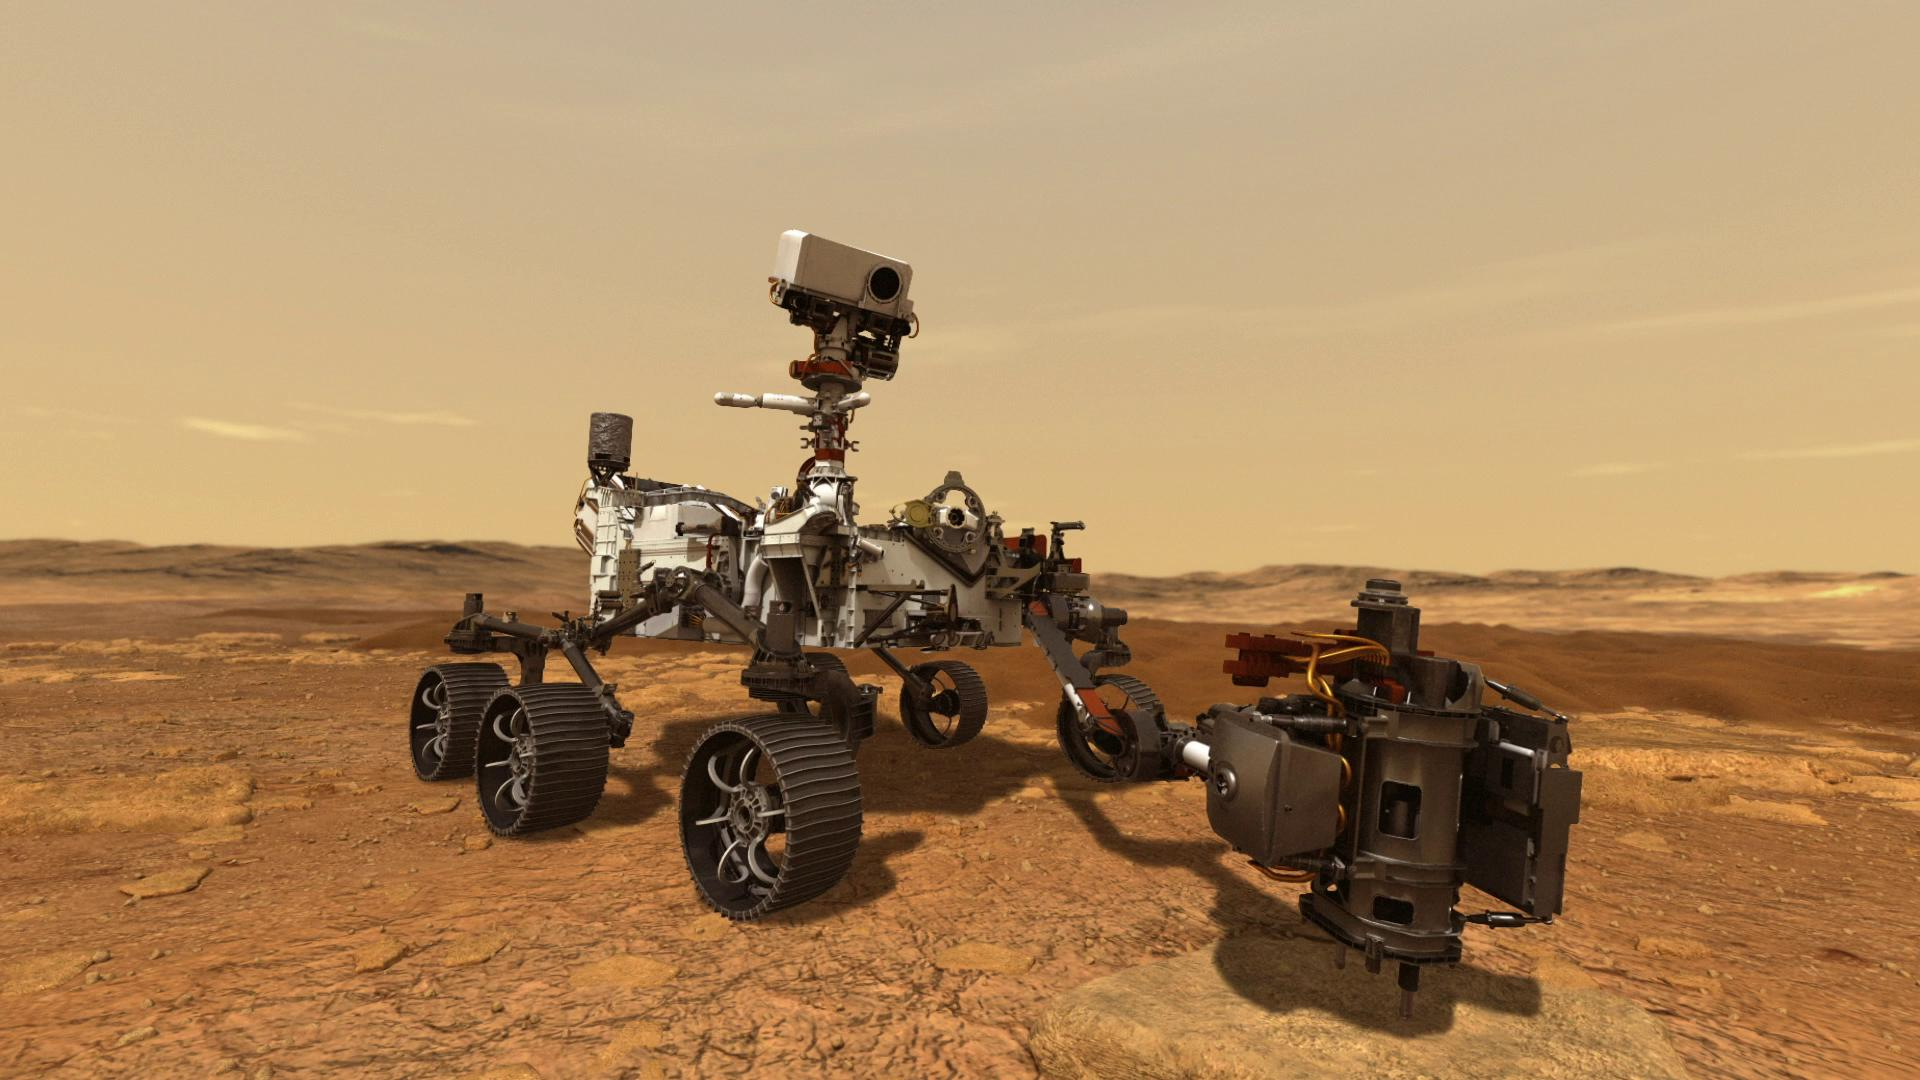
\includegraphics[width=.24\textwidth]{001a}\hfill
  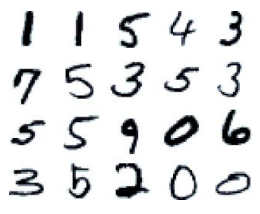
\includegraphics[width=.24\textwidth]{001b}\hfill
  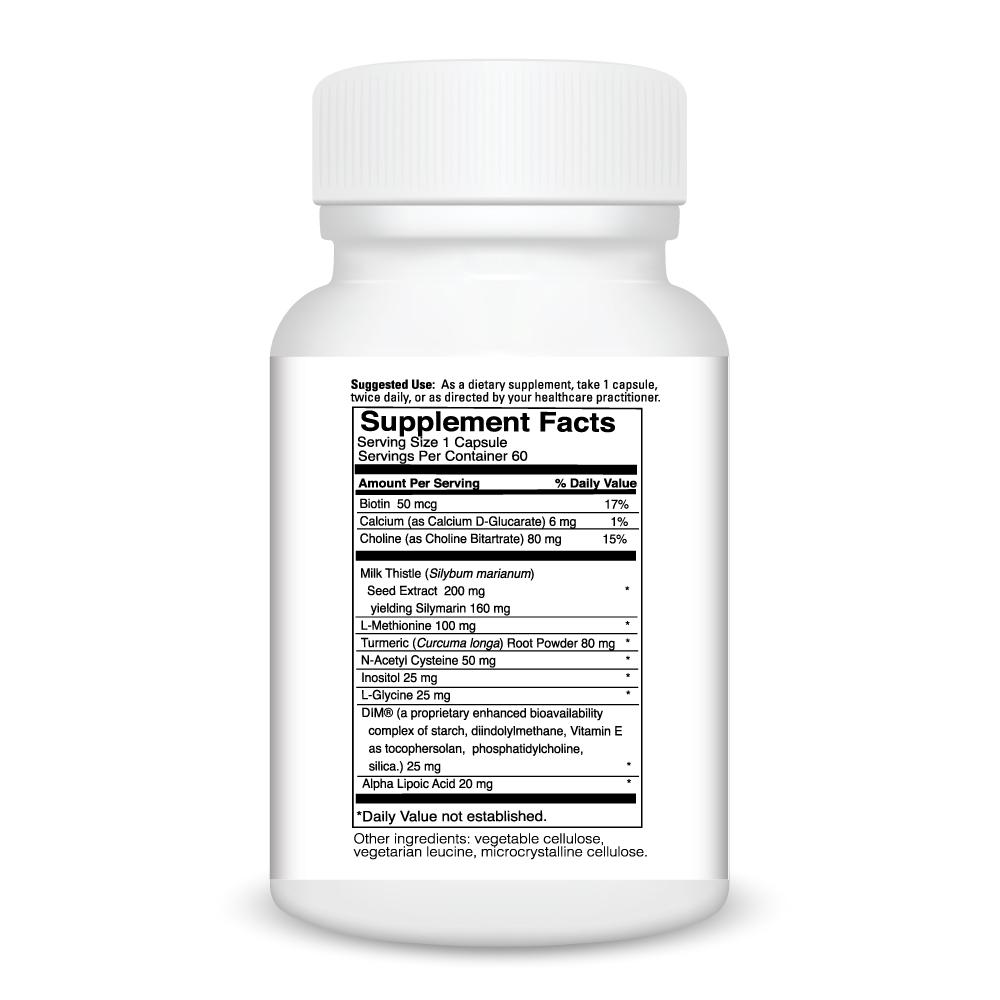
\includegraphics[width=.24\textwidth]{001c}\hfill
  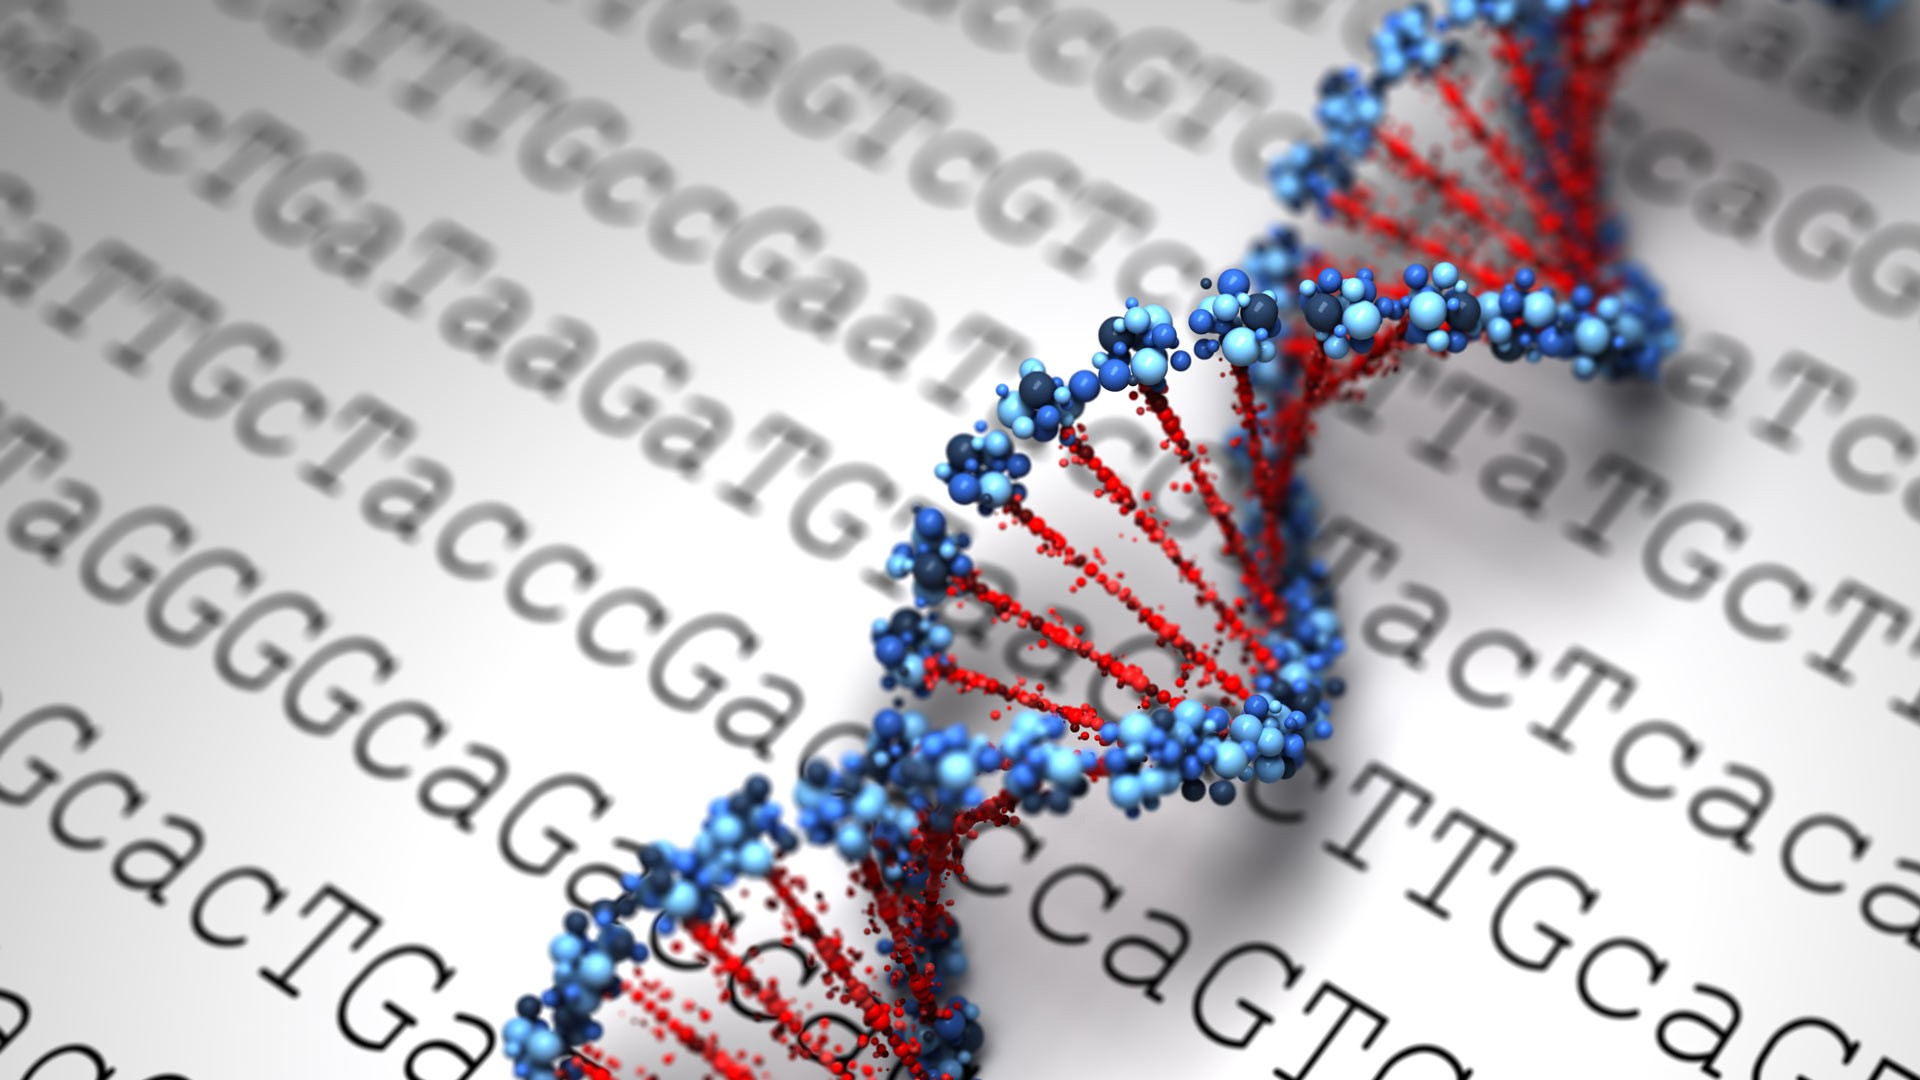
\includegraphics[width=.24\textwidth]{001d}
\end{figure*}

ML can be used for \textbf{recognizing} patterns, for example handwritten digits, facial and medical images; it can be used for \textbf{generating} patterns, for example for generating images or motion sequences; it can be used for recognizing anomalies, for example unusual credit card transactions or unusual patterns of sensor readings; or it can be used for \textbf{predictions}, for example it can be used to predict future stock prices or currency exchange rates, autonomous driving or to predict best moves in games.

\section{Definition}
Machine learning studies computer algorithms for learning to do stuff. We might, for instance, be interested in learning to complete a task, or to make accurate predictions, or to behave intelligently. The learning that is being done is always based on some sort of observations or data, such as examples, direct experience, or instruction. So in general, machine learning is about learning to do better in the future based on what was experienced in the past. Some more technical definitions have been provided during the development of machine learning:
\begin{itemize}[itemsep=.2em]
    \item It is concerned with the automatic discovery of regularities in data through the use of computer algorithms and with the use of these regularities to take actions. --- Chrisopher M. Bishop
    \item The goal of machine learning is to deveop methods that can automatically detect patterns in data, and then to use the uncovered patterns to predict future data or other outcomes of interest. --- Kevin P. Murphy
    \item Machine learning is about predicting the future based on the past. --- Hal Daume III
    \item A computer program is said to learn form \textbf{experience} \(E\) with resepct to some class of \textbf{tasks} \(T\) and performance \textbf{measure} \(P\), if its performance at tasks in \(T\), as measured by \(P\), improves with experience \(E\). --- T. Mitchell
\end{itemize}

\begin{figure}[t!]
  \begin{center}
  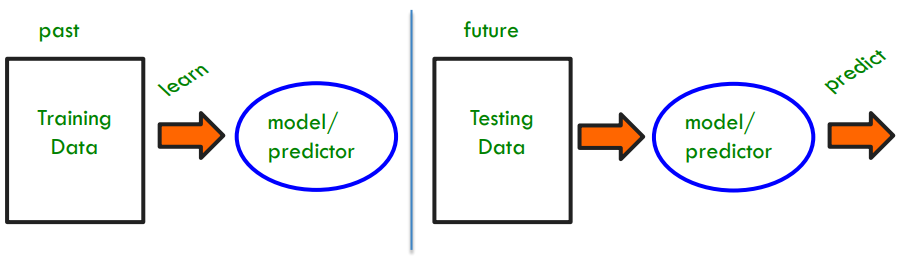
\includegraphics[width=0.75\textwidth]{002}
  \end{center}
\end{figure}

\subsection{Formally}
Mathematically speaking, machine learning is the study of algorithms that improve their performance \(P\) at some task \(T\) with experience \(E\). A well-defined learning task is given by a triplet \( \langle T,P,E \rangle \).

\begin{example}[Tasks for machine learning applications]
    For handwritten word recognition, the learning task \( \langle T,P,E \rangle \) is defined as follows:
    \begin{itemize}
        \item[T:] Recognizing handwritten words;
        \item[P:] Percentage of words correctly classified;
        \item[E:] Database of human-labeled images of handwritten words.
    \end{itemize}
    \tcblower
    For the spam email recognition, the learning task \( \langle T,P,E \rangle \) is defined as follows:
    \begin{itemize}
      \item[T:] Categorizing email messages as spam or legitimate;
      \item[P:] Percentage of email messages correctly classified;
      \item[E:] Database of emails, some with human-given labels.
    \end{itemize}
\end{example}

\section{Machine Learning vs Other Disciplines}
Modern day machine learning has two objectives, one is to classify data based on models which have been developed, the other purpose is to make predictions for future outcomes based on these models. A hypothetical algorithm specific to classifying data may use computer vision of moles coupled with supervised learning in order to train it to classify the cancerous moles. Where as, a machine learning algorithm for stock trading may inform the trader of future potential predictions.

\subsection{Artificial Intelligence}
\begin{wrapfigure}{r!}{0.35\textwidth}
    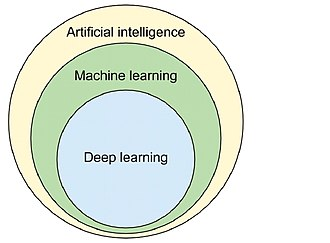
\includegraphics[width=0.35\textwidth]{003}
    \caption{Machine Learning as subfield of AI}
  \label{fig:003}
\end{wrapfigure}
Artificial intelligence (AI) is intelligence demonstrated by machines, as opposed to natural intelligence displayed by animals including humans. Leading AI textbooks define the field as the study of "intelligent agents": any system that perceives its environment and takes actions that maximize its chance of achieving its goals.

Some popular accounts use the term "artificial intelligence" to describe machines that mimic "cognitive" functions that humans associate with the human mind, such as "learning" and "problem solving", however, this definition is rejected by major AI researchers.

AI applications include advanced web search engines (e.g., Google), recommendation systems (used by YouTube, Amazon and Netflix), understanding human speech (such as Siri and Alexa), self-driving cars (e.g., Tesla), automated decision-making and competing at the highest level in strategic game systems (such as chess and Go). As machines become increasingly capable, tasks considered to require "intelligence" are often removed from the definition of AI, a phenomenon known as the AI effect. For instance, optical character recognition is frequently excluded from things considered to be AI, having become a routine technology.

\subsection{Deep Learning}
\begin{wrapfigure}{l!}{0.35\textwidth}
  \begin{center}
    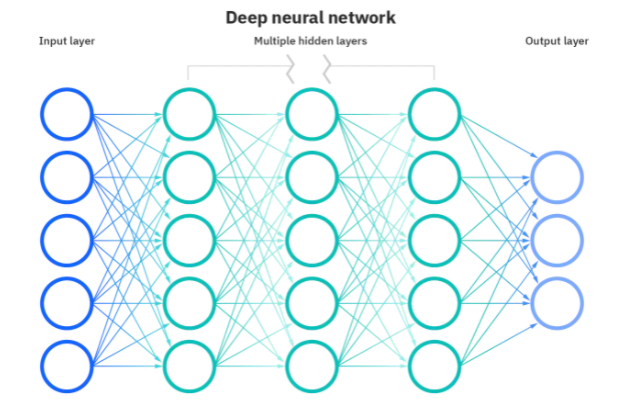
\includegraphics[width=0.35\textwidth]{004}
  \end{center}
  \label{fig:004}
\end{wrapfigure}
Deep Learning is part of a broader family of machine learning methods based on artificial neural networks with representation learning. Artificial neural networks (ANNs) were inspired by information processing and distributed communication nodes in biological systems. ANNs have various differences from biological brains. Specifically, artificial neural networks tend to be static and symbolic, while the biological brain of most living organisms is dynamic (plastic) and analogue.

The adjective "deep" in deep learning refers to the use of multiple layers in the network. Early work shows that a linear perceptron\footnote{\textbf{Perceptron:} is an algorithm for supervised learning of binary classifiers --- a function which can decide whether or not an input belongs to some specific class.} cannot be a universal classifier, but that a network with a nonpolynomial activation function with one hidden layer of unbounded width can. Deep learning is a modern variation which is concerned with an unbounded number of layers of bounded size, which permits pratical application and optimized implementation, while retaining theoretical universality under mild conditions. In deep learning the layers are also permitted to be heterogeneous and to deviate widely from biologically informed connectionist models, for the sake of efficiency, trainability and understandability, whence the "structured" part.

In deep learning, each level learns to transform its input data into a slightly more abstract and composite representation. In an image recognition application, the raw input may be a matrix of pixels; the first representational layer may abstract the pixels and encode edges; the second layer may compose and encode arrangements of edges; the third layer may encode a nose and eyes; and the fourth layer may recognize that the image contains a face. Importantly, a deep learning process can learn which features to optimally place in which level on its own. This does not eliminate the need for hand-tuning; for example, varying numbers of layers and layer sizes can provide different degrees of abstraction.

\subsection{Data Mining}
Data mining is a process of searching, extracting and analyzing (that may include) discovering various types of text graphic patterns (as calligraphic for example), language and literary figures, stylistics, in large amounts of textual or mixed visual and textual data sets, that also involvs methods at the intersection of machine learning, formal linguistics analyses as textual statistics, and database systems.

The actual data mining task is the semi-automatic or automatic analysis of large quantities of textual databases to extract previously not well known or entirely unknown, interesting or surprising language or information patterns such as groups of textual data records, but also unusual records (sometimes computer detected as anomaly), but also associations or dependencies (rule of pattern association and sequential pattern mining). This usually involves using database techniques such as using of spatial indices. These textual or information patterns can then be seen as summarizing of the input data, and may be used in further analysis or, for example, in machine learning for analysis involving predictions.

\section{Back to machine learning}

The general set up of predicting the future based on the past is at the core of most machine learning. The objects that our algorithm will make predictions about are \textbf{examples}. Let's consider for example the Netflix recommender system: when you watch a movie and state that you liked (or disliked) it, Netflix takes this as an example, and the like or dislike as a label that will make the algorithm learn from this example. 

\begin{wrapfigure}{r!}{0.35\textwidth}
  \begin{center}
    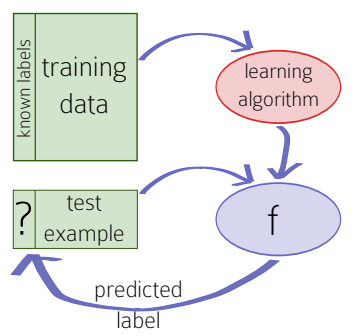
\includegraphics[width=0.35\textwidth]{005}
  \end{center}
  \caption{}
  \label{fig:005}
\end{wrapfigure}

To make this concrete, Figure~\ref{fig:005} shows the general framework of induction. We are given \textbf{training data} on which our algorithm is expected to learn. This training data is the examples that Alice observes, or the historical rating data for the recommender system. 
Based on this training data, our learning algorithm induces a function \(f\) that will map a new example to a corresponding prediction.

We want our algorithm to be able to make lots of predictions, so we refer to the collection of examples on which we will evaluate our algorithm as the \textbf{test set}. The test set is a closely guarded secret: it is the final exam on which our learning algorithm is being testes. 

The goal of inductive machine learning is to take some training data and use it to induce a function \(f\). This function \(f\) will be evaluated on the test data. The machine learning algorithm has succeeded if its performance on the test data is high.

\newpage
\begin{exercise}[topsep=20pt,itemsep=10pt]
  \ex When is Machine Learning recommended and when it is not? Give some example.
  \ex Give some example of Machine Learning algorithms on real applications.
  \ex Give the formal definition of Machine Learning and provide some example of task.
  \ex Provide the definition of Artificial Intelligence and Deep Learning enphasizing the differences from Machine Learning.
  \ex What are the examples?
  \ex How are the training data and the test data used?
\end{exercise}
% \chapter{Data, Features, and Models}
\begin{chapquote}{Kevin P. Murphy}
    ``The goal of machine learning is to develop methods that can automatically detect patterns in data, and then to use the uncovered patterns to predict future data or other outcomes of interest.''
\end{chapquote}

At a basic level, machine learning is about predicting the future based on the past. For instance, you might wish to predict how much a user Alice will like a movie that she hasn't seen, based on her ratings of movies that she has seen. This prediction could be based on many factors of the movies; in general, this means making informed guesses about some unobserved property of some object, based on observed properties of that object.

\section{The learning process}

\begin{figure}[h]
\begin{center}
    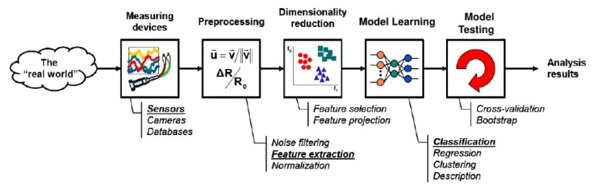
\includegraphics[width=.95\textwidth]{015}
\end{center}
\caption{Learning process scheme}
\label{fig:015}
\end{figure}

From the data we acquire knowledge, which is represented by a model, the model is used on future data.

In Figure~\ref{fig:015} we have a simplified pipeline of the learning process, divided by stages. 

The \textbf{measurement} can come from different sensors or database, these data are obtained in different ways, and then they are preprocessed. 

The \textbf{preprocessing} depends on the application, for example it can be noise filtering for measurements done when working with sensonrs. We need to transform our data in a set of vectore, called \emph{feature}, this operation is called \emph{feature extraction}. It is common, in many application, to do a normalization, which can be achieved in different ways.

Usually, feature extracted from the data are not directly fed into the model, but there is a selection (or projection) of the vectors to \textbf{reduce their dimensionality} and maintaining only useful information. Then, the machine learning algorithm is applied, it can differ depending on the different task of the applcation. Once we have outputted our model from the chosen algorithm, the testing phase is performed.

\section{Data}

\textbf{Data} are individual facts, statistics, or items of information, often numeric. In a more technical sense, data are a set of values of qualitative or quantitative variables about one or more persons or objects, while a \emph{datum} is a single value of a single variable.

\begin{wrapfigure}{r}{0.35\textwidth}
      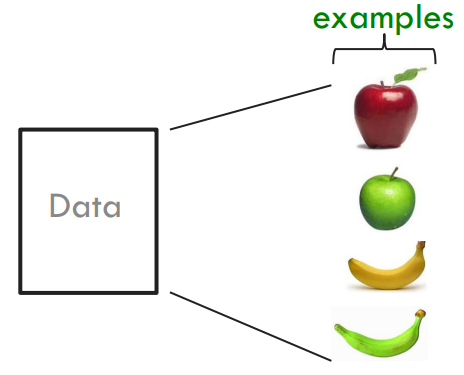
\includegraphics[width=0.35\textwidth]{006}
\end{wrapfigure}
Data are measured, collected, reported, and analyzed, and used to create data visualizations such as graphs, tables or images. Data as a general concept refers to the fact that some existing information or knowledge is represented or coded in some form suitable for better usage or processing.

We want to have a single way to treat our information and the same approach to represent the data. For each example in my training set, we have to translate these examples in terms of feature. Feature is usually a set of numbers, one example will be represented by a vector of cardinality \(N\).

\emph{Raw data} is a collection of numbers or characters before it has been \emph{cleaned} and corrected by researchers. Data processing commonly occurs by stages, and the processed data from one stage may be considered the raw data of the next stage.

Data is the most important part of all Data Analytics, Machine Learning, Artificial Intelligence. Without data, we can't train any model and all modern research and automation will go in vain.

\textbf{Information} is data that has been interpreted and manipulated and has now some meaningful inference for the user.

\textbf{Knowledge} is the combination of inferred information, experiences, learning, and insights. Results in awareness or concept building for an individual organization. Data can be split into:
\begin{itemize}
    \item \textbf{Training data}: the part of data we use to train our model. This is the data that the model actually sees (both input and output) and learns from.
    \item \textbf{Validation data}: the part of data that is used to do a frequent evaulation of the mode, fit on the training dataset along with improving involved hyperparameters (initially set parameters before the model begins learning). This data plays its part when the model is actually training.
    \item \textbf{Testing data}: once our model is completely trained, testing data provides an unbiased evaluation. When we feed in the inputs of testing data, our model will predict some values. After prediction, we evaluate our model by comparing it with the actual output present in the testing data. This is how we evaluate and see how much our model has learned from the experiences feed in as training data, set at the time of training. 
\end{itemize}

\subsection{Data Split}
Data is the information about the problem to solve in the form of a distribution, for classification and regression: \(p_{\text{data}} \in \Delta (X \times Y)\), for density estimation, clustering and dimensionality reduction: \(p_{\text{data}} \in \Delta (X)\). The data distribution \(p_{\text{data}}\) is typically unknown, but we can sample from it.

In machine learning, a common task is the study and construction of algorithms that can learn from and make predictions on data. Such algorithms function by making data-driven predictions or decisions, through building a mathematical model from input data. These input data used to build the model are usually divided in multiple data sets.

\subsubsection{Training set}
The model is initially fit on a \textbf{training data set}, which is a set of example used to fit the parameters of the model. The model is trained on the training set using a supervised learning method. In practice, the training set often consists of pairs of an input vector and the corresponding output vector, where the answer key is commonly denoted as the \emph{target}. The current model is run with the training set and produces a result, which is then compared with the target, for each input vector in the training set. Based on the result of the comparison and the specific learning algorithm being used, the parameters of the model are adjusted. The model fitting can include both variable selection and parameter estimation.

A training set is a set of examples used during the learning process and is used to fit the parameters of, for example, a classifier.

For classification tasks, a supervised learning algorithm looks at the training set to determina, or learn, the optimal combinations of variables that will generate a good predictive model. The goal is to produce a trained (fitted) model that generalizes well to new, unknown data. The fitted model is evaluated using new examples from the held-out datasets to estimate the model's accuracy in classifying new data. To reduce the risk of issues such as over-fitting, the examples in the validation and test datasets should not be used to train the model.

\begin{example}[Training set example]
\begin{wrapfigure}{l}{0.25\textwidth}
\begin{center}
    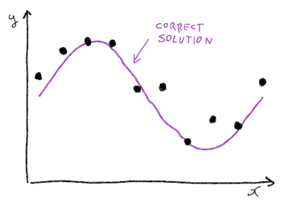
\includegraphics[width=0.25\textwidth]{017}
    \label{fig:017}
\end{center}
\end{wrapfigure}
Given the data \(D_n=\{(x_1,y_1),...,(x_n,y_n)\}\) generated from \(\sin(2 \pi x) + \)noise.\\
\\
The training set is made of pair, and is represented by \(n=10\) black dots. In the left figure we can see a graphical representtion of the training set. This data could serve for a task of regression.

\end{example}

\subsubsection{Validation test}
A \textbf{validation set} is a date set of examples used to tune the hyperparameters\footnote{\textbf{Hyperparameter:}  parameter whose value is used to control the learning proces. An example for artificial neural networks includes the number of hidden units in each layer.} of a classifier. It should follow the same probability distribution as the training set.

In order to avoid overfitting, when any classification parameter needs to be adjusted, it is necessary to have a validation set in addition to the training and test set. For example, if the most suitable classifier for the problem is sought, the training data set is used to train the different candidate classifiers, the validation data set is used to compare their performances and decide which one to take and, finally, the test set is used to obtain the performance characteristics such as accuracy, sensitivity, specificity, and so on. The validation set functions as a hybrid: it is training data used for testing, but neither as part of the low-level training nor as part of the final testing.

\subsubsection{Test set}
The \textbf{test data set} is a data set used to provide an unbiased evaluation of a final model fit on the training set. If the data in the test set has never been used in training, the test set is also called \textbf{holdout set}.

A test set is a data set that is independent of the training set, but that follows the same probability distribution. If a model fit to the training set also fits the test set well, minimal overfitting has taken place. A better fitting of the training data set as opposed to the test set usually points to over-fitting.

A test set is therefore a set of examples used only to assess the performance of a fully specified classifier. To do this, the final model is used to predict classifications of examples in the test set. Those predictions are compared to the examples' true classifications to assess the model's accuracy.

\begin{figure}[h]
\begin{center}
    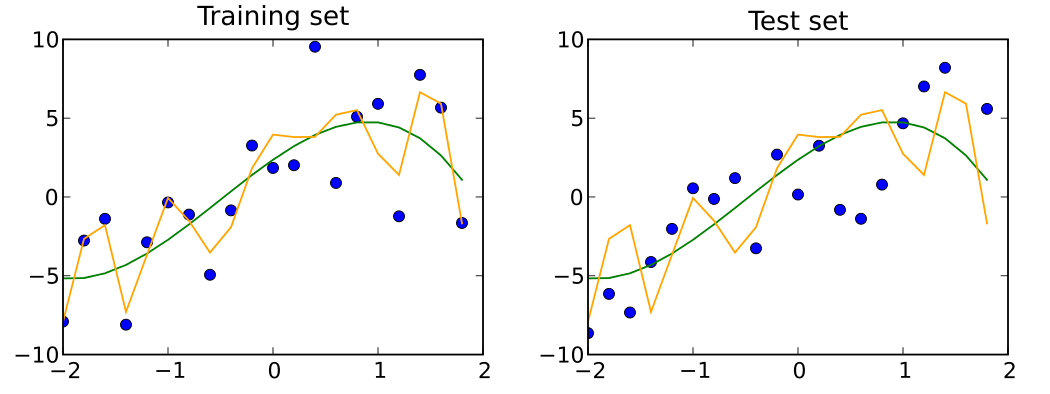
\includegraphics[width=.75\textwidth]{013}
    \caption{}
\end{center}
\caption{A training set and a test set from the same statistical population are shown as points. Two predictive models are fit to the training data. Both fitted models are plotted with both the training and test sets.}
\end{figure}

\subsection{Data generating distribution}
Our assumption is that learning problems are characterized by some unknown probablity distribution \(D\) over an input/output pairs \((x,y) \in X \times Y\). 

The training and test data are generated by a probability distribution overdatasets called the \textbf{data-generating process}. We typically make a set of assumptions known collectively as the i.i.d. assumptions. These assumptions are that the examples in each dataset are independent from each other, and thatthe training set and test set are identically distributed, drawn from the same probability distribution as each other. 

This assumption enables us to describe the data-generating process with a probability distribution over a single example. The same distribution is then used to generate every train example and every testexample. We call that shared underlying distribution the \textbf{data-generating distribution}, denoted \(p_data\). This probabilistic framework and the i.i.d. assumptions enables us to mathematically study the relationship between training error and test error.
\begin{figure}[h]
\begin{center}
    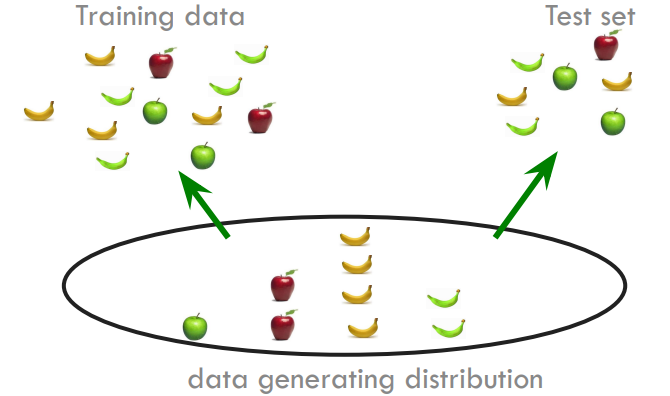
\includegraphics[width=.5\textwidth]{014}
    \caption{}
\end{center}
\caption{Example of a data generating distribution.}
\end{figure}


\section{Feature}
In machine learning and pattern recognition, a \textbf{feature} is an individual measurable property or characteristic of a phenomenon. Choosing informative, discriminating and independent features is a crucial element of effective algorithms in pattern recognition, classification and regression. Feature are usually numeric, but structural feature such as strings and graphs are used in syntactic pattern recognition. The concept of feature is related to that of explanatory variable used in statistical techniques such as linear regression.

\begin{wrapfigure}{l}{0.25\textwidth}
    \begin{center}
      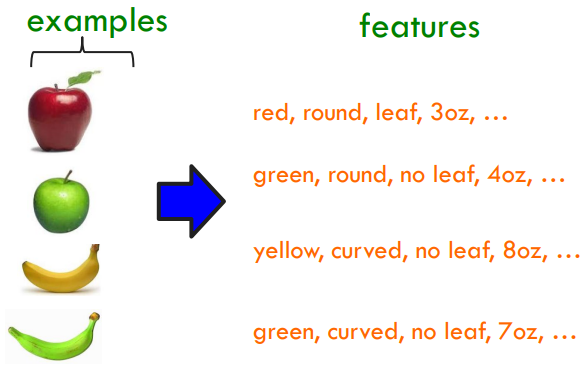
\includegraphics[width=0.25\textwidth]{007}
    \end{center}
\end{wrapfigure}

One of the most important aspect of machine learning model is identifying the features which will help create a great model, the model that performs well on unseen data. The initial set of raw features can be redundant and too large to be managed. Therefore, a preliminary step in many applications of machine learning and pattern recognition consists of selecting a subset of features, or constructing a new and reduced set of features to facilitate learning, and to improve generalization and interpretability. Extracting or selecting features is a combination of art and science; developing systems to do so is known as feature engineering. It requires the experimentation of multiple possibilities and the combination of automated techniques with the intuition and knowledge of the domain expert. Automating this process is feature learning, where a machine not only uses features for learning, but learns the features itself.

A \textbf{feature vector} is an \(n\)-dimensional vector of numerical features that represent some object. Many algorithms in machine learning require a numerical representation of objects, since such representations facilitate processing and statistical analysis. Feature vectors are often combined with weights using a dot product in order to construct a linear predictor function that is used to determine a score for making a prediction.

The vector spaces associated with these vector is often called \textbf{feature space}. In order to reduce the dimensionality of the feature space, a number of dimensionality reduction techniques can be employed.

Higher-level features can be obtained from already available features and added to the feature vector. This process is referred to as feature construction. Feature construction is the application of a set of constructive operators to a set of existing features resulting in construction of new features. Feature construction has long been considered a powerful tool for increasing both accuracy and understanding of structure, particularly in high-dimensional problems.

\subsection{Characteristics of good features}
A great feature must satisfy the following criteria, that are the characteristics of good features:
\begin{itemize}[topsep={0pt}, partopsep={0pt}]
    \item Features must be found in most of the data samples: Great features represent unique characteritistics which can be applied across different types of data samples and are not limited to just one data sample. For example, can the “red” color of apple act as a feature? Not really. Because apple can be found in different colors. It might have happened that the sample of apples that was taken for evaluation contained apple of just “red” color. If not found, we may end up creating models having high bias. 
    \item Features must be unique and may not be found prevalent with other (different) forms: Great features are the ones which is unique to apple and should not be applicable for other fruits. The toughness characteristic of apple such as “hard to teeth” may not be good feature. This is because a guava can also be explained using this feature. 
    \item Features in reality: There can be features which can be accidental in nature and is not a feature at all when considering the population. For example, in a particular sample of data, a particular kind of feature can be found to be prevalent. However, when multiple data samples are taken, the feature goes missing. 
\end{itemize}

\begin{figure}[t!]
    \begin{center}
        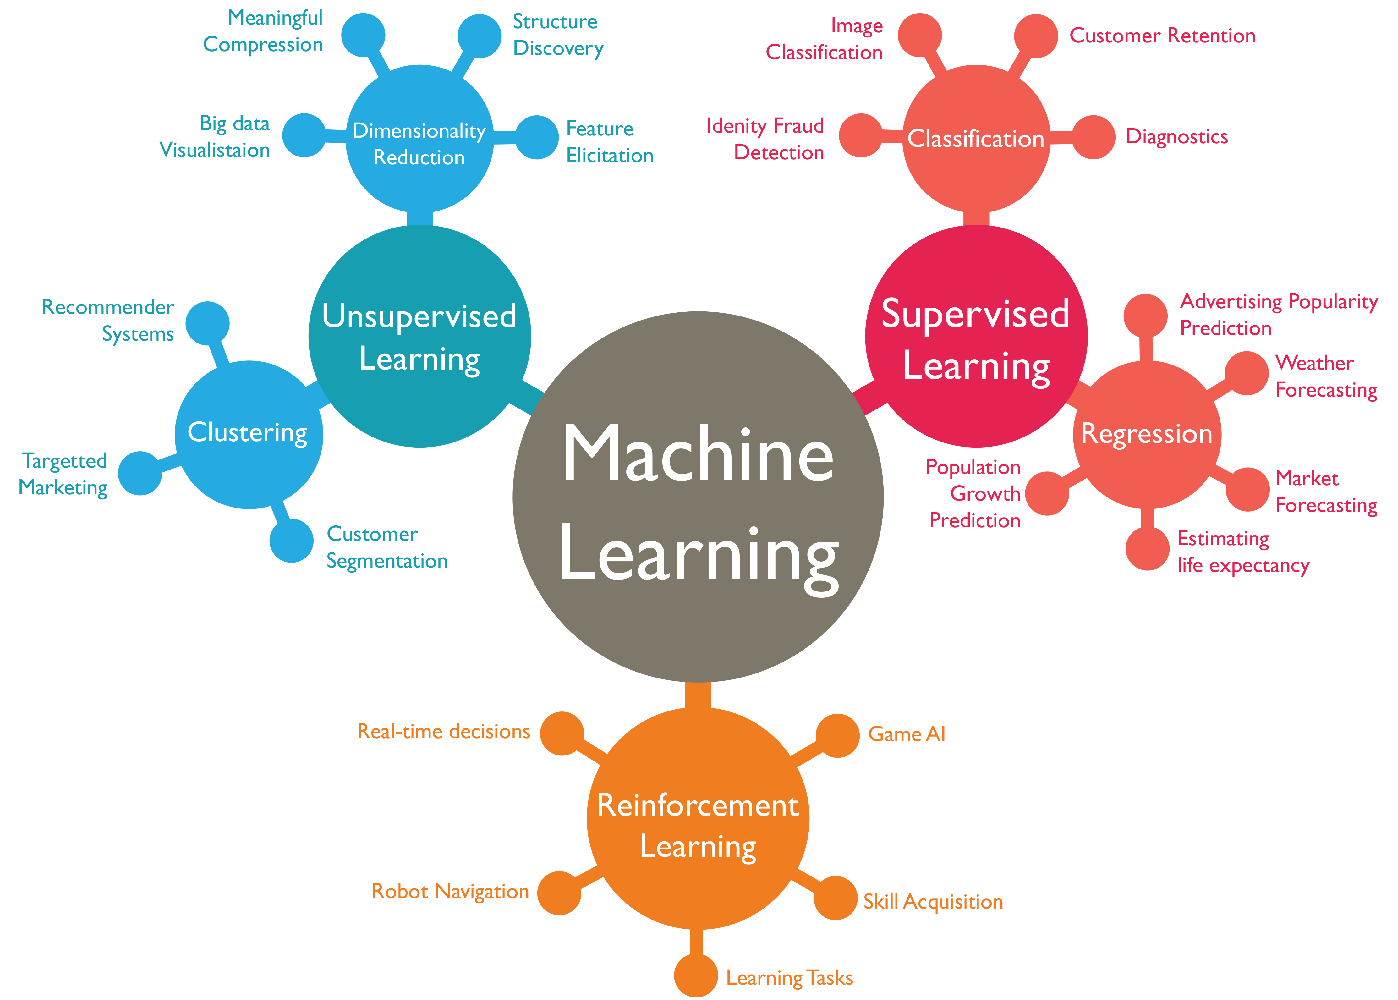
\includegraphics[width=\textwidth]{037}
    \end{center}
    \caption{Types of learning map}
    \label{fig:037}
\end{figure}

\section{Types of learning}
Machine learning approeaches are traditionally divided into three broad categories, depending on the nature of the \emph{signal} or \emph{feedback} available to the learning system. Machine Learning has found its applications in almost every business sector. There are several algorithms used in machine learning that help you build complex models. Each of these algorithms in machine learning can be classified into a certain category.

There are primarily three types of machine learning:
\begin{itemize}[topsep={0pt}, partopsep={0pt}]
    \item Supervised Learning;
    \item Unsupervisde Learning;
    \item Reinforcement Learning.
\end{itemize}

\subsection{Supervised learning}
\begin{wrapfigure}{l}{0.25\textwidth}
      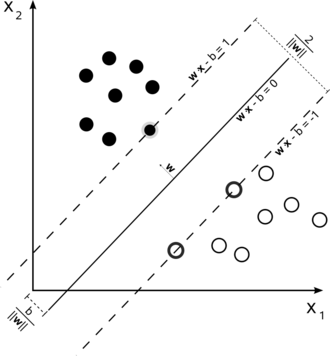
\includegraphics[width=0.25\textwidth]{008}
\end{wrapfigure}
Supervised learning algorithms build a mathematical model of a set of data that contains both the inputs and the desired outputs. The training data consists of a set of training examples. Each training example has one or more inputs and the desired output, also known as a supervisory signal. 

Through iterative optimization of an objective function, supervised learning algorithms learn a function that can be used to predict the ouput associated with new inputs. An optimal function will allow the algorithm to correctly determine the output for inputs that were not a part of the training data. An algorithm that improves the accuracy of its outputs or predictions over time is said to have learned to perform that task.

Supervised learning uses a training set to teach models to yield the desired output. This training dataset includes inputs and correct outputs, which allow the model to learn over time. The algorithm measures its accuracy through the loss function\footnote{We will talk more about loss functions in the next chapters.}, adjusting until the error has been sufficiently minimized.

We can resume the supervised learning in the following definition: Supervised learning is the machine learning task of learning a function that maps an input to an output based on example input-output pairs. It infers a function from labeled training data consisting of a set of training examples. In supervised learning, each example is a pair consisting of an input object (typically a vector) and a desired output value.

\subsubsection{Classification}
Classification is the problem of identifying which of a set of categories an observation belongs to. An algorithm that implements classification, especially in a concrete implementation, is known as a \emph{classifier}. The term also refers to the mathematical function, implemented by a classification algorithm, that maps input data to category.

Classification is a process of categorizing a given set of data into classes, It can be performed on both structured or unstructured data. The process starts with predicting the class of given data points. The classes are often referred to as target, label or categories.

The classification predictive modeling is the task of approximating the mapping function from input variables to discrete output variables. The main goal is to identify which class/category the new data will fall into.

We can divide the classification problem into two subproblems, that are binary classification and multiclass classification:
\begin{itemize}
\item \textbf{Binary classification: } It is a type of classification with two outcomes, for eg – either true or false. Given a training set \(T = \{(x_1,y_1), ..., (x_m, y_m)\}\). Learn a function \(f\) to predict \(y\) given \(x\). \(y\) is categorical, \(d=1\).
\[f: \mathbb{R}^d \to \{1,2,...,k\}\]
\item \textbf{Multiclass classification: } The classification with more than two classes, in multi-class classification each sample is assigned to one and only one label or target.. Given a training set \(T = \{(x_1,y_1), ..., (x_m, y_m)\}\). Learn a function \(f\) to predict \(y\) given \(x\). \(x\) is multidimensional (multiple features).
\[f: \mathbb{R}^d \to \{1,2,...,k\}\]
\end{itemize}

\begin{figure}[h!]
    \centering
    \begin{subfigure}{.4\textwidth}
        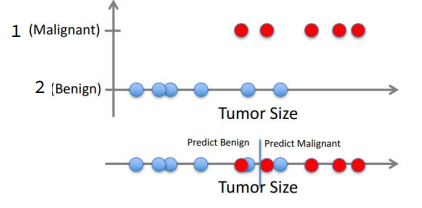
\includegraphics[width=1\textwidth]{009}
        \caption{Binary}
    \end{subfigure}
    \begin{subfigure}{.4\textwidth}
        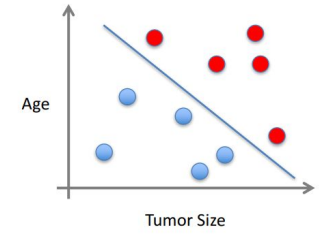
\includegraphics[width=1\textwidth]{010}
        \caption{Multiclass}
    \end{subfigure}
    \caption{Classification example}
\end{figure}

\begin{figure}[b]
    \centering
    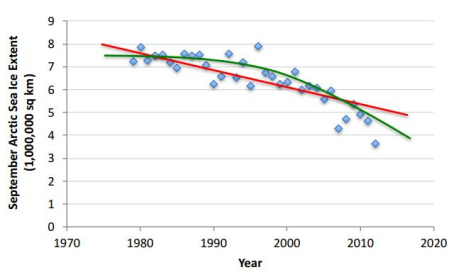
\includegraphics[width=.6\textwidth]{011}
    \caption{Regression}
\end{figure}

\subsubsection{Regression}
Regression analysis is a set of statistical processes for estimating the relationships between a dependent variable and one or more independent variables. The most common form of regression analysis is linear regression, in which one finds the line that most closely fits the data according to a specific mathematical criterion.

The following article provides an outline for Regression in Machine Learning. Regression means to predict the value using the input data. Regression models are used to predict a continuous value. It is mostly used to find the relationship between the variables and forecasting. Regression models differ based on the kind of relationship between dependent and independent variables.

Given a training set \(T = \{(x_1,y_1), ..., (x_m, y_m)\}\). Learn a function \(f\) to predict \(y\) given \(x\). \(y\) is real-valued \(d=1\).
\begin{equation}
    f: \mathbb{R}^d \to \mathbb{R}
\end{equation} 

Linear regression is employed in varied ways in which a number of them are listed as:
\begin{itemize}[topsep={0pt}, partopsep={0pt}]
\item Sales prognostication
\item Risk analysis
\item Housing applications
\item Finance applications
\end{itemize}

\subsubsection{Ranking}
Ranking is the data transformation in which numerical or ordinal values are replaced by their rank when the data are sorted.  Training data consists of lists of items with some partial order specified between items in each list. This order is typically induced by giving a numerical or ordinal score or a binary judgment (e.g. "relevant" or "not relevant") for each item. The goal of constructing the ranking model is to rank new, unseen lists in a similar way to rankings in the training data.

For example, the ordinal data \emph{hot}, \emph{cold}, and \emph{warm} would be replaced by \(3\), \(1\), \(2\).

\begin{example}
    Training data consists of queries and documents matching them together with relevance degree of each match. It may be prepared manually by human assessors (or raters, as Google calls them), who check results for some queries and determine relevance of each result. It is not feasible to check the relevance of all documents, and so typically a technique called pooling is used — only the top few documents, retrieved by some existing ranking models are checked. This technique may introduce selection bias. Alternatively, training data may be derived automatically by analyzing clickthrough logs (i.e. search results which got clicks from users), query chains, or such search engines' features as Google's (since-replaced) SearchWiki. Clickthrough logs can be biased by the tendency of users to click on the top search results on the assumption that they are already well-ranked.
\end{example}

\subsection{Unsupervised learning}
Unsupervised learning algorithms take a set of data that contains only inputs, and find structure in the data, like grouping or clustering of data points. The algorithms, therefore, learn from test data that has not been labeled, classified or categorized. 

Unsupervised learning uses machine learning algorithms to analyze and cluster unlabeled datasets. These algorithms discover hidden patterns or data groupings without the need for human intervention. Its ability to discover similarities and differences in information make it the ideal solution for exploratory data analysis, cross-selling strategies, customer segmentation, and image recognition.

Instead of responding to feedback, unsupervised learning algorithms identify commonalities in the data and react based on the presence or absence of such commonalities in each new piece of data.

\begin{figure}
    \begin{center}
        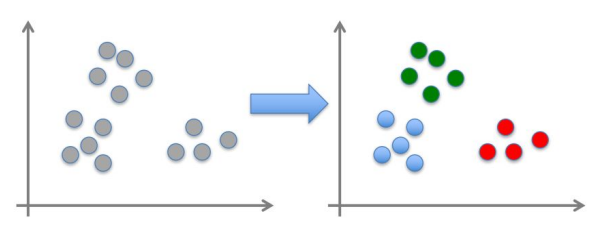
\includegraphics[width=.6\textwidth]{012}
    \end{center}
    \caption{Clustering}
    \end{figure}
    
\subsubsection{Clustering}
Cluster analysis is the assignment of a set of observations into subsets (called \emph{clusters}) so that observations within the same cluster are similar according to one or more predesignated criteria, while observations drawn from different clusters are dissimilar. 

Cluster analysis itself is not one specific algorithm, but the general task to be solved. It can be achieved by various algorithms that differ significantly in their understanding of what constitutes a cluster and how to efficiently find them. Popular notions of clusters include groups with small distances between cluster members, dense areas of the data space, intervals or particular statistical distributions. Clustering can therefore be formulated as a multi-objective optimization problem. The appropriate clustering algorithm and parameter settings (including parameters such as the distance function to use, a density threshold or the number of expected clusters) depend on the individual data set and intended use of the results. Cluster analysis as such is not an automatic task, but an iterative process of knowledge discovery or interactive multi-objective optimization that involves trial and failure. It is often necessary to modify data preprocessing and model parameters until the result achieves the desired properties.

Formally, given \(T = \{x_1, ..., x_m\}\) without labels, the output is the hidden structure behind the \(x\)'s, that is the cluster.

\subsubsection{Anomaly detection}
Anomaly detection is the identification of rare items, events or observations which raise suspicions by differing significantly from the majority of the data.
In data analysis, anomaly detection (also referred to as outlier detection) is generally understood to be the identification of rare items, events or observations which deviate significantly from the majority of the data. Such examples may arouse suspicions of being generated by a different mechanism, or appear inconsistent with the data.

Typically the anomalous items will translate to some kind of problem such as bank fraud, a structural defect, medical problems or errors in a text. Anomalies are also referred to as outliers, novelties, noise, deviations and exceptions.

Anomaly detection is applicable in a very large number and variety of domains, and is an important subarea of unsupervised machine learning. As such it has applications in cyber-security intrusion detection, fraud detection, fault detection, system health monitoring, event detection in sensor networks, detecting ecosystem disturbances, defect detection in images using machine vision, medical diagnosis and law enforcement.

\subsubsection{Dimensionality reduction}
Dimensionality reduction is a process of reducing the number of random variables under consideration by obtaining a set of principal variables. It is a process of reducing the dimension of the feature set, also called \emph{number of features}. Most of the dimensionality reduction techniques can be considered as either feature elimination or extraction.

Dimensionality reduction, or dimension reduction, is the transformation of data from a high-dimensional space into a low-dimensional space so that the low-dimensional representation retains some meaningful properties of the original data, ideally close to its intrinsic dimension. Working in high-dimensional spaces can be undesirable for many reasons; raw data are often sparse as a consequence of the curse of dimensionality, and analyzing the data is usually computationally intractable (hard to control or deal with). Dimensionality reduction is common in fields that deal with large numbers of observations and/or large numbers of variables, such as signal processing, speech recognition, neuroinformatics, and bioinformatics.

Dimensionality reduction can be used for noise reduction, data visualization, cluster analysis, or as an intermediate step to facilitate other analyses.

\subsection{Reinforcement learning}
Reinforcement learning is an area of machine learning concerned with how intelligent agents ought to take actions in an environment in order to maximize the notion of cumulative reward. 

Reinforcement learning is the training of machine learning models to make a sequence of decisions. The agent learns to achieve a goal in an uncertain, potentially complex environment. In reinforcement learning, an artificial intelligence faces a game-like situation. The computer employs trial and error to come up with a solution to the problem. To get the machine to do what the programmer wants, the artificial intelligence gets either rewards or penalties for the actions it performs. Its goal is to maximize the total reward.
Although the designer sets the reward policy-that is, the rules of the game-he gives the model no hints or suggestions for how to solve the game. It's up to the model to figure out how to perform the task to maximize the reward, starting from totally random trials and finishing with sophisticated tactics and superhuman skills. By leveraging the power of search and many trials, reinforcement learning is currently the most effective way to hint machine's creativity. In contrast to human beings, artificial intelligence can gather experience from thousands of parallel gameplays if a reinforcement learning algorithm is run on a sufficiently powerful computer infrastructure.
\begin{figure}[t!]
    \begin{center}
        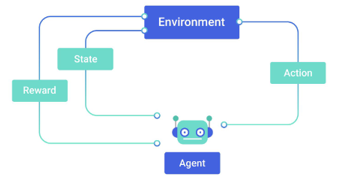
\includegraphics[width=.6\textwidth]{016}
    \end{center}
    \caption{Reinforcement learning flow chart}
    \label{fig:016}
\end{figure}

Training the models that control autonomous cars is an excellent example of a potential application of reinforcement learning. In an ideal situation, the computer should get no instructions on driving the car. The programmer would avoid hard-wiring anything connected with the task and allow the machine to learn from its own errors. In a perfect situation, the only hard-wired element would be the reward function.

\subsection{Other Learning Types}
- semi-supervised learning,
- active learning,
- online vs offline learning,
- generative vs discriminative,
- parametric vs non-parametric.

\newpage
\begin{exercise}[topsep=20pt,itemsep=10pt]
    \ex Describe the learning process and each of its step.
    \ex What is data? How can be split? How is it used in Machine Learning?
    \ex Provide the definitions of Information and Knowledge.
    \ex What is a feature? What is a feature vector? What do they represent? 
    \ex Provide the definitions of the three types of learning.
    \ex Provide the definitions of classification, regression, and ranking.
    \ex[!] What is multiclass classification?
    \ex Provide the definitions of clustering, anomaly detection, and dimensionality reduction.
    \ex[!] What is dimensionality reduction? What is it useful for? What are its benefits?
    \ex What is Reinforcement Learning? Provide a basic flow chart.
    \ex[!] What is the difference between supervised learning and reinforcement learning?
\end{exercise}
% \chapter{Generalization error, Models, Hypothesis space}
\begin{chapquote}{A. Samuel}
    ``Machine learning is the science of getting computers to act without being explicitly programmed.''
\end{chapquote}

Machine learning is a very general and useful framework, but won't always work. In order to better understand when it will and when it will not work, it is useful to formalize the learning problem more.

\section{Task}
Tasks represent the type of prediction being made to solve a problem on some data. We can identify a task with the set of functions that can potentially solve it. In general, it consists of functions assigning each input \(x \in X\) an output \(y \in Y\).
\[f: X \to Y \qquad F_{\text{task}} \subset Y^X\]
The nature of \(X\), \(Y\) and \(F_{\text{task}}\) depends on the type of task.

\paragraph{Classification task}
The task for classification is to find a function \(f \in Y^X\) assigning each input \(x \in X\) a discrete label.
\[f(x) \in Y = \{c_1,...,c_k\}\]
Common classification applicaton are face recognition, character recognition, spam detection, medical diagnosis (from symptoms to illnesses), and biometrics.

\paragraph{Regression task}
The task for regression is to find a function \(f(x) \in Y\) assigning each input a \emph{countinuous} label.
Example of applications for regression task are in the field of economics/finance (predict the value of a stock), epidemiology, car/plane navigation (angle of the steering wheel, acceleration, ...), temporal trends (weather over time)..

\paragraph{Density estimation}
Density estimation is the construction of an estimate, based on observed data, of an unobservable underlying probability density function. The unobservable density function is thought of as the density according to which a large population is distributed.

The task for density estimation is to find a probability distribution \(f \in \Delta (X) \)\footnote{\(\Delta (X)\) is the set of all the probability distributions.} that fits the data \(x \in X\). 

\paragraph{Clustering task}
The task for clustering is to find a function \(f \in \mathbb{N}^X\) that assigns each input \(x \in X\) a cluster index \(f(x) \in \mathbb{N}\). All points mapped to the same index form a cluster.

Some applications for clustering tasks are social network analysis and genomics (group individuals by genetic similarity).

\paragraph{Dimensionality reduction task}
The task for dimensionality reduction is to find a function \(f \in Y^X\) mapping each (high dimensional) input \(x \in X\) to a lower dimensional embedding \(f(x) \in Y\), where \(\text{dim}(Y) \ll \text{dim}(X)\), and \(Y=\mathbb{R}^2\).

\section{Model and hypotesis space}
A \textbf{model} in machine learning is the output of a machine learning algorithm run on data. A model represents what was learned by a machine learning algorithm.

The model is the thing that is saved after running a machine learning algorithm on training data and represents the rules, numbers, and any other algorithm-specific data structures required to make predictions.

\begin{example}
    \begin{itemize}
        \item
        The linear regression algorithm results in a model comprised of a vector of coefficients with specific values.
        \item
        The decision tree algorithm results in a model comprised of a tree of if-then statements with specific values.
        \item
        The neural network/backpropagation/gradient descent algorithm together results in a model comprised of a graph structure with vectors or matrices of weigths with specific values.
    \end{itemize}
\end{example}

A machine learning model is more challenging for a beginner because there is not a clear analogy with other algorithms in computer science. The best analogy is to think of the machine learning model as a program, comprised of both data and a procedure for using the data to make a prediction. It is the implementation of a function \(f \in F_{\text{task}}\) that can be computed. The function \(f\) is an abstract concept, and the  model is the implementation.

We assume that the set of all possible model is a subset \(H \subset F_{\text{task}}\), called \emph{hypotesis space}.

\begin{example}[Polynomial curve fitting]
    \begin{center}
        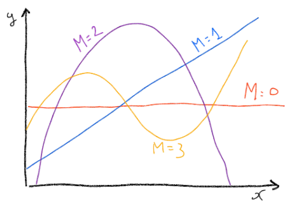
\includegraphics[width=0.4\textwidth]{018}
    \end{center}
    Data are the dots in the graph, and we want to learn the function. One way is to find the set of functions \(f\) and parametrize them with paremeter \(w\), multiplying with associated \(x\) to the power of \(j\). This corresponds to a polynomial of different degrees. 
    
    Model:
    \[f_w(x)= \sum_{j=0}^{M} w_jx^j\]
    Hypothesis space:
    \[H_M=\{f_w:w\in \mathbb{R}^M\}\]
    where \(H_M\) is the hypotesis space for fixed \(w \in \mathbb{N}\).
\end{example}

\subsection{The ideal target}
\begin{wrapfigure}{l}{0.35\textwidth}
\begin{center}
    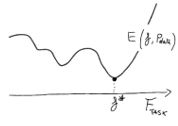
\includegraphics[width=0.35\textwidth]{019}
\end{center}
\label{fig:019}
\end{wrapfigure}
We want to minimize a generalization error function \(E(f;p_{\text{data}})\). The error function determines how well a solution \(f \in F_{\text{task}}\) fits some given data and guides the selection of the best solution in \(F_{\text{task}}\):
\[f^* \in arg\ \min_{f \in F_\text{task}} E(f; p_{\text{data}})\]

An error function tells how well my model fits some given data. Allows us to find the best \(f^*\) in the space of \(F_{\text{task}}\). Since this search space is too large and we do not have access to \(p_{\text{data}}\), we cannot complete this search, so we need an implementation for the error function.

\subsection{The feasible target}
\begin{wrapfigure}{l}{0.35\textwidth}
\begin{center}
    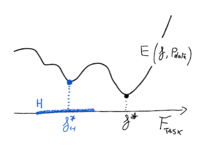
\includegraphics[width=0.35\textwidth]{020}
\end{center}
\label{fig:020}
\end{wrapfigure}
We need to restrict the focus on finding functions that can be implemented and evaluated in a tractable way. Thus we define a model and an hypotesis space \(H \subset F_{\text{task}}\) and seek a solution within that space.
\[f^*_H \in arg\ \min_{f\in H} E(f; p_{\text{data}})\]
We have restricted our search space, however we still may have some trouble computing the search, because \(p_{\text{data}}\) is unknown.

\subsection{The actual target}
\begin{wrapfigure}{l}{0.35\textwidth}
\begin{center}
    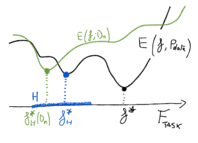
\includegraphics[width=0.35\textwidth]{021}
\end{center}
\label{fig:021}
\end{wrapfigure}
We need to revisit our minimization problem. Instead of using \(p_{\text{data}}\) we need to work on a data sample, i.e. a training set \(D_n=\{z_1,...,z_n\}\) where \(z_i=(x_i,y_i) \in X \times Y\), and \(z_i \sim p_{\text{data}}\).
\[f^*_H(D_n) \in arg\ \min_{f \in H} E(f; D_n)\]
This function is called training error and it does not match with the generalization error.

\section{Error function}
Machine learning can be thought of as an optimization problem, where there is an objective function that needs to be either maximized or minimized, and the best solution is the model that achieves either the highest or lowest score respectively. 

Typically in machine learning problems, we seek to minimize the error between the predicted value vs the actual value. The word \emph{error} represents the penalty of failing to achieve the expected output. If the loss is calculated for a single training example, it is called or \textbf{error function}. If the same loss is averaged across the entire training sample, the loss is called cost function.

Error function vary with the type of problem we are trying to solve. Regression problems that attempt to predict a continuous value have one set of loss functions, while the classification problems where the algorithm attempts to classify the training example into one of the target classes have another set of error/cost function.

Typically, the generalization and training error function can be written in terms of a pointwise loss \(l(f; z)\) measuring the error incurred by \(f\) on the training example \(z\).

\begin{align}
    &E(f; p_{\text{data}}) = E_{z \sim p_{\text{data}}}[l(f;z)]\\
    &E(f;D_n) = \frac 1 n \sum^n_{i=1}l(f;z_i)
\end{align}

\begin{figure}[h]

\label{fig:022}
\end{figure}
\begin{example}[Polynomial curve fitting]
\begin{center}
    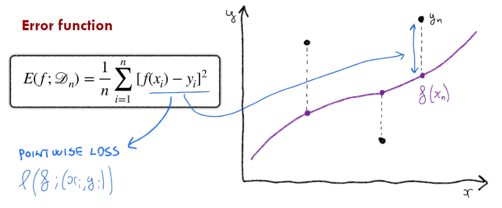
\includegraphics[width=0.6\textwidth]{022}
\end{center}
The pointwise loss is computed on each sample \(x_i\) separately. In this case it makes sense to have the square term, in this way we have the so called \emph{square loss}. Given our training data, we compute \(y_i\) and our function \(f\). Our objective is:
\[f^*_{H_M}(D_n) \in arg\ \min_{f \in H_M} E(f;D_n)\]
The objective is equivalent to \(f_{w^*}\), where \(w^*\) is defined as follows:
\[w^* \in arg\ \min_{w \in \mathbb{R}^M} \frac 1 n \sum^n_{i=1} [f_w(x_i)-y_i]^2\]
This requires to solve a linear system of equations.

\end{example}

Our learning algorithm solves the optimization problem targeting \(f_H^*(D_n)\), but might end up in a different result.
\begin{figure}[h]
\begin{center}
    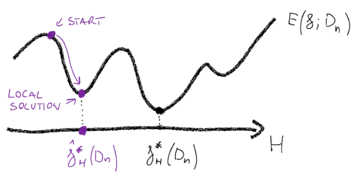
\includegraphics[width=0.5\textwidth]{023}
    \caption{}
    \label{fig:023}
\end{center}
\end{figure}

Let us put all the charts together, and build a recap chart for the \(f^*(D_n)\) function, showing the training error and the generalization error.
% TODO: add to summary
% \begin{figure}[h]
% \begin{center}
%     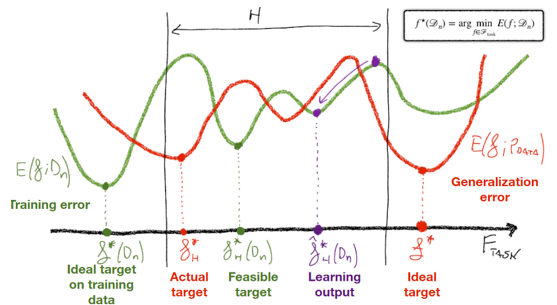
\includegraphics[width=0.75\textwidth]{024}
%     \caption{}
%     \label{fig:024}
% \end{center}
% \end{figure}

After performing our search, we obtain our learning output, this could introduce two potential problems, overfitting and underfitting.
\begin{figure}[h]
\begin{center}
    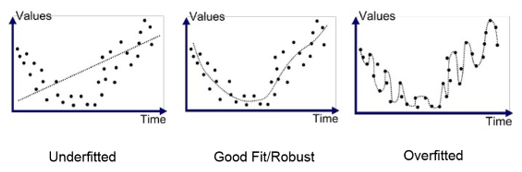
\includegraphics[width=0.75\textwidth]{025}
    \caption{Graphical representation of curve fitting}
\end{center}
\end{figure}

\subsection{Overfitting}
\textbf{Overfitting} is the production of an analysis that corresponds too closely or exactly to a particular set of data, and may therefore fail to fit additional data or predict future observations reliably.

An overfitted model is a statistical model that contains more parameters than can be justified by the data. The essence of overfitting is to have unknowningly extracted some of the residual variatione (i.e., the noise) as if the variation represented underlying model structure.

Overfitting occurs when the learned function \(\Hat{f}_H^*\), becomes sensitive to the noise in the sample. As the result, the function will perform well on the training set but not perform well on other data from the joint probability distribution of \(x\) and \(y\). Thus, the more overfitting occurs, the larger the generalization error.

\subsection{Underfitting}
\textbf{Underfitting} occurs when a machine learning algorithm cannot adequately capture the underlying structure of the data. It occurs when the model or algorithm shows low variance but high bias. It is often a result of an excessively simple model which is not able to process the complexity of the problem. This results in a model which is not suitable to handle all the signal and is therefore orced to take some signal as noise. 

If instead a model is capable to handle the signal but anyways takes a part of it as noise as well, it is also considered to be underfitted. The latter case can happen if the loss function of a model includes a penalty which is too high in that specific case.

An underfitted model would ignore some important replicable structure in the data and thus fail to identify effects that were actually supported by the data. In this case, bias in the parameter estimators is often substantial, and the sampling variance is underestimated, both factors resulting in poor confidence interval coverage. Underfitted models tend to miss important treatment effects in experimental settings.

\subsection{Estimate the generalization error}
The generalization error cannot be computed for \(p_{\text{data}}\), because it's unknown. The only possible way to access generalization error is by sampling. We use a data sample, and we assume that the probability distribution is the same for the training set, for the validation set, and for the test set.

We use the training set to find the best model, then the validation set to find the best hyperparameters. Once we have done this operation, we may think of having a way to estimate the generalization error in order to understand if the model will work well on the test data.

\begin{example}[Polynomial curve fitting]
\begin{center}
    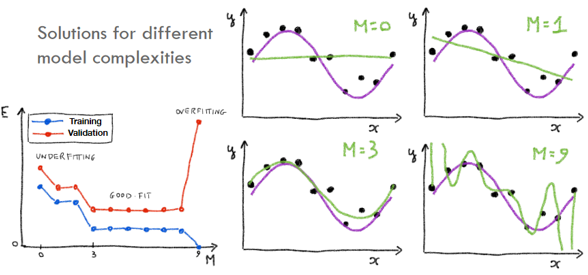
\includegraphics[width=0.75\textwidth]{026}
    \label{fig:026}
\end{center}
With the first model in Figure~\ref{fig:026}, there is an underfitting, high error, low performance in training and validation set. On the other side, with the last model there is overfitting, we approximate with almost 0 errors on training data, while performing poorly on unknown test data represented by smooth curve.

\end{example}

\subsection{Improve the generalization}
In order to improve generalization well, one needs to avoid both underfitting of the training data and overfitting of the training data.

There are a number of approeaches for improving generalization, one can:
\begin{itemize}
    \item
    Avoid to obtain the minimum on training error;
    \item
    Reduce the model capacity;
    \item
    Change the objective with a regularization term;
    \item
    Inject noise in the learning algorithm to smooth out the data points;
    \item
    Stop the learning algorithm before the convergence to avoid the model to learn too well on training data.
\end{itemize}

\subsubsection{Regularization}
The regularization is the modification of the training error function with a term \(\Omega(f)\) that typically penalizes complex solutions.
\[E_{\text{reg}}(f;D_n) = E(f;D_n) + \lambda_n \Omega (f)\]
We are adding another function \(\Omega\) to force the algorithm to learn a model with low complexity. It penalizes complex solution to find a simpler one, which can find a model that generalizes better (so to find a better \(f^*\)). The \(\lambda_n\) is a trade-off parameter.

\begin{example}[Polynomial curve fitting]
We regularize by penalizing polynomials with large coefficients:
\[E_{\text{reg}}(f;D_n) = \frac 1 n \sum_{i=1}^n [f_w(x_i)-y_i]^2 + \frac \lambda n ||w||^2\]
\[||w||^2 = \sum_i=w_i^2\]
We invoke norm regularization and set lambda hyperparameters by considering performance on validation set. The lambda parameter regulates the trade-off between underfitting and overfitting

% \begin{figure}[t!]
%     \begin{center}
%         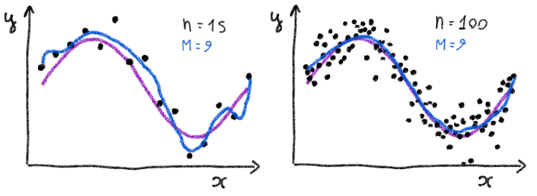
\includegraphics[width=0.75\textwidth]{028}
%         \caption{Generalization vs. data size for the polynomial curve fitting.}
%         \label{fig:028}
%     \end{center}
% \end{figure}

% \begin{figure}[h]
% \begin{center}
%     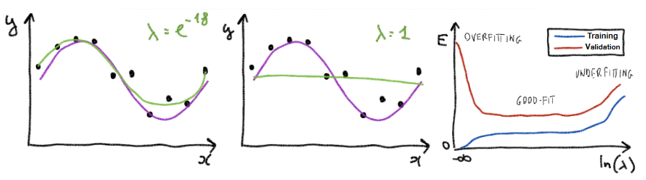
\includegraphics[width=0.75\textwidth]{027}
%     \caption{}
%     \label{fig:027}
% \end{center}
% \end{figure}

\end{example}

There are other approaches one can attempt, for example:
\begin{itemize}
    \item
    Increase the amount of data;
    \item
    Add more training samples;
    \item
    Augment the training set with transformations, when the provious is not possible;
    \item
    Combine prediction from multiple, decorrelated models to have preditions that are independent, and merging them we will probably get better labels. This technique is called \emph{ensembling}.
\end{itemize}

\begin{example}[Polynomial curve fitting]
Let's see the modification of the generalization in respect to the data size.
\[E(f;D_n) \to E(f;p_{\text{data}}) \qquad \text{as } n \to \infty\]
A graphical representation is provided in Figure~\ref{fig:028}.

\begin{center}
    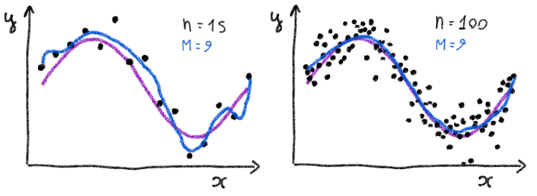
\includegraphics[width=0.75\textwidth]{028}
    \label{fig:028}
\end{center}
\end{example}

\newpage
\begin{exercise}[topsep=20pt, itemsep=10pt]
\end{exercise}

% \part{Supervised Learning}
% \chapter{\(k\)-Nearest Neighbor}
After having introduced all the basics of machine learning, we start talking about the specific algorithm in order to address at the beginning of supervised classification problem. The first algorithm we present is one of the simplest one, and it is the \textbf{K-Nearest Neighbor}.

\section{Introduction}

K-Nearest Neighbor classifier is one of the introductory supervised classifiers, which every data science learner should be aware of. This algorithm was first used for a pattern classification task which was first used by Fix \& Hodges in 1951. To be similar the name was given as KNN classifier. KNN aims for pattern recognition tasks.  

K-Nearest Neighbor also known as KNN is a supervised learning algorithm that can be used for regression as well as classification problems. Generally, it is used for classification problems in machine learning. 

In \textbf{KNN classification}, the output is a class membership. An object is classified by a plurality vote of its neighbors, with the object being assigned to the class most common among its \(k\) nearest neighbors (\(k\) is a positive integer, typically small). If \(k=1\), then the object is simply assigned to the class of that single nearest neighbor. 

In \textbf{KNN regression} the output is the property value for the object. This value is the average of the values of \(k\) nearest neighbors.

Both for classification and regression, a useful technique can be to assign weights to the contributions of the neighbors, so that the nearer neighbors contribute more to the average than the more distant ones. For example, a common weighting scheme consists in giving each neighbor a weight of \(\frac 1 d\), where \(d\) is the distance to the neighbor.

\section{Algorithm}
\begin{wrapfigure}{l}{0.25\textwidth}
\begin{center}
    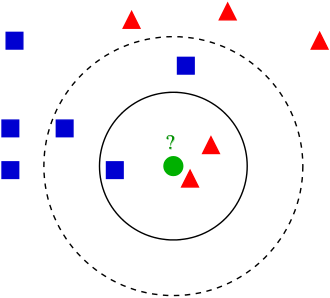
\includegraphics[width=0.25\textwidth]{029}
    \caption{}
    \label{fig:029}
\end{center}
\end{wrapfigure}
The training examples are vectors in a multidimensional feature space, each with a class label. The training phase of the algorithm consists only of storing the feature vectors and class labels of the training samples.

In the classification phase, \(k\) is a user-defined constant, and an unlabeled vector is classified by assigning the label which is most frequent amongh the \(k\) training samples nearest to that query point.

In Figure~\ref{fig:029} we have an example of KNN classification. The test sample (the green dot) should be classified either to blue squares or to red triangles. if \(k=3\) (solid line circle) it is assigned to the red triangles because there are two triangles and only one square. If \(k=5\) (dashed line circle) it is assigned to the blue squares.

To classify an example \(d\) you have to find the \(k\) nearest neighbors of \(d\), and then choose as the label the majority label within the \(k\) nearest neighbors. But how do we measure the \emph{nearest}?

\subsection{Euclidean distance}
The most common choice, is to compute the \textbf{euclidean distance} between the test sample and  his neighbors.

In two dimensions, given two points \(a(a_1, a_2)\) and \(b(b_1, b_2)\), the euclidean distance is computed as follows:
\[D(a,b) = \sqrt{(a_1-b_1)^2 + (a_2-b_2)^2}\]

In \(n\)-dimensions, we compute the distance in an analogous manner. Given two points \(a(a_1, a_2, ..., a_n)\) and \(b(b_1, b_2, ..., b_n)\), the euclidean distance is computed as follows:
\begin{align}
D(a,b)  &= \sqrt{(a_1-b_1)^2 + (a_2-b_2)^2 + ... + (a_n-b_n)^2}\\
        &=\sqrt{\sum_{d=1}^D(a_d-b_d)^2}
\end{align}

Measuring distance (or similarity) is a domain-specific problem and there are many, many differen variations.

\subsection{Algorithm}
\begin{algorithm}
\caption{kNN-classification($data$, $query$, $k$, $distance_{fn}$)}
\label{alg:knn}
$neighborDistance \gets [\ ]$\;
\ForEach{$(index, example) \in data$}{
    $distance \gets distance_{fn}(example.pop(), query)$\;
    $neigborDistance.append((distance,index))$\;
}
$sortedND \gets sort(neighborDistance)$\;
$kNNDistances \gets sortedND[k]$
\Comment*[r]{Get first k neighbors}
$kNNLabels \gets [kNNDistances.index]$
\Comment*[r]{Get labels of first k neighbors}
\Return{kNNDistances, Counter(labels).mostCommon()}
\end{algorithm}


\section{Decision boundaries}
The decision boundaries are areas in the features space where the classification of a point (example) changes.

Nearest neighbor rules implicitly compute the decision boundary. It is also possible to compute the decision boundary explicitly, and to do so efficiently, so that the computational complexity is a function of the boundary complexity.

Decision boundaries are useful ways to visualize the complexity of a learned model. Intuitively, a learned model with a decision boundary that is really jagged (like the coastline of Norway) is really complex and prone to overfitting. A learned model with a decision boundary that is really simple (like the bounary between Arizona and Utah) is potentially underfit.

In kNN, once you have chosen \(k\), kNN gives locally defined decision boundaries between classes, that depend on the choice of \(k\).

\section{Choosing \(k\)}

\begin{center}
    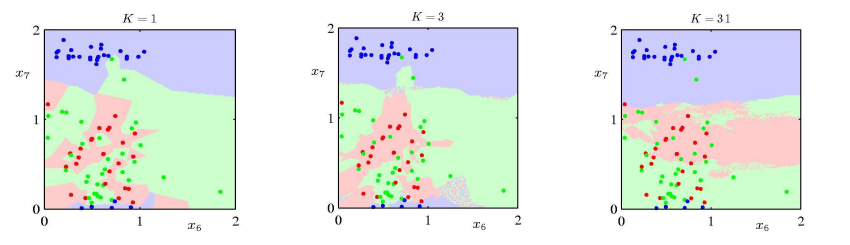
\includegraphics[width=0.75\textwidth]{030}
    \label{fig:030}
\end{center}

The best choice of \(k\) depends upon the data; generally, larger values of \(k\) reduces effect of the noise on the classification, but make boundaries between classes less distinct. A good \(k\) can be selected by various heuristic techniques. The special case where the class is predicted to be the class of the closest training sample (i.e. when \(k=1\) is called the nearest neighbor algorithm.

The accuracy of the kNN algorithm can be severely degraded by the presence of noisy or irrelevant features, or if the feature scales are not consistent with their importance. A particularly popular approach is the use of evolutionary algorithms to optimize feature scaling. Another popular approach is to scale fetures by the mutual information of the training data with the training classes. 

In binary classification problems, it is helpful to choose \(k\) to be an odd number as this avoids tied votes. One popular way of choosing the empirically optimal \(k\) in this setting is via bootstrap method.

\section{KNN in practice}
KNN's main disadvantage of becoming significantly slower as the volume of data increases makes it an impractical choice in environments where predictions need to be made rapidly. Moreover, there are faster algorithms that can produce more accurate classification and regression results.

However, provided you have sufficient computing resources to speedily handle the data you are using to make predictions, KNN can still be useful in solving problems that have solutions that depend on identifying similar objects. 

\subsection{Recommender Systems}
At scale, this would look like recommending products on Amazon, article on Medium, movies on Netflix, or videos on YouTube. Although, we can be certain they all use more efficient means of making recommendations due to the enormous volume of data they process.

\subsection{Weighted \(k\)-Nearest Neighbor}
The intuition behind weighted kNN, is to give more weight to the points which are nearby and less weight to the points which are farther away. Any function can be used as a kernel funcion for the weighted kNN classifier whose value decreases as the distance increases.

The \(k\)-nearest neighbor classifier can be viewed as assigning the \(k\) nearest neighbors a weight \(\frac 1 k\) and all others \(0\) weights. This can be generalised to weighted nearest neighbour classifiers. That is, where the \(i\)th nearest neighbour is assigned a weight \(w_{ni}\)m with \(\sum_{i=1}^nw_{ni}=1\). 

\subsubsection{Algorithm}
\begin{itemize}
    \item
    Let \(L=\{(x_i,y_i), i=1,2,...,n\}\) be a training set of observations \(x_i\) with iven class \(y_i\), and let \(x\) be a new observation (query point) whose class label \(y\) has to be predicted.
    \item
    Compute \(d(xi,x)\) for \(i=1,2,...,n\), the distance between the query point and every other point in the training set.
    \item
    Select \(D' \subset D\), the set of \(k\) nearest training data points to the query points.
    \item
    Predict the class of the query point, using distance-weighted voting. The \(v\) represents the class labels. Use the following formula:
    \begin{equation}
        y'=argmax_v \sum_{(x_i,y_i) \in D_z}w_i \times I(v=y_i)
    \end{equation}
\end{itemize}


% \chapter{Linear Models}

We now move over to discuss another simple model in Machine Learning, the class of \textbf{Linear Models}. Linear Models leads us to the introduction of \textbf{perceptrons}.

Some machine learning approaches make strong assumptions about the data: if the assumptions are true it can often lead to better performance, but if the assumptions are false the approach can fail miserably.
Other approaches don't make many assumptions about the data, this can allow us to learn from more varied data, but they are more prone to overfitting and generaly require more training data.

Linear models generate a formula to create a best-fit line to predict unknown values. Linear Models are considered not as predictive as newer algorithm classes, but they can be trained relatively quicky and are generally more straightforward to interpret, which can be a big plus.

\section{Bias}
The \textbf{bias} of a model is how strong the model assumptions are. Low-bias classifiers make minimal assumptions about the data (kNN and decision trees are generally considered low bias), high-bias classifiers make strong assumptions about the data.

A strong high-bias assumption is \textbf{linear separability}: in two dimenstions, can separate classes by a line, in higher dimensions, need hyperplanes.

A linear model is a model that assumes the data is linearly separable.

\subsection{Define a line}
Any pair of values \((w_1,w_2)\) defines a line through the origin: \(w_1f_1 + w_2f_2 = 0\).

\begin{example}
\begin{wrapfigure}{l}{0.25\textwidth}
\begin{center}
    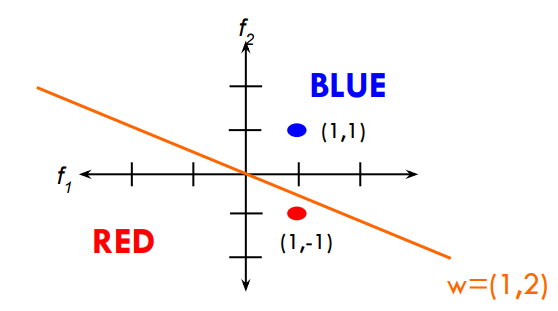
\includegraphics[width=0.25\textwidth]{031}
    \label{fig:031}
\end{center}
\caption{}
\end{wrapfigure}
For example, in Figure~\ref{fig:031} we have the line \(1f_1+2_2 = 0\). This equation means that we have our training data in a two-dimensional space, we have only two features (\(f_1\) and \(f_2\)), and the line that separate our training points is the orange line.

We can see the parameters \((w_1=1,w_2=2)\) as the vector perpendicular to the orange line. In fact, the orange line is perpendicular to the vector that starts from the origin \(O(0,0)\), and goes to the point \(w(1,2)\).

How can we classify mathematically the points based on a line? If we got two example data \(B(1,1)\) and \(R(1,-1)\), we have the following results:
\begin{align*}
(1,1) &: 1*1+2*1=3\\
(1,-1) &: 1*1+2*(-1)=-1
\end{align*}
The sign of the result indicates which side of the line is occupied by the example in the space.

\end{example}

We can move our line from the origin, if we use the following equation, that uses a parameter \(a\) in order to represent any line in a two dimensional space:
\[w_1f_1+w_2f_2=a\]
In this case we have a line intersects at \(a\) in the horizontal axis.

A linear model in \(n\)-dimensional space (i.e. \(n\) features) is defined by \(n+1\) weights. In two dimesions, we have a line 
\begin{equation}
    w_1f_1+w_2f_2+b=0 \qquad \text{where } b=-a
\end{equation}
In three dimensions, we have a plane
\[w_1f_1+w_2f_2+w_3f_3+b=0\]
In \(n\) dimensions, we have a \textbf{hyperplane}
\begin{equation}
    b+\sum_{i=1}^nw_if_i=0
\end{equation}

\subsection{Classifying with linear models}
Havin define the notion of line and the notion of hyperplane, we can show that a linear model, and in particular an hyperplane, can be used for classification by simply looking at the sign of the following equation:
\begin{equation}
\label{eqn:001}
b+\sum_{i=1}^nw_if_i
\end{equation}
if the result of equation \ref{eqn:001} is greater than \(0\), we have a positive example that belongs to the positive class; otherwise, if the result is lower than \(0\), we have a negative example that belongs to the negative class.

\section{Online learning}
\textbf{Online learning} is a method of machine learning in which data becomes available in a sequential order ad is used to update the best predictor for future data at each step, as opposed to batch learning techniques which generate the best predictor by learning on the etire training data set at once.

Online learning is able to overcome the drawbacks of batch learning in that the predictive model can be updated intantly for any new data instances. Thus, online learning algorithms are far more efficient and scalable for large-scale machine learning tasks in real-world data analytics applications where data are not only large in size, but also arriving at a high velocity.

\subsection{Tasks and applications}

Online learning algorithms can be derived for supervised learning tasks. One of the most common tasks is classification, aiming to predict the categories for a new data instance belongs to, on the basis of observing past training data instances whose category labels are given. For example, a commonly studied task in online learning is \textbf{online binary classification} (e.g., spam email filtering) which only involves two categories (“spam” vs “benign” emails); other types of supervised classification tasks include multi-class classification, multi-label classification, and multiple-instance classification, etc.

In addition to classification tasks, another common supervised learning task is \textbf{regression analysis}, which refers to the learning process for estimating the relationships among variables (typically between a dependent variable and one or more independent variables). Online learning techniques are naturally applied for regression analysis tasks, e.g., time series analysis in financial markets where data instances naturally arrive in a sequential way. Besides, another application for online learning with financial time series data is \textbf{online portfolio section} where an online learner aims to find a good (e.g., profitable and low-risk) strategy for making a sequence of decisions for portfolio selection.

\section{Perceptron}

The \textbf{perceptron} is an algorithm for supervised learning of binary classifiers. A binary classifier is a function which can decide wheter or not an input, represented by a vectior of numbers, belongs to some specific class. 

In the modern sense, the perceptron is an algorithm for learning a binary classifier called a \text{threshold function}: a function that maps its input \(x\) to an output value \(f(x)\):
\begin{equation}
    f(x) = \begin{cases}
        1               &\text{if \(w \cdot x + b > 0\), } \\
        0               &\text{otherwise}\\
    \end{cases}
\end{equation}
where \(w\) is a vector of real-valued weights, \(w \cdot x\) is the dot product \(\sum_{i=1}^mw_ix_i\), where \(m\) is the number of inputs to the perceptron, and \(b\) is the bias.

The value of \(f(x)\) is used to classify \(x\) as either a positive or a negative instance, in the case of a binary classification problem. If \(b\) is negative, then the weighted combination of inputs must produce a positive value greater thant \(|b|\) in order to push the classifier neuron over the 0 threshold.

Spatially, the bias alters the position of the decision boundary. The perceptron learning algorithm does not terminate if the learning set is not linearly separable. If the vectors are not linearly separable learning will never reach a point where all vectors are classified properly. 

\subsection{Convergence and number of iterations}
We will have convergence when the data are linearly separable, but when data is not linearly separable, we have to set up a number of iterations, otherwise the algorithm will fall in an infinite loop.

The training instances are linearly separable if, given two classes of examples, there exists a hyperplane that will separate the two classes.

The number of iterations can be used to prevent the overfitting of the perceptron algorithm.

\subsection{Algorithm}

\begin{algorithm}
\caption{Perceptron learning}
\label{alg:perceptron}
\While{convergence not reached}{
    \ForEach{training example $f_i$, $label$}{
        $prediction \gets b + \sum_{i=1}^nw_if_i$
        \Comment*[r]{check if it is correct}
        \If{not correct}{
            \ForEach{$w_i$}{
                $w_i \gets w_i + f_i \cdot label$
                \Comment*[r]{update all the weights}
            }
            $b \gets b + label$\;
        }
    }
}
\end{algorithm}

\begin{center}
    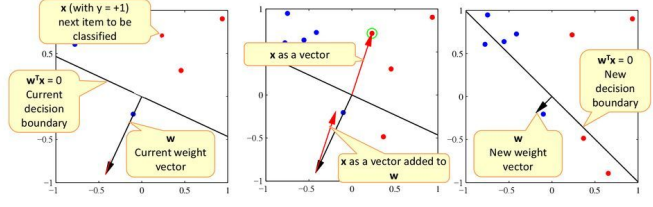
\includegraphics[width=0.75\textwidth]{032}
    \label{fig:032}
\end{center}

The perceptron algorithm guarantees that finds \textbf{some} line that separates the data, but we have no guarantees that the perceptron have found a special line. This will be especially important when we will discuss the difference between the perceptron and the Support Vector Machine.
% \chapter{Decision trees}

Decision tree learning is one of the predictive modeling approaches used in machine learning. It uses a decisione tree as a predictive model to go from observations about an item (represented in the branches) to conclusions about the item's target value (represented in the leaves). Tree models where the target variable can take a discrete set of values are called \textbf{classification trees}; in these tree structures, leaves represent class labels and branches represent conjunctions of features that lead to those class labels. Decision trees where the target variable can take continuous values are called \textbf{regression trees}. Decision trees are among the most popular machine learning algorithms given their intelligibility and simplicity.

\begin{wrapfigure}{r}{0.25\textwidth}
    \begin{center}
        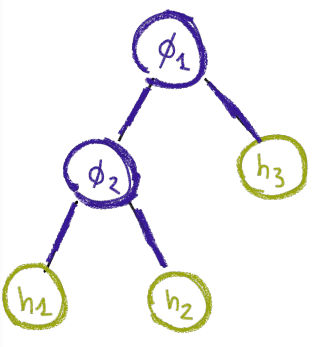
\includegraphics[width=0.25\textwidth]{033}
        \label{fig:033}
    \end{center}
    \caption{}
    \vspace{-40pt}
\end{wrapfigure}

A decision tree is a non-parametric supervised learning algorithm, it has a hierarchical tree structure, which consists of a root node, branches, internal nodes, and leaf nodes. The concept of a decision tree is to select splits that decrease the impurity of class distribution in the resulting subsets of instances. At the same time, the domination of one or more classes over the other classes is increased. This way, you can find a subset that contains only instances of one class after a few splits. For decision trees, binary trees are referred because they can be generalized better than trees with high-cardinality attributes.

\section{How decision trees work}
A decision tree starts with a root node, which does not have any incoming branches. The outgoing branches from the root node then feed into the internal nodes, also knows as \textbf{decision nodes}. Based on the available features, both node types conduct evaluations to form homogeneous subsets, which are denoted by leaf nodes, or terminal nodes. The leaf nodes represent all the possible outcomes within the dataset.

A decision tree takes an input \(x \in X\), the growing starts from a single root node, and routes it through its nodes until it reaches a leaf node. Each non-terminal node \(Node(\phi, t_L, t_r)\) holds a routing function \(\phi \in \{L,R\}^X\), a left child \(t_L\) and a right child \(t_R\). When \(x\) reaches the node it will go to the left child \(t_L\) or the right child \(t_R\) depending on the value of \(\phi(x) \in \{L,R\}\). When you do a split, each of the created descendant nodes corresponds to the applicable subset of the training data set. Further splits of these nodes result in new nodes that correspond to smaller subsets of data sets, and so on. Nodes that are not split further become leaves, each leaf node \(Leaf(h)\) holds a prediction function \(h \in F_\text{task}\) (typically a constant), depending on the task we want to solve it can be \(h \in Y^X\) (classification or regression) or \(h \in \Delta(X)\) (density estimation) or other. Once \(x\) reaches the leaf, the final prediction is given by \(h(x)\).

Decision tree learning employs a divide and conquer strategy by conducting a greed search to identify the optimal split points within a tree. this process of splitting is then repeated in a top-down, recursive manner until all, or the majority of records have been classified under specific class labels.

\subsubsection{Inference}
In order to infer with the decision tree, we define \(f_t\), the function returning the prediction for input \(x \in X\) according to the decision tree \(t\), that is recursively defined as
\begin{equation}
    f_t(x) = \begin{cases}
        h(x)                 &\text{if } t = Leaf(h)\\
        f_{t_{\phi(x)}}(x)   &\text{if } t = Node(\phi,t_L,t_R)\\
    \end{cases}
\end{equation}
Namely, given an input sample \(x\), if the decision tree \(t\) is a leaf, then do the prediction \(h(x)\); otherwise, if the decision tree \(t\) is a node, then call recursively the prediction function \(f\) on the left decision tree node \(t_L\) or right decision tree node \(t_R\), depending on the value of the function \(\phi(x)\).

\section{Decision tree learning algorithm}
\begin{figure}[t]
\begin{center}
    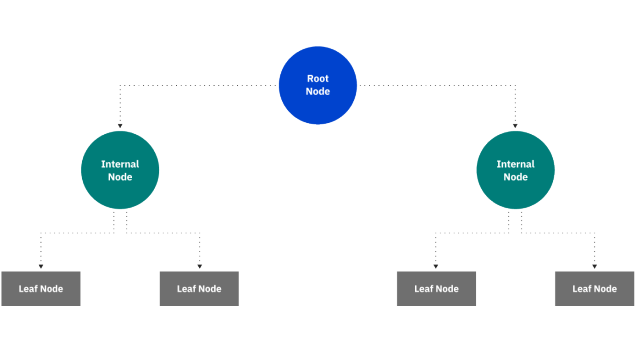
\includegraphics[width=0.75\textwidth]{098}
\end{center}
\caption{Decision tree structure.}
\label{fig:098}
\end{figure}
Given a training set \(D_n=\{z_1,...,z_n\}\), the set \(T\) of all the possible decision trees, find \(f_{t^*}\), that corresponds to the optimal tree, where 
\begin{equation}
    t^* \in arg\ \min_{t \in T} E(f_t;D_n)
\end{equation}
The optimization problem is easy if we don't impose constraints (e.g. most compact tree), a solution can be found using a simple, greedy strategy. Otherwise, the complexity class could be NP-hard. Hereafter, we will assume:
\begin{equation}
    E(f_t; D) = \frac 1 {|D|} \sum_{z \in D} l(f;z)
\end{equation}
That means that the empirical error of our training set can be computed by the normalized sum of the pair-wise losses.

Fix a set of leaf predictions \(H_\text{leaf} \subset F_\text{task}\) (e.g., constant functions), that correspond to the number of classes. Fix a set of possible split functions \(\Phi \subset \{L,R\}^X\). Define the tree-growing strategy that recursively partitions the training set and decides whether to grow leaves or non-terminal nodes. Finally, we stop when the final criteria is reached, and all the examples of the current training set are associated to the same class. 

\subsubsection{Growing a leaf}
Growing a leaf means to find a way to know if the current training set are associated to the same class. Formally, given \(D = \{z_1,...,z_n\}\) the training set reaching the node. The optimal leaf predictor, that minimizes the local error, can be computed as:
\begin{equation}
    h_D^* \in arg \min_{h \in H_\text{leaf}} E(h;D)
\end{equation}
The optimal error value is also called \textbf{impurity measure}, and tells us what is the probability of misclassifying an observation. Note that the lower the impurity, the better the split.
\begin{equation}
    I(D) = E(h_D^*; D)
\end{equation}
If some criterion is met we grow a leaf \(Leaf(h_D^*)\), for example:
\begin{itemize}
    \item 
    Purity \(I(D) < E\);
    \item
    Minimum cardinality \(|D| < k\);
    \item
    Others...
\end{itemize}

\subsubsection{Growing a node}
Given the set of all the possible routing functions \(\Phi\), and the set of training samples \(D\); if no stopping criterion is met, find the optimal split function, by minimizing the impurity function of our training set.
\begin{equation}
    \phi_D^* \in arg\ \min_{\phi \in \Phi} I_\phi (D)
\end{equation}
The impurity \(I_\phi(D)\) of a split function \(\phi\) given a training set \(D\) is computed in terms of the impurity of the split data:
\begin{align}
    I_\phi(D) &= \sum_{d \in \{L,R\}} \frac {|D_d^\phi|} {|D|} I(D_d^\phi)\\
    D_d^\phi &= \{(x,y) \in D; \phi(x) = d\}
\end{align}
Note that the impurity of a split function is the lowest training error that can be attained by a tree consisting of a root and two leaves.

Now, we finally grow a node \(Node(\phi^*, t_L, t_R)\), where \(\phi^*\) is the optimal split. \(t_L\) and \(t_R\) are obtained by recursively applying the learning algorithm to the associated training set splits.

In a nutshell:
\begin{equation}
    \text{Grow}(D)=\begin{cases}
        Leaf(h_D^*)                                                &\text{if stopping criterion met}\\
        Node(\phi_D^*, \text{Grow}(D_L^*), \text{Grow}(D_R^*))     &\text{otherwise}
    \end{cases}
\end{equation}

\subsection{About split selection}
Sometimes the selection of the best split function is not given in terms of minimizing the impurity of the split, but in the equivalent maximization of information gain, which is given by:
\begin{equation}
    \Delta_\phi(D)=I(D)-I_\phi(D)
\end{equation}
Information gain is non-negative, i.e. \(\Delta_\phi(D) \geq 0\) for any \(\phi \in \{L,R\}^X\) and any training set \(D \subset X \times Y\). So, the impurity will never increase for any randomly chosen split.

\subsection{Leaf predictions}
The leaf rediction provides a solution to a simplified problem involving only data reaching the leaf. This solution can be an arbitrary function \(h \in F_\text{task}\) but in practice we restrict it to a subset \(H_\text{leaf}\) of simple ones. 

The simplest predictor one can construct is a function returning a constant (e.g. a prefixed class label). The set of all possible constant functions can be written as:
\begin{equation}
    H_\text{leaf} = \bigcup_{y \in Y} \{y\}^X
\end{equation}

\section{Impurity measures for classification}
The impurity is a measure to take care of, because it can completely change the construction of the decision tree: the decision trees decide whether a node can be an inner node or a leaf, based on the impurity measure, which makes critical the decision of the kind of measure to choose for the model.

In the case of classification, we have an output space \(Y = \{c_1,...,c_k\}\) and a training set \(D \subset X \times Y\), that is the cartesian product of the input space and output space. Let \(D^y = \{(x,y') \in D : y = y'\}\) denote the subset of training samples in \(D\) with class label \(y\). 

Consider the following error function:
\[E(f;D) = \frac 1 {|D|} \sum_{z \in D} l(f;z)\]
With respect to this equation, we can now have different loss function that can lead us to completely different error functions.

\subsubsection{Classificationn error}
If the loss function is \(l(f;(x,y)) = 1_{f(x) \neq y}\), meaning that it is \(1\) if the condition \(f(x) \neq y\) is verified, and \(H_\text{leaf} = \cup_{y \in Y} \{y\}^X\), where \(H_\text{leaf}\) is the set of all the leaves, then the impurity measure is the misclassification rate, or \textbf{classification error}:
\begin{equation}
    I(D) = 1 - max_{y\in Y} \frac {|D^Y|} {|D|}
\end{equation}

\subsubsection{Gini Impurity}
If the set of all the leaves is \(H_\text{leaf} = \cup_{\pi \in \Delta(Y)} \{\pi\}^X\), that is the constaint label distribution as leaf prediction, and the loss function is \(l(f;(x,y)) = \sum_{c \in Y} [f_c(x) - 1_{c=y}]^2\), then the impurity measure is the \textbf{Gini impurity}:
\begin{equation}
    I(D) = 1 - \sum_{y \in Y} \left( \frac {|D^y|} {|D|} \right) ^2
\end{equation}
The Gini impurity is a measure of how often a randomly chosen element from the set would be incorrectly labeled if it was randomly labeled according to the distribution of labels in the subset.

\subsubsection{Entropy}
In data science, the entropy is used as a way to measure the level of disorder, and can give a deterministic value of how mixed a column is, that is the information. The more mixed our set of all leaves is, the higher the entropy, so we can use the formula to determine how good the split has been.

If the set of all the leaves is again defined as the constant label distribution \(H_\text{leaf} = \cup_{\pi \in \Delta(Y)} \{\pi\}^X\), and the loss function is defined as \(l(f;(x,y)) = -\log f_y(x)\) then the impurity measure is the \textbf{entropy}:
\begin{equation}
    I(D) = - \sum_{y \in Y} \frac {|D^y|} {|D|} \log \frac {|D^y|} {|D|}
\end{equation}

\section{Impurity measures for regression}
In the case of regression, we have the output space \(Y \subset \mathbb(R)^d\), and \(D \subset X \times Y\). If \(l(f;(x,y)) = ||f(x) - y||^2\), and \(H_\text{leaf}=\cup_{y \in Y} \{y\}^X\), then the impurity measure is the \textbf{variance} associated to all the points in the  training set:
\begin{equation}
    I(D) = \frac 1 {|D|} \sum_{(x,y) \in D} ||x - \mu_D||^2
\end{equation}
where \(\mu_D = \frac 1 {|D|} \sum_{(x,y) \in D} x\) is the \emph{mean} of all the points in the training set.

\section{Split functions}
A data point \(x \in X\) could be \(d\)-dimensional with each dimension taking heterogeneous types of values (discrete, continuous) and have a total ordering or not (ordinal or nominal).

The split function \(\phi \in \{L,R\}^X\) determines wheter a data point \(x \in X\) should move left (\(\phi(x) = L\)) or right (\(\phi(x) = R\)). The possible split functions are restricted to some predefined set \(\Phi \subset \{L,R\}^X\) depending on the nature of the feature space. The prototypical split function for a \(d\)-dimensional input first selects one dimension and then applies a \(1\)-dimensional splitting criterion.

\subsection{Discrete nominal features}
Assume discrete nominal features taking values in \(K\) (e.g. colors, marital status, etc.). The split function can be implemented given a partition of \(K\) into \(K_R\) and \(K_L\), associated to different partitions of the tree.
\begin{equation}
    \phi(x) = \begin{cases}
        L \qquad &\text{if }x \in K_L \\
        R \qquad &\text{if }x \in K_R \\
    \end{cases}
\end{equation}
Finding the optimal split requires testing \(2^{|K|-1}-1\) bi-partitions.

\subsection{Ordinal features}
Assume ordinal features, i.e. can be sorted (numbers, t-shirt sizes, etc.), taking values in \(K\). The split function can be implemented given a threshold \(r \in K\):
\begin{equation}
    \phi(x) = \begin{cases}
        L \qquad &\text{if }x \leq r \\
        R \qquad &\text{if }x > r \\
    \end{cases}
\end{equation}
If \(|K| \leq |D|\), finding the optimal split requires testing \(|K|-1\) thresholds. Otherwise, it requires sorting the input values in \(D\), where \(D\) is the training set reaching the node, and testing \(|D|-1\) thresholds.

\subsection{Oblique}
Sometimes it is convenient to split using multiple features at once. Such split functions work with continuous features and are called \textbf{oblique}, because can generate oblique decision boundaries. If \(x \in \mathbb{R}^d\) then the split function can be implemented given \(w \in \mathbb{R}^d\) and \(r \in \mathbb{R}\):
\begin{equation}
    \phi(x) = \begin{cases}
        L \qquad &\text{if }w^Tx \leq r \\
        R \qquad &\text{otherwise} \\
    \end{cases}
\end{equation}

\section{Overfitting}
Decision trees are \textbf{non-parametric models} with a structure that is determine by the data. As a result, they are flexible and can wasily fit the training set, but with high risk of \textbf{overfitting}. 

Standard techniques to improve generalization apply also to decision trees:
\begin{itemize}
    \item early stopping;
    \item regularization;
    \item data augmentations;
    \item complexity regularization;
    \item ensembling.
\end{itemize}

\subsection{Pruning}
Pruning is a data compression technique that reduces the size of decision trees by removing sections in the tree that are non-critical and redundant to classify instances. Pruning reduces the complexity of the final classifier, and hence improves predictive accuracy by the reduction of overfitting.

A common strategy is to grow the tree until each node contains a small number of instances then use pruning to remove nodes that do not provide additional information.

Pruning should reduce the size of a learning tree without reducing predictive accuracy as measured by a cross-validation set. There are many techniques for tree pruning that differ in the measurement that is used to optimize performance.

\section{Random forests}
Random forests are an ensemble learning method for classification, regression, and other tasks that operate by constructing a multitude of decision trees at training time. For classification tasks, the output of the random forest is the class selected by most trees. For regression tasks, the mean or average prediction of the individual trees is returned. Random forests correct for decision trees' habit of overfitting to their training set. They generally outperform decision trees, but their accuracy is lower than gradient boosted trees. However, data characteristics can affect their performance. 

If we build many trees, all of which work weel and overfit in different ways, we can reduce the amount of overfitting by averaging their results. This reduction in overfitting, while retaining the predictive power of the trees, can be shown using rigorous mathematics.

To implement this strategy, we need to build many decision trees. Each tree should do an acceptable job of predicting the target, and should also be different from the other trees. Random forests get their name from injecting randomness into the tree building to ensure each tree is different.

Split functions are optimized on randomly sampled features, or are sampled completely at random. This helps obtaining decorrelated decision trees. The final prediction of the forest is obtained by averaging the prediction of each tree in the ensemble \(Q = \{t_1,...,t_T\}\).
\begin{equation}
    f_Q(x) = \frac 1 T \sum_{j=1}^T f_t(x)
\end{equation}

\subsection{Algorithm}
\begin{algorithm}
\caption{Random Forest Learning}
\label{alg:perceptron}
\ForEach{$b \gets 1$ to $B$}{
    Draw a boostrap sample $\vec Z^*$ of size $N$ from the training data\;
    Grow a random-forest tree $T_b$ to the bootstrapped data\;
    \ForEach{terminal node $\in$ $T_b$}{
        \Repeat{minimum node size $n_\text{min}$ is reached}{
            Select $m$ variables at random from the $p$ variables\;
            Pick the best variable/split-point among the $m$\;
            Split the node into two daughter nodes\;
        }
    }
}
\Return{Output the ensemble of trees $T_b$}
\end{algorithm}

While random forests often achieve higher accuracy than a single decision tree, they sacrifice the intrinsic interpretability present in decision trees. They are very powerful, often work well without heavy tuning of the parameters, and don't require scaling of the data. Essentially, they share all of the benefits of decision trees, while making up for some of their deficiencies.

\begin{figure}[b!]
\begin{center}
    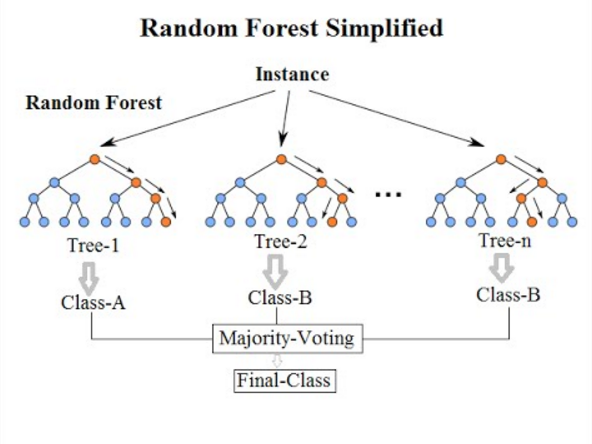
\includegraphics[width=.75\textwidth]{034}
\end{center}
\caption{Random forest classification example}
\label{fig:034}
\end{figure}

One reason to still use decision trees is if you need a compact representation of the decision making process. It is basically impossible to interpret tens or hundreds of trees in detail, and trees in random forests tend to be deeper than decision trees.

One application example of the random forest is a notable application in computer vision: the \textbf{kinect}.

\newpage
\begin{exercise}[topsep=20pt,itemsep=10pt]
    \ex Describe the decision trees. How does a decision tree work?
    \ex How does a decision tree infer?
    \ex[!] Describe the decision tree learning algorithm.
    \ex[!] How does a decision tree know when to grow a leaf and when to grow an inner node?
    \ex Describe the classification error, the Gini impurity, and the entropy.
    \ex Describe the split function for discrete nominal features, ordinal features.
    \ex What is the oblique? 
    \ex How can the overfitting problem solved? Describe the concept of pruning.
    \ex Describe the random forests. What are the differences with respect to decision trees?
    \ex[!] What are the advantages of random forests against decision trees?
\end{exercise}
% \chapter{Multi-class classification}

Multiclass classification is the problem of classifying instances into one of three or more classes. While many classification algorithms naturally permit the use of more than two classes, some are by nature binary algorithms; these can, however, be turned into multinomial classifiers by a variety of strategies.

Most of the real-world applications involve multiclass classification, for example:
\begin{itemize}[topsep={0pt}, partopsep={0pt}]
    \item document classification,
    \item handwriting recognition,
    \item face recognition,
    \item sentiment analysis,
    \item autonomous vehicles,
    \item emotion recognition.
\end{itemize}

We will see that it's relatively easy to think of a binary classifier as a \emph{black box}, which can be reused for solving these more complex problems. This is a very useful abstraction, since it allows us to reuse knowledge, rather than having to build new learning models and algorithms from scratch.

Formally, given an input space \(X\) and a number of classes \(K\), an unknow distribution \(D\) over \(X \times [K]\), and a training set \(D'\) sampled from \(D\). The multiclass classification computes a function \(f\) minimizing \(\mathbb{E}_{(x,y)\sim D} [f(x) \neq y]\).

\section{Extension from binary}

This section discusses strategies of extending the existing binary classifiers to solve multi-class classification problems.

\subsection{\(k\)-nearest neighbours}
\(k\)-nearest neighbors is considered among the oldest non-parametric classification algorithms. To classify an unknown example, the distance from that example to every other training example is measured. The \(k\) smallest distances are identified, and the most represented class by these \(k\) nearest neighbours is considered the output class labe.

\subsection{Decistion trees}
Decision tree learning is a powerful classification technique. The tree tries to infer a split of the training data based on the values of the available features to produce a good generalization. The algorithm can naturally handle binary or multiclass classification problems. The leaf nodes can refer to any of the \(K\) classes concerned.

\subsection{Perceptron}
It is hard to separate three or more classes with just one line, so the perceptron algorithm need some changes to fit the multiclass classification problem.

Using a binary classifier as a black box, can reduce the task of multicalss classification to the binary case? There are multiple ways to decompose the multiclass prediction into multiple binary decisions. Two approaches are:
\begin{itemize}
    \item One-versus-all,
    \item All-versus-all.
\end{itemize}

\begin{figure}[t]
\begin{center}
    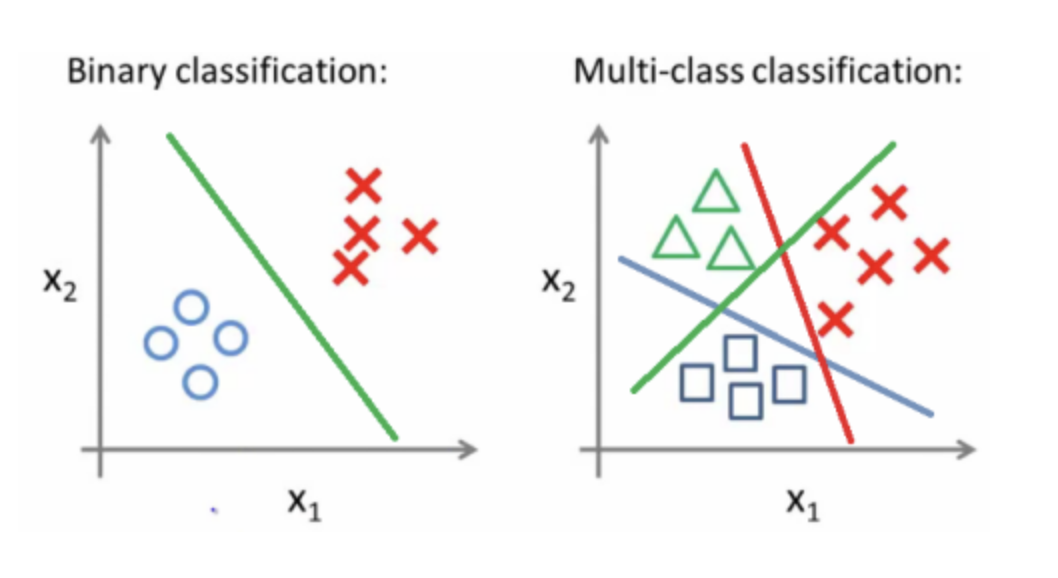
\includegraphics[width=.75\textwidth]{035}
	\vspace*{-35pt}
\end{center}
\caption{Binary classification vs Multiclass classification}
\label{fig:035}
\end{figure}

\section{One vs All}
A very common approach is the \textbf{one versus all} technique. To perform OVA, you train \(K\)-many binary classifiers \(f_1,...,f_K\). Each classifier sees all of the training data. Classifier \(f_i\) receives all examples labeled class \(i\) as positives and all other examples as negatives.

At test time, whichever classifier predicts positive wins, with ties broken randomly.

\begin{algorithm}
    \caption{OneVersusAllTrain($D^\text{multiclass}$, $BinaryTrain$)}
    \label{alg:ovatrain}
\For{$i \gets 1,...,K$}{
	$D^\text{bin} \gets$ relabel $D^{multiclass}$ so class $i$ is positive, and class $\neg i$ is negative\;
	$f_i \gets BinaryTrain(D^\text{bin})$\;
}
\Return{$f_1,...,f_K$}
    \end{algorithm}

In the testing procedure, the prediction of the \(i\)th classifier is added to the overall score for class \(i\). Thus, if the prediction is positive, class \(i\) gets a vote; if the prediction is negative, every one else (implicitly) gets a vote.

	\begin{algorithm}
		\caption{OneVersusAllTest($f_1,...,f_K$, $x$)}
		\label{alg:ovatest}
		$score \gets \langle 0,0,...,0 \rangle$\;
	\For{$i \gets 1,...,K$}{
		$y \gets f_i(x)$\;
		$score_i \gets score_i + y$\;
	}
	\Return{$argmax_k\ score_k$}
		\end{algorithm}

OVA is quite natural and easy to implement. It also works very well in practice, so long as you do a god job choosing a good binary classification algorithm tuning its hyperparameters well.

Its weakness is that it can be somewhat brittle. Intuitively, it is not particularly robus to errors in the underlying classifiers. If one classifier makes a mistake, it is possible that the intire prediction is erroneous. In fact, it is entirely possible that \emph{none} of the \(K\) classifier predicts positive (which is actually the worst scenario)!

\section{All vs All}
To develop alternative approeaches, a useful way to think about turning multiclass classification problems into binary classification problems is to think of them like torunaments. You have \(K\) teams entering a tournament, but unfortunately the sport they are playing only allows two to compete at a time. 

One natural approach is to have every team compete against every other team. The team that wins the majority of its matches is declared the winner. This is the \textbf{all versus all} approach.

The most natural way to think about it is as training \(K \choose 2\) classifiers. Say \(f_{ij}\) for \(1 \leq i < j \leq K\) is the classifier that pits class \(i\) against class \(j\). This classifier receives all of the class \(i\) examples as positive and all of the class \(j\) examples as negative. When a test point arrives, it is run through all \(f_{ij}\) classifiers. Every time \(f_{ij}\) predicts positive, class \(i\) gets a point; otherwise, class \(j\) gets a point. After running all \(K \choose 2\) classifiers, the class with the most votes wins.

\begin{algorithm}
    \caption{AllVersusAllTrain($D^\text{multiclass}$, $BinaryTrain$)}
    \label{alg:avatrain}
	$f_{ij} \gets \emptyset, \forall 1 \leq i < j \leq K$\;
\For{$i \gets 1,...,K-1$}{
	$D^\text{pos} \gets$ all $x \in D^\text{multiclass}$ labeled $i$\;
	\For{$j \gets i+1,...,K$}{
		$D^\text{neg} \gets$ all $x \in D^\text{pos}$ labeled $j$\;
		$D^\text{bin} \gets \{(x, +1) : x \in D^\text{pos}\} \cup \{(x, -1) : x \in D^\text{neg}\}$\;
		$f_{ij} \gets BinaryTrain(D^\text{bin})$\;
	}
}
\Return{all $f_{ij}$}
    \end{algorithm}

	\begin{algorithm}
		\caption{AllVersusAllTest(all $f_{ij}$, $x$)}
		\label{alg:avatest}
		$score \gets \langle 0, 0, ..., 0 \rangle$\;
		\For{$i \gets 1,...,K-1$}{
			\For{$j \gets i+1,...,K$}{
			$y \gets f_{ij}(x)$\;
			$score_i \gets score_i + y$\;
			$score_j \gets score_j - y$\;
			}
		}
	\Return{$argmax_k\ score_k$}
		\end{algorithm}

\section{OVA vs AVA}
In terms of train time, AVA learns more classifiers, however, they are trained on much smaller data, and this tends to make it faster if the labels are equally balanced.

In terms of test time, AVA has more classifiers, so often is slower.

Furthermore, AVA trains on more balanced data sets, and test with more classifiers, therefore has more chances for errors.

If using a binary classifier, the most common thing to do is OVA. Otherwise, use a classifier that allows for multiple labels, for example decision trees and \(k\)-NN work reasonably well, but other more sophisticated methods work better.

\section{Evaluation}

Selecting the best metrics for evaluating the performance of a given classifier on a certain dataset is guided by a number of consideration including the class-balance and expected outcomes. One particular performance measure may evaluate a classifier rom a single perspective and often fail to measure others. Consequently, there is no unified metric to measure the generalized performance of a classifier.

Two methods, \textbf{micro-averaging}, and \textbf{macro-averaging} are used to extract a single number for each of the precision, recall and other metrics across multiple classes.

A macro-average calculates the metric autonomously for each class to calculate the average. 

In contrast, the micro-average calculates average metric from the aggregate contributions of all classes. Micro-average is used in unbalanced datasets as this method takes the frequency of each class into consideration. The micro average precision, recall, and accuracy scores are mathematically equivalent.

\subsection{Confusion matrix}

\begin{figure}[t]
\begin{center}
	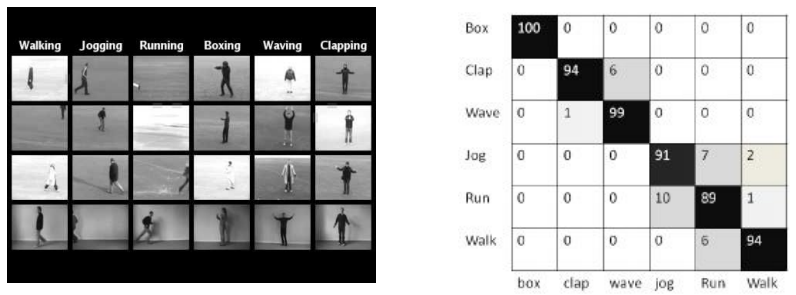
\includegraphics[width=\textwidth]{036}
	\vspace*{-25pt}
\end{center}
\caption{Confusion matrix example}
\label{fig:036}
\end{figure}
A confusion matrix shows the combination of the actual and predicted classes. Each row of the matrix represents the instances in a predicted class, while each column represents the instances in an actual class. It is a good measure of whether models can account for the overlap in class properties and understand which classes are most easily confused.

% \chapter{Gradient Descent}

Gradient descent is a first-order iterative optimization algorithm for finding a local minimum of a differentiable function. The idea is to take repeated steps in the opposite direction of the gradient of the funciont at the current point, because this is the direction of steepest descent. Conversely, stepping in the direction of the gradient will lead to a local maximum of that function; the preocedure is then known as \textbf{gradient ascent}.

\section{Notation}
Let's introduce some convenient notation. The indicator function is a function for turning \texttt{true} and \texttt{false} answers into numbers or counts:
\begin{align}
    1[x] = \begin{cases}
        1\qquad &\text{if }x=\texttt{true}\\
        0\qquad &\text{if }x=\texttt{false}\\
    \end{cases}
\end{align}
We use a \textbf{vector notation}. We represent an example \(f_1,f_2,...,f_m\) as a single vector, \(\vec{x}\). Similarly, we can represent the weight \(w_1,w_2,...,w_m\) as a single vector, \(\vec{w}\).

The dot-product between two vectors \(\vec{a}\) and \(\vec{b}\) is defined as:
\begin{align}
    a \cdot b = \sum_{j=1}^m a_jb_j
\end{align}

\section{The optimization framework for Linear Models}
We have already seen the perceptron as a way of finding a weight vector \(\vec{w}\) and bias \(b\) that do a good job of separating positive training examles from negative training examples. The goal of the perceptron was to find a separating hyperplane for some training data set. Not all data sets are linearly separable. In the case that your training data \emph{isn't} linearly separable, you might want to find the hyperplane that makes the \emph{fewest errors} on the training data. We can write this down as a formal mathematics optimization problem as follows:
\begin{align}
    \label{eqn:optimization}
    \min_{w,b} \sum_n 1[y_n(\vec{w} \cdot \vec{x} + b) > 0]
\end{align}
The objective function is the thing we are trying to minimize. In this case, the objective function is simply the \textbf{error rate} of the linear classifier parametrized by \(\vec{w}\), \(b\).

We know that the perceptron algorithm is guaranteed to find parameters for this model if the data is linearly separable. In other words, if the optimum of \ref{eqn:optimization} is zero, then the perceptron will efficiently find parameters for this model.

\section{Convex Surrogate Loss Functions}
There are two equivalent definitions of a convex function. The first is that it's second derivative is always non-negative. The second definition is that any chord of the function lies above it.

Convex functions are nice because they are easy to minimize. This leads to the idea of \textbf{convex surrogate loss functions}. Since zero/one loss is hard to optimize, we want to optimize something else, instead. Since convex functions are easy to optimize, we wanto to approximate zero/one loss with a convex function This approximating function will be called a \textbf{surrogate loss}. The surrogate losses we construct will always be \emph{upper bounds} on the true loss function: this guarantees that if you minimize the surrogate loss, you are also pushing down the real loss.

There are four common surrogate loss functions, each with their own properties:
\begin{align}
    \text{Zero/one}& \qquad l^{(0/1)}(y,\hat{y}) = 1[y\hat{y} \leq 0] \\
    \text{Hinge}& \qquad l^\text{(hin)}(y,\hat{y}) = \max\{0,1-y\hat{y}\} \\
    \text{Logistic:}& \qquad l^\text{(log)}(y,\hat{y}) = \frac 1 {\log 2} \log (1 + exp [-y\hat{y}]) \\
    \text{Exponential:}& \qquad l^\text{(exp)}(y,\hat{y}) = exp[-y\hat{y}] \\
    \text{Squared:}& \qquad l^\text{(sqr)}(y,\hat{y}) = (y-\hat{y})^2
\end{align}

There are two big differences in these loss functions. The first is how \emph{upset} they get by erroneous predictions. In the case of hinge and logistic loss, the growth of the function as \(\hat{y}\) goes negative is linear. For squared and exponential loss, it is super-linear. This means that exponential loss would rather get a few examples a little wrong than one example really wrong.
The other difference is how they deal with very confident correct predictions. Once \(y\hat{y}>1\), hinge loss does not care any more, byt logistic and exponential loss still think you can do better. On the other hand, squared loss thinks it's just as bad to predict \(+3\) on a positive example as it is to predict \(-1\) on a positive example.

\begin{figure}[t]
    \begin{center}
        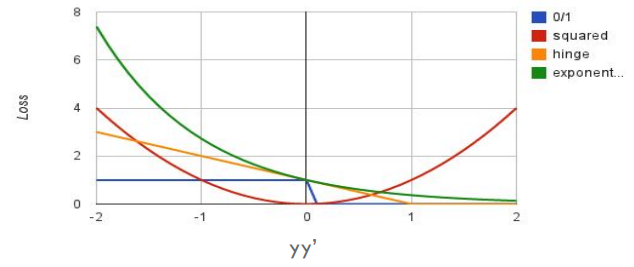
\includegraphics[width=\textwidth]{039}
        \vspace*{-25pt}
    \end{center}
    \caption{Surrogate loss functions}
    \label{fig:039}
    \end{figure}

\section{Gradients, math review}
A gradient is a multidimensional generalization of a derivative. Suppose you have a function \(f : \mathbb{R}^D \to \mathbb{R}\) that takes a vector \(\vec{x} = \langle x_1, x_2, ..., x_D \rangle \) as input and produces a scalar value as output.

You can differentiate this function according to any one of the inputs; for instance, you can compute \(\frac {\delta f} {\delta x_5}\) to get the derivative with respect to the fifth input. The \textbf{gradient} of \(f\) is just the vector consissting of the derivative \(f\) with respect to each of its input coordinates independently, and is denoted \(\nabla f\), or, when the input to \(f\) is ambiguous, \(\nabla_x f\). This is defined as:
\begin{align}
    \nabla_x f = \langle \frac{\delta f}{\delta x_1}, \frac{\delta f}{\delta x_2}, ..., \frac{\delta f}{\delta x_D} \rangle
\end{align}
For example, consider the function \(f(x_1,x_2,x_3) = x_1^3+5x_1x_2-3x_2x_3^2\). The gradient is:
\begin{align}
    \nabla_x f = \langle 3x_1^2 + 5x_2, 5x_1-3x_3^2, -6x_2x_3 \rangle
\end{align}
Note that if \(f : \mathbb{R}^ \to \mathbb{R}\), thent \(\nabla f : \mathbb{R}^D \to \mathbb{R}^D\). If you evaluate \(\nabla f(x)\), this will give you the gradient at \(\vec{x}\), a vector in \(\mathbb{R}^D\). This vector can be interpreted as the direction of \textbf{steepest ascent}: namely, if you were to traver an infinitesimal amount in the direction of the gradient, you would go uphill the most.

\section{Optimization with gradient descent}
Suppose you are trying to find the maximum of a function \(f(\vec{x})\). The optimizer maintains a current estimate of the parameter of interest, \(\vec{x}\). At each step, it measures the \textbf{gradient} of the function it is trying to optimize. This measurement occurs at the current location, \(\vec{x}\). Call the gradient \(\vec{g}\). It then takes a step in the direction of the gradient, where the size of the step is controlled by a parameter \(\eta\). The complete step is \(\vec{x} \gets \vec{x} + \eta \vec{g}\). This is the basic idea of \textbf{gradient ascent}.

\begin{wrapfigure}{l}{0.25\textwidth}
\begin{center}
    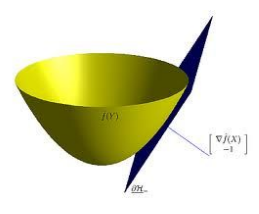
\includegraphics[width=0.25\textwidth]{038}
    \caption{Convex function}
	\vspace*{-40pt}
\end{center}
\label{fig:038}
\end{wrapfigure}

The opposite of gradient ascent is \textbf{gradient descent}. All of our learning problems will be framed as \emph{minimization} problems (trying to reach the bottom of a ditch, rather than the top of a hill). Therefore, descent is the primary approach you will use. One of the major conditions for gradient ascent being able to find the true, \textbf{global minimum}, of its objective function is convexity. Without convexity, all is lost.

\subsection{Algorithm}
\begin{algorithm}
    \caption{GradientDescent($F$, $K$, $\eta_1, ..., \eta_K$)}
    \label{alg:gradient_descent}
$\vec{z}^{(0)} = \langle 0,0,...,0 \rangle $\;
\For{$k \gets 1,...,K$}{
    $\vec{g}^{(k)} \gets \nabla_{\vec{z}} F |_{\vec{z}^{\,(k-1)}}$\;
    $\vec{z}^{(k)} \gets \vec{z}^{\,(k-1)} - \eta^{(k-1)} \vec{g}^{\,(k)}$\;
}
\Return{$\vec{z}^{\,(K)}$}
\end{algorithm}
The function takes as argument the function \(F\) to be minimized, the number of iterations \(K\) to run and a sequence of learning rates \(\eta_1, ..., \eta_K\). 

The only real work you need to do to apply a gradient descent method is be able to compute derivatives. Suppose we choose the exponential loss function. We are interested on how much we want to move in the error direction at each iteration: namely, we are interested on the value of \(\frac \delta {\delta w_i} l(z)\).
\begin{align}
    \label{eqn:loss_derivative}
    \frac {\delta l} {\delta w_j} &= \frac \delta {\delta w_j} \sum_{i=1}^n \exp (-y_i (w \cdot x_i + b)) \\
    &= \sum_{i=1}^n \exp (-y_i (w \cdot x_i + b)) \frac \delta {\delta w_j} -y_i (w \cdot x_i + b)
\end{align}
Now, in order to make it more clear, let's expand the operations for the member \(- \frac \delta {\delta w_i} y_i(w \cdot x_i + b)\).
\begin{align*}
    - \frac {\delta l} {\delta w_j} -y_j (w \cdot x_j + b) &= - \frac \delta {\delta w_j} y_j (\sum_{j=1}^m w_j x_{ij} + b)\\
    &= -\frac \delta {\delta w_j} y_j (w_1 x_{i1} + w_2 x_{i2} + ... + w_m x_{im} + b) \\
    &= -\frac \delta {\delta w_j} (y_j w_1 x_{i1} + y_j w_2 x_{i2} + ... + y_j w_m x_{im} + y_j b) \\
    &= -y_j x_{ij}
\end{align*}
Let's now take this result and return to expand the equation \ref{eqn:loss_derivative}.
\begin{align}
    \frac \delta {\delta w_j} &= \sum_{i=1}^n \exp (-y_i (w \cdot x_i + b)) \frac \delta {\delta w_j} -y_i (w \cdot x_i + b) \\
    &= \sum_{i=1}^n -y_i x_{ij} \exp (-y_i (w \cdot x_i + b))
\end{align}
That means that for each example \(x_i\), the exponential update rule is:
\begin{equation}
    w_j = w_j + \eta y_i x_{ij} exp(-y_i (w \cdot x_i + b))
\end{equation}
If you remember from \ref{alg:perceptron} perceptron algorithm, there is a similarity: \(w_i \gets w_i + f_i*label\). In practice: \(w_j \gets w_j + x_{ij} y_i c\), where \(c = \eta exp(-y_i (w \cdot x_i + b))\).
% \chapter{Regularization}
In our learning objectice, we had a erm correspond to the zero/one loss on the training data, plus a \textbf{regularizer} whose goal was to ensure that the learned function did not overfit. If you replace to zero/one loss with a surrogate loss, you obtain the following objective:
\begin{equation}
    \min_{w,b} \sum_n l(y_n, \vec{w} \cdot \vec{x}_n + b) + \lambda R(\vec{w},b)
\end{equation}
From the discussion of surrogate loss function, we would like to ensure that \(R\) is convex. Otherwise, we will be back to the point where optimization becomes difficult. Beyond that, a common desire is that the components of the weight vecotr should be small. This is a form of \textbf{inductive bias}.

\section{Regularizers}

If \(w_i\) is reasonably small, this is unlikely to have much of an effect on the classification decision. On the other hand, if \(w_i\) is large, this could have a large effect. 
Another way to say the same thing is to look at the derivative of the predictions as a function of \(w_i\). The derivative of \(\vec{w} \cdot \vec{x} + b\) with respect to \(w_i\) is:
\begin{equation}
    \frac {\delta [\vec{w} \cdot \vec{x} + b]} {\delta w_i} = \frac {\delta [\sum_d w_d x_d + b]} {\delta w_i} = x_i
\end{equation}
Interpreting the derivative as the rate of change, we can see that the range of change of the prediction funcion is proportional to the individual weights. So if you want the function to change slowly, you want to ensure that the weights stay small.

One way to accomplish this is to simply use the norm of the weight vector. Namely \(R^\text{(norm)}(\vec{w},b) = ||\vec{w}|| = \sqrt{\sum_d w_d^2}\). This function is convex and smooth, which makes it easy to minimize.

An alternative to using the sum of squared weights is to use the sum of absolute weights: \(R^\text{(abs)}(\vec{w},b) = \sum_d |w_d|\).

\section{\(p\)-norm}
The line of thinking leads to the general concept of \(p\)-norms. This is a family of norms that all have the same generalflavor. We write \(||\vec{w}||_p\) to denote the \(p\)-norm of \(\vec{w}\).
\begin{equation}
    ||\vec{w}||_p = R(\vec{w},b) = \sqrt[p]{\sum_{w_j} |w_j|^p}
\end{equation}
You can check that the 2-norm exactly corresponds to the usual Euclidean norm, and the 1-norm corresponds to the absolut regularizer described above.

\begin{wrapfigure}{r}{0.25\textwidth}
    \begin{center}
        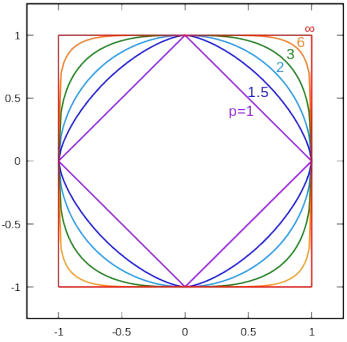
\includegraphics[width=0.25\textwidth]{040}
        \caption{\(p\)-norms visualized}
        \vspace*{-40pt}
    \end{center}
    \label{fig:040}
    \end{wrapfigure}

When \(p\)-norms are used to regularize weight vectors, the interting aspect is how they trade-off multiple features. To see the behavior of \(p\)-norms in two dimensions, we can plot their \textbf{contour}.

Figure~\ref{fig:040} shows the contours for the same \(p\)-norms in two dimensions. Each line denotes two-dimensional vectors to which this norm assignes a total value of 1. By changing the value of \(p\), you can interpolate between a square, down to a circle.

In general, smaller values of \(p\) prefer sparser vectors. You can see this by noticing that the contours of small \(p\)-norms stretch out along the axes.

\section{Minimizing with a regularizer}
We know how to solve convex minimization problems using gradient descent.
\begin{equation*}
    \min_{\vec{w},b} \sum_{i=1}^n loss(yy')
\end{equation*}
If we can ensure that the loss with the regularizer is convex, then we could still use gradient descent to solve convex minimization problems:
\begin{equation}
    \label{eq:gd_wit_regularizer}
    \min_{\vec{w},b} \sum_{i=1}^n loss(yy') + \lambda R(\vec{w})
\end{equation}
Equation~\ref{eq:gd_wit_regularizer} is convex as long as both the loss function and the regularizer are convex.

\subsection{Model-based machine learning}
There are the three step for the model-based machine learning:
\begin{itemize}
    \item Pick a model;
    \begin{equation}
        b + \sum_{j=1}^n w_jf_j = 0
    \end{equation}
    \item Pick a criteria to optimize, namely, pick the objective function;
    \begin{equation}
        \sum_{i=1}^n exp(-y_i(\vec{w} \cdot x_i + b)) + \frac \lambda 2 ||\vec{w}||^2
    \end{equation}
    \item Develop a learning algorithm;
    \begin{equation}
        \min_{\vec{w},b} \sum_{i=1}^n exp(-y_i(\vec{w} \cdot x_i + b)) + \frac \lambda 2 ||\vec{w}||^2
    \end{equation}
\end{itemize}
Note that the loss function penalizes examples where the prediction is different than the label; and regularizer penalizes large weights. This function is convex, thus is allowing us to use gradient descent.

\begin{align}
    \frac \delta {\delta w_j} \text{objective} &= \frac \delta {\delta w_j} \sum_{i=1}^n exp(-y_i(\vec{w} \cdot x_i + b))+ \frac \lambda 2 ||\vec{w}||^2\\
    &= -\sum_{i=1}^n y_i x_{ij} exp(-y_i(\vec{w} \cdot x_i + b)) + \lambda w_j\\
\end{align}
That means, that the gradient descent algorithm moves a small amount in a chosen dimension towards decreasing loss using the derivative.
\begin{align}
    w_j &= w_j - \eta \frac \delta {\delta w_j} (l(\vec{w}) + R(\vec{w},b))\\
    w_j &= w_j + \eta \sum_{i=1}^n y_i x_{ij} exp(-y_i(\vec{w} \cdot x_i + b)) - \eta \lambda w_j
\end{align}

\chapter{Support Vector Machines}

Support Vector Machine are a set of related supervised learning methods used for classification and regression. They belong to a family of generalized linear classifiers. In other terms, SVM is a classification and regression prediction tool that uses machine learning theory to maximize predictive accuracy while automatically avoiding overfit to the data. They became famous when, using pixel maps as input, they give accuracy comparable to sophisticated neural networks with elaborated features in a handwriting recognition task. It is also being used for many applications, such as hand writing analysis, face analysis and so fort, especially for pattern classification and regression based applications.

\begin{wrapfigure}{r}{0.35\textwidth}
    \begin{center}
        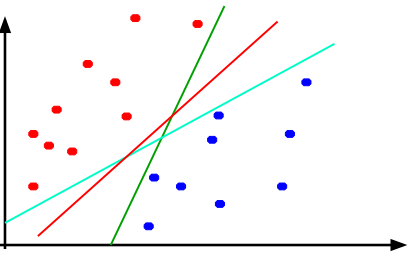
\includegraphics[width=0.35\textwidth]{041}
        \caption{Possible hyperplanes for linearly-separable data that shows the best solution (red middle line) compared to other possible solutions.}
        \label{fig:041}
        \vspace*{-10pt}
    \end{center}
\end{wrapfigure}

Let's start by thinking back to the original goal of linear classifiers: to find a hyperplane that separates the positive training examples from the negative ones. Figure~\ref{fig:041} shows some data and three potential hyperplane that separates the red training examples from the blue one. Which one do you like the best? Most likely you chose the red hyperplane. And most likely you chose it because it was furthest away from the closest training points. In other words, it has a large \textbf{margin}. The desire for hyperplanes with large margins is a perfect example of an inductive bias\footnote{\textbf{Inductive Bias} play an important role in the ability of models to generalize to the unseen data. A strong inductive bias can lead our model to converge to the global optimum, on the other hand, a weak inductive bias can cause the model to find only the local optima and be greatly affected by random changes in the initial states.}. Following this line of thinking leads us to the \textbf{Support Vector Machine} (SVM). this is simply a way of setting up an optimization problem that attempts to find a separating hyperplane with as large margin as possible. 

\section{Large margin classifiers}
The \textbf{margin} of a single data point is defined to be the distance from the data point to a decision boundary. Note that there are many distances and decision boundaries that may be appropriate for certain datasets and goals.

A \textbf{margin classifier} is a classifier which is able to give an associated distance from the decision boundary for each example. For instance, if a linear classifier is used, the distance of an example from the separating hyperplane is the margin of that example.

There are many hyperplanes that might classify the data. One reasonable choice of the best hyperplane is the one that represents the largest margin between the two classes. So we choose the hyperplane so that the distance from it to the nearest data point on each side is maximized. If such a hyperplane exists, it is known as the \textbf{maximum margin hyperplane} and the linear classifier it defines is known as a \textbf{maximum margin classifier}, or equivalently, the perceptron of optimal stability.
\begin{wrapfigure}{l}{0.4\textwidth}
    \begin{center}
        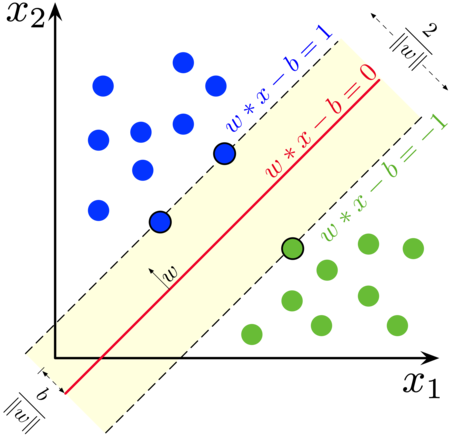
\includegraphics[width=0.35\textwidth]{042}
        \caption{Maximum-margin hyperplane and margins for an SVM trained with samples from two classes.}
        \label{fig:042}
    \end{center}
    \vspace*{-40pt}
\end{wrapfigure}
\subsection{Support vectors}
Support vectors are the elements of the training set that would change the position of the dividing hyperplane if removed. They are critical elements of the training set. Support vectors are observations that lie on the margin surrounding the data-separating hyperplane. Since the margin defines the minimum distance observations should have from the plane, the observations that lie on the margin impact the orientation and position of the hyperplane.

The problem of finding the optimal hyperplane is an optimization problem and can be solved by optimization techniques. For \(n\) dimensions, there will be at least \(n+1\) support vectors. We can see in Figure~\ref{fig:042} that there are 3 support vectors, 2 are of the blue class, and 1 of the green class.

\subsection{Maximizing the margin}
Given the hyperplane in Figure~\ref{fig:042}, we have the margins described by the equation \(\vec{w} \cdot \vec{x} - b = a\), where \(a=1\) for the blue margin, and \(a=-1\) for the green margin. The measure for the margin is defined by
\begin{equation}
    \frac {\vec{w} \cdot \vec{x}_i + b} {||\vec{w}||} = \frac 1 {||\vec{w}||}
\end{equation}

Our goal is now to maximize the margin, namely, to select the hyperplane with the largest margin where the points are classified correctly and outside the margin. Let's setup the problem as a constrained optimization problem, subject to \(y_i(\vec{w} \cdot \vec{x}_i + b) \geq 1 \quad \forall i\)
\begin{align}
    \max_{a,b} margin(\vec{w},b) &= \max_{w,b} \frac 1 {||\vec{w}||}\\
    &= \min_{w,b} ||\vec{w}||
\end{align}
Maximizing the margin is equivalent to minimize the norm of the weights (subject to separating constraints). The minimization criterion wants \(\vec{w}\) to be as small as possible, while the constraints make sure that the data is separable.

The \textbf{support vector machine problem} is a version of a \textbf{quadratic optimization problem}, which wants to minimize a quadratic function subject to a set of linear constraints.
\begin{align*}
    &\min_{\vec{w},b} ||\vec{w}||^2\\
    \text{subject to: } &y_i(\vec{w} \cdot \vec{x}_i + b) \geq 1 \quad \forall i
\end{align*}

\section{Soft margin classification}
For the very high dimensional problems common in classification, sometimes the data are linearly separable. But in general case they are not, and even if they are, we might prefer a solution that better separates the bulk of the data while ignoring a few weird noise. 

If the training set \(D\) is not linearly separable, the standard approach is to allow the fat decision margin to make a few mistakes (some points - outliers or noisy example - are inside or on the wrong side of the margin). We then pay a cost for each misclassified example, which depends on how far it is from meeting the margin requirements. To implement this, we introduce \emph{slack variables} \(\zeta_i\). A non-zero value for \(\zeta_i\) allows \(\vec{x}_i\) to not meet the margin requirement at a cost proportional to the value of \(\zeta_i\).

The formulation of the SVM optimization problem with slack variables is: Find \(\vec{w}\), \(b\) and \(\zeta_i \geq 0\) such that:
\begin{itemize}
    \item
    \(\frac 1 2 \vec{w}^T \vec{w} + C \sum_i \zeta_i\) is minimized
    \item
    and \(\forall \{(\vec{x}_i, y_i)\}\), \(y_i(\vec{w}^T \vec{x}_i + b) \geq 1 - \zeta_i\)
\end{itemize}
\begin{align*}
    &\min_{\vec{w},b} ||\vec{w}||^2\\ + C \sum_i \zeta_i
    \text{subject to: } &y_i(\vec{w} \cdot \vec{x}_i + b) \geq 1 - \zeta_i \quad \forall i,\ \zeta \geq 0
\end{align*}

The optimization problem is then a trading off how fat it can make the margin versus how many points have to be moved around to allow this margin. the margin can be less than 1 for a point \(\vec{x}_i\) by setting \(\zeta_i > 0\), but then one pays a penalty of \(C\zeta_i\) in the minimization for having done that. The sum of the \(\zeta_i\) gives an upper bound on the number of training errors.

\begin{figure}[h!]
    \centering
    \begin{subfigure}{.4\textwidth}
        \centering
        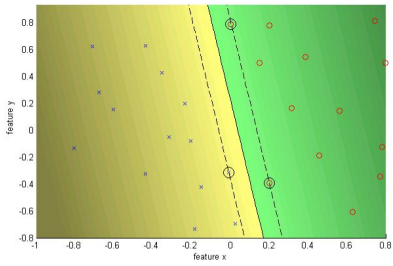
\includegraphics[width=1\textwidth]{043}
        \caption{\(C = \infty\) hard margin}
    \end{subfigure}
    \begin{subfigure}{.4\textwidth}
        \centering
        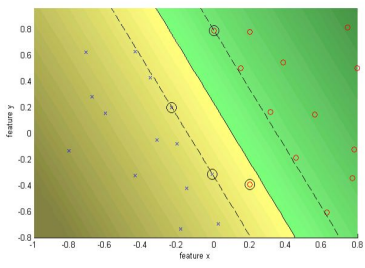
\includegraphics[width=1\textwidth]{044}
        \caption{\(C=10\) soft margin}
    \end{subfigure}
    \caption{Hard margin vs soft margin example.}
\end{figure}

Soft-margin SVMs minimize training error traded off against margin. The parameter \(C\) is a \emph{regularization term}, which proivdes a way to control overfitting: small \(C\) allows constraints to be easily ignored (large margin); large \(C\) makes constraints hard to ignore (narrow margin). If \(C = \infty\) enforces all constraints: \textbf{hard margin}. The slack variable can have two different values:
\begin{align}
    \zeta_i &= \begin{cases}
        0 &\text{if } y_i(\vec{w} \cdot \vec{x}_i + b) \geq 1\\
        1-y_i(\vec{w} \cdot \vec{x}_i + b) &\text{otherwise}\\
    \end{cases}\\
    &=\max(0, 1-y_i(\vec{w} \cdot \vec{x}_i + b))\\
    &=\max(0,1-yy')
\end{align}
Note that the last equality is the \textbf{hinge loss}, that is actually our loss, so we can rewrite our optimization problem as follows
\begin{equation}
    \min_{\vec{w},b} ||\vec{w}||^2 + C \sum_i \max(0,1-y_i(\vec{w} \cdot \vec{x}_i + b))
\end{equation}
That looks like the expression:
\begin{equation}
    arg \min_{\vec{w},b} \sum_i^n l(yy') + \lambda R(\vec{w} b)
\end{equation}

\section{Non linearly separable data}
We have gone though the understanding of \textbf{Support Vectors} and \textbf{Margins}. Then used the concepts to build the objective functions for soft margin classifier. We have have also learned the objective function, that is defined as \textbf{Primal Problem}. However our final goal is to solve non-linear SVM, where primal problem is not helpful, we need a procedure that increases the number of features in order to make our data linearly separable.

\subsubsection{Classes of Optimization Problems}
Let's revise some classes of optimization problems, in order to see where does the support vector machine objective function locate.

% paragraph  (end)
\paragraph{Linear Programming (LP)}
We have a linear problem, with linear constraints.
\begin{align*}
    &\min_{\vec{x}} \vec{c}^T \vec{x}\\
    \text{s.t. } &\vec{A} \vec{x} = b, \quad \vec{x} \geq 0
\end{align*}

\paragraph{Quadratic Programming (QP)}
We have a quadrative objective and linear constraints. It is convex if \(Q\) is positive semidefinite.
\begin{align*}
    &\min_{\vec{x}} \vec{c}^T \vec{x} + \frac 1 2 \vec{X}^T Q \vec{x}\\
    \text{s.t. } &\vec{A}\vec{x} = b, \quad C\vec{x} \geq d
\end{align*}

\paragraph{Nonlinear Programming (NLP)}
In general it is not convex.
\begin{align*}
    &\min_{\vec{x}} f(\vec{x})\\
    \text{s.t. } &g(\vec{x}) = 0, \quad h(\vec{x}) \geq 0
\end{align*}

\subsection{Dual problem}
In mathematical optimization theory, duality means that optimization problems may be viewed from either of two perspectives, the primal problem or the dual problem. The solution to the dual problem provides a lower bound to the solution of the primal (minimization) problem.

Quadratic optimization problems are a well-known class of mathematical programming problems for which several algorithms exist. One possible solution involves constructing a dual problem where a Lagrange multiplier \(\alpha_i\) is associated with every inequality constraint in the primal problem:

Find \(\alpha_1, ..., \alpha_n\) such that \(\sum_i \alpha_i - \frac 1 2 \sum_i \sum_j \alpha_i \alpha_j y_i y_j \vec{x}_i^T \vec{x}_j\) is maximized and
\begin{itemize}
    \item
    \(\sum_i \alpha_i y_i = 0\)\\
    \item
    \(\alpha_i \geq 0,\ \forall i\)
\end{itemize}

Given a solution \(\alpha_1...\alpha_n\) to the dual problem, the solution to the primal is:
\begin{align*}
    \vec{w} &= \sum_i \alpha_i y_i \vec{x}_i\\
    b &= y_k - \sum_i \alpha_i y_i \vec{x}_i^T \vec{x}_k \text{ for any } \alpha_k > 0
\end{align*}
Each non-zero \(\alpha_i\) indicates that the corresponding \(\vec{x}_i\) is a support vector. Then the classifying function is:
\begin{equation}
    f(\vec{x}) = \sum_i \alpha_i y_i \vec{x}_i^T \vec{x} + b
\end{equation}
The solution relies on an inner product between the test point \(\vec{x}\) and the support vectors \(\vec{x}_i\). Also solving the optimization problem involves the computing of the inner products between all training points.

Dual problem is similar in the non separable case, but notice the constraints.

Find \(\alpha_1...\alpha_N\) such that \(\sum_i \alpha_i - \frac 1 2 \sum_i \sum_j \alpha_i \alpha_j y_i y_j \vec{x}_i^T \vec{x}_j\) is maximized and
\begin{itemize}
    \item \(\sum_i \alpha_i y_i = 0\)\\
    \item \(0 \geq \alpha_i \geq C\) for all \(\alpha_i\)
\end{itemize}
Again, \(\vec{x}_i\) with non-zero \(\alpha_i\) represent support vectors.

\subsection{Kernel trick}
Suppose now that we would like to learn a nonlinear classification rule which corresponds to a linear classification rule for the transformed data points \(\phi(\vec{x}_i)\). The linear classifier relies on inner product between vectors
\begin{equation}
    K(\vec{x}_i,\vec{y}_j) = \vec{x}_i^T \vec{x}_j
\end{equation}
\begin{figure}[h]
    \centering
    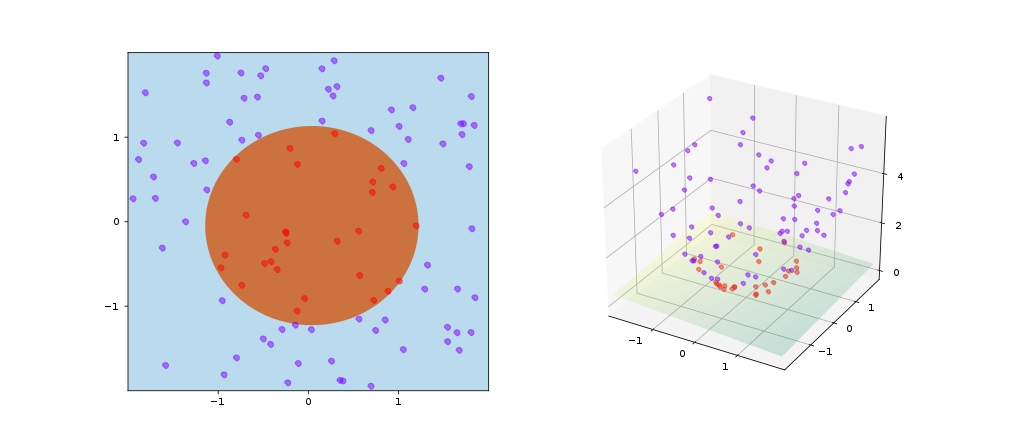
\includegraphics[width=1\textwidth]{045}
    \caption{A training example of SVM with kernel given by \(\phi((a,b)) = (a,b,a^2+b^2)\)}
\end{figure}
If every datapoint is mapped into high-dimensional space via some transformation \(\Phi: \vec{x} \to \phi(\vec{x})\), the inner product becomes
\begin{equation}
    K(\vec{x}_i,\vec{x}_j) = \phi(\vec{x}_i)^T \phi(\vec{x}_j)
\end{equation}
A kernel function is a function that is equivalent to an inner product in some feature space. It \textbf{implicitly} maps data to a high-dimensional space (without the need to compute each \(\phi(\vec{x})\) explicitly).

For some function \(K(\vec{x}_i,\vec{x}_j)\) checking that \(K(\vec{x}_i,\vec{x}_j) = \phi(\vec{x}_i)^T \phi(\vec{x}_j)\) can be cumbersome.

\subsubsection{Mercer's theorem}
Every positive semidefinite symmetric\footnote{A symmetric matrix is \textbf{positive semidefinite} if and only if all eigenales are non-negative} function is a kernel. A positive semidefinite symmetric function correspond to a positive semidefinite symmetric Gram matrix

\begin{equation}
    K = 
    \begin{bmatrix}
        K(\vec{x}_1,\vec{x}_1) & K(\vec{x}_1,\vec{x}_2) & ... & K(\vec{x}_1,\vec{x}_n) \\
        K(\vec{x}_2,\vec{x}_1) & K(\vec{x}_2,\vec{x}_2) & ... & K(\vec{x}_2,\vec{x}_n) \\
        ... & ... & ... & ... \\
        K(\vec{x}_n,\vec{x}_1) & K(\vec{x}_n,\vec{x}_2) & ... & K(\vec{x}_n,\vec{x}_n) 
    \end{bmatrix}
\end{equation}

\subsubsection{Kernels}
\begin{itemize}[topsep=0pt, partopsep=0pt]
    \item Linear: \(K(\vec{x}_i,\vec{x}_j) = \vec{x}_i^T\vec{x}_j\)\\
    \item Polynomial of power \(p\): \(K(\vec{x}_i,\vec{x}_j) = (1 + \vec{x}_i^T \vec{x}_j)^p\)\\
    \item Gaussian (radial-basis function): \(K(\vec{x}_i,\vec{x}_j) = e^{\frac {||\vec{x}_i - \vec{x}_j||^2} {2 \sigma^2}}\)\\
        \begin{itemize}
        \item Mapping \(\Phi: \vec{x} \to \phi(\vec{x})\), where \(\phi(\vec{x})\) is infinite-dimensional: every point is mapped to a function (Gaussian); combination of functions for support vectors is the separator.\\
        \end{itemize}
\end{itemize}
Higher-dimensional space still has \emph{intrinsic} dimensionality \(d\) (the mapping is \emph{onto}), but linear separators in it correspond to non-linear separators in original space.

With the kernels, the dual problem formulation becomes
\begin{align*}
    &\max_\alpha \sum_i \alpha_i - \frac 1 2 \sum_i \sum_j \alpha_i \alpha_j y_i y_j K(\vec{x}_i, \vec{x}_j)\\
    \text{s.t. } &\sum_i \sum_j \alpha_i y_i = 0, \quad \alpha_i \geq 0, \quad \forall i
\end{align*}
And finally the solution is
\begin{equation}
    f(\vec{x}) = \sum_i \alpha_i y_i K(\vec{x}_i; \vec{x}) + b
\end{equation}
The optimization techniques for finding \(\alpha_i\)'s remains the same.

\newpage
\begin{exercise}[topsep=20pt, itemsep=10pt]
    \ex[!] Describe the Support Vector Machine.
    \ex What are large margin classifiers?
    \ex What is a support vector?
    \ex How do we maximize the margin?
    \ex[!] What is the Support Vector Machine Problem?
    \ex Describe the soft margin classification.
    \ex What are the slack variables? What are they used for?
    \ex[!] Why do we need the slack variables?
    \ex What if we have non linearly separable data?
    \ex Why do we need the dual problem?
    \ex Describe the kernel trick for Support Vector Machine.
    \ex Explain the Mercer's theorem.
    \ex What is a kernel?
    \ex How does the dual problem formulation become with kernels?
    \ex[!] Does SVM use regularization? What regularizer does SVM use?
    \ex[!] Compare SVM with \(k\)-NN.
\end{exercise}

% \chapter{Ranking}
\textbf{Ranking} is the application of machine learning, typically supervised or reinforcement learning, in the construction of ranking models for information retrieval systems. Training data consists of lists of items with some partial order speicified between items in each list. This order is typically induced by giving a numerical or ordinal score or a binary judgement for each item. 

The ranking model purposes to rank, i.e. producing a permutation of items in new, unseen lists in a similar way to rankings in the training data.

\begin{figure}[h]
    \centering
    \includegraphics[width=.75\textwidth]{046}
    \caption{Ranking problems general schema.}
\end{figure}

Traditional machine learning solves a prediction problem on a single instance at a time. The aim of traiditional machine learning is to come up with a class or a single numerical score for that instance. Instead, ranking solves a ranking problem on a list of items. The aim of ranking is to come up with optimal ordering of those items. Ranking doesn't care much about the exact score that each item gets, but cares more about the relative ordering among the items.

\section{Multilabel classification}
In machine learning, \textbf{multilabel classification} and the strongly related problem of \textbf{multi-output classification} are varients of the classification problem where multiple labels may be assigned to each instance. Multilabel classification is a generalization of multiclass classification, which is the single-label problem of categorizing instances into precisely one of more than two classes; in the multi-label problem there is no constraint on how many of the classes the instance can be assigned to.

In multiclass classification each example has one label and exactly one label. In multilabel classification each example has \textbf{zero or more labels}.

Formally, multilabel classification is the problem of finding a model that maps inputs \(\vec{x}\) to binary vectors \(\vec{y}\) (assigning a value of 0 or 1 for each element - label - in \(\vec{y}\)).

Multilabel applications examples are:
\begin{itemize}[topsep={0pt}, partopsep={0pt}]
    \item Video surveillance - reidentification;
    \item Scene analysis - visual localization;
    \item Image annotation;
    \item Document topics;
    \item Medical diagnosis.
\end{itemize}

\section{Ranking problems}
Suppose we start a new web search company. Like other search engines, a userinputs a query and a set of documents is retrieved. Our goal is to rank the resulting documents based on relevance to the query. The ranking problem is to take a collection of items and sort them according to some notion of preference. One of the trickiest parts of doing ranking through learning is to properly define the loss function.

\subsection{Black box approach}
We can implement the algorithm for the preference function with the perceptron by creating the vector of the features of the two examples.

Given a generic binary classifier, we can use it to solve our new problem.
\begin{figure}[t!]
    \centering
    \includegraphics[width=1\textwidth]{047}
    \caption{Black box approach to ranking.}
\end{figure}
We need to train a classifier to decide if the first input is better than the second: we have to consider all the possible pairings of the examples in a ranking and label them as positive if the first example is higher ranked, otherwise we rank them as negative.

The problem here is that our binary classifier takes only one example as input. How can we perform the following classification?
\begin{equation}
    a_1, a_2, ..., a_n; b_1, b_2, ..., b_n \to f_1', f_2', ... f_n'
\end{equation}
We need features that compare the two examples \(a_i\) and \(b_i\), this new vector is called \textbf{combined feature vector}. There are many approaches that depend on domain and on the classifier, two common approaches to do this are:
\begin{itemize}
    \item compare by difference:
    \begin{equation*}
        f'_i = a_i - b_i
    \end{equation*}
    \item compare the first to the second example:
    \begin{equation*}
        f'_i = \begin{cases}
            1 &\text{ if } a_i > b_i\\
            0 &\text{ otherwise}\\
        \end{cases}
    \end{equation*}
\end{itemize}

\subsection{Preference function}
For each query, we are also given a collection of documents, together with a desired ranking over those documents. We'll assume that we have \(N\)-many queries and for each query we have \(M\)-many documents. The goal is to train a binary classifier to predict a \textbf{preference function}. Given a query \(q\) and two documents \(d_i\) and \(d_j\), the classifier should predict whether \(d_i\) should be preferred to \(d_j\) with respect to the query \(q\).

\subsection{Bipartite Ranking}
Bipartite ranking algorithms are useful for bipartite ranking problems. A \textbf{Bipartite ranking problem} is one in which you are trying to predict a binary response, for instance "is this document relevant or not?".

The only goal is to ensure that all the relevant documents are ahead of all the irrelevant documents. There is no notion that one relevant document is more relevan than another.

For non-bipartite ranking problems, more sophisticated methods can be used.

\begin{figure}[t!]
    \centering
    \includegraphics[width=0.75\textwidth]{099}
    \caption{Bipartite ranking example}
\end{figure}

\section{Algorithm}
A naive solution for the training algorithm of the ranking is pretty simple. As we sayed, the goal is to predict a preference function that, given a query and two documents, the clasifier should predict whether the first should be preferred to the second with respect to the query. In the following algorithm, we will assume \(N\)-many queries and for each quary we have \(M\)-many documents. 

For every \(n\) and every pair \(i \neq j\), we wil create a binary classification example based on features \(\vec{x}_{nij}\) (that denotes the features associated with comparing document \(i\) to document \(j\) on query \(n\)). This example is positive if \(i\) is preferred to \(j\), otherwise it is negative.

\begin{algorithm}
    \caption{NaiveRankTrain(RankingData, BinaryTrain)}
    \label{alg:naive_rank_train}
$D \gets [\ ]$\;
\For{$n \gets 1$ to $N$}{
    \For{$i,j \gets 1$ to $M$ and $i \neq j$}{
     \eIf{$i$ is preferred to $j$ on query $n$}{
            $D \gets D.append(\vec{x}_{nij},+1)$\;
        }{
            \If{$j$ is preferred to $i$ on query $n$}{
                $D \gets D.append(\vec{x}_{nij},-1)$\;
            }
        }
    }
}
\Return{BinaryTrain($D$)}
\end{algorithm}

We can describe a naive solution for the test phase as well. In this case we initialize a list of scorest to 0, than for each document \(d_i\) and \(d_i\) (\(i \neq j\)), we compute the score with our preference function; then we add the score to \(d_i\) and subtract the score to \(d_j\). At the end we return the queries sorted by the computed scores.

\begin{algorithm}
    \caption{NaiveRankTest($f$, $\hat{x}$)}
    \label{alg:naive_rank_test}
$score \gets \langle 0, 0, ..., 0 \rangle$\;
\For{$i,j \gets 1$ to $M$ and $i \neq j$}{
    $y \gets f(\hat{x}_{ij})$\;
    $score_i \gets score_i + y$\;
    $score_j \gets score_j - y$\;
}
\Return{$score$.sort()}
\end{algorithm}

The problem with this approach is that it's impossible to tell --- just by looking at its output on one \(i,j\) pair --- how good the overall ranking is. This is because there is the intermediate step of turning these pariwise predictions into a coherent ranking.

These algorithms actually work quite well in the case of bipartite ranking problems. This is essentially beause the only goal in bipartite ranking problems is to ensure that all the relevant documents are ahead of all the irrelevant documents. 

\section{Weighted binary classification}
For non-bipartite ranking problems, we can do better. First, when the preferences thath we get at training time are more nuanced than "relevant or not", we can incorporate these preferences at training time. Effectively, we want to give a higher weight to binary problems that are very different in terms of preference than others. Second, rather than producing a list of scores and then calling an arbitrary sorting algorithm, we can actually use the preference function as the sorting function inside our own implementation of quicksort.

Define a ranking as a function \(\sigma\) that maps the objects we are ranking to the desired position in the list \(1,2,...,M\). If \(\sigma_u < \sigma_v\) then \(u\) is preferred to \(v\). Given data with observed rankings \(\sigma\), our goal is to learn to predict rankings for new objects, \(\hat{\sigma}\). We define \(\Sigma_M\) as the set of all ranking functions over \(M\) objects. We also wish to express the fact that making a mistake on some pairs is worse than making a mistake on others - this will be encoded in a cost function \(\omega\), where \(\omega(i,j)\) is the cost for accidentally putting something in position \(j\) when it should have gone in position \(i\). To be a valid cost function, \(\omega\) should be \emph{symmetric}, \emph{monotonic}: if \(i < j < k\) then \(\omega(i,j) \leq \omega(i,k)\), \emph{satisfy the triangle inequality}: \(\omega(i,j) + \omega(j,k) \geq \omega(i,k)\).

\subsection{\(\omega\)-Ranking}
Given an input space \(\mathcal{X}\), an unknown distribution \(\mathcal{D}\) over \(\mathcal{X} \times \Sigma_M\), and a training set \(D\) sampled from \(\mathcal{D}\).\\
We want to compute a function \(f : \mathcal{X} \to \Sigma_M\) minimizing:
\begin{equation}
    \mathbb{E}_{(\vec{x},\sigma) \sim \mathcal{D}} \left[ \sum_{u \neq v} [\sigma_u < \sigma_v][\hat{\sigma}_v < \hat{\sigma}_u] \omega ( \sigma_u , \sigma_v ) \right]
\end{equation}
where \(\hat{\sigma} = f(\vec{x})\).

In this definition, the only complex aspect is the loss function. This loss sums over all pairs of objects \(u\) and \(v\), but the predicted ranking \(\hat{\sigma}\) prefers \(v\) to \(u\), then you incur a cost of \(\omega(\sigma_u,\sigma_v)\).

Depending on the problem you care about, you can set \(\omega\) to many "standard" options. If \(\omega(i,j) = 1\) whenever \(i \neq j\), then you achieve the Kemeny distance measure, which simly counts the number of airwise misordered items. We may only care about getting the top \(K\) predictions correct. In this case, we define:
\begin{equation}
    \omega(i,j) = \begin{cases}
        1 &\text{if min}\{i,j\} \leq K \text{ and } i \neq j\\
        0 &\text{otherwise}\\
    \end{cases}
\end{equation}
In this case, only errors in the top \(K\) elements are penalized. Swapping items 55 and 56 is irrelevent (for \(K < 55\)).

\begin{algorithm}
    \caption{RankTrain($D^\text{rank}$, $\omega$, BinaryTrain)}
    \label{alg:rank_train}
$D^\text{bin} \gets [\ ]$\;
\For{$(\vec{x},\sigma) \in D^\text{rank}$}{
    \For{$u \neq v$}{
        $y \gets \text{sign}(\sigma_v - \sigma_u))$\;
        $w \gets \omega(\sigma_u - \sigma_v)$\;
        $D^\text{bin} \gets D^\text{bin} \oplus (y,w,\vec{x}_{uv})$\;
    }
}
\Return{BinaryTrain($D^\text{bin}$)}
\end{algorithm}

At test time, instead of predicting scores and then sorting hte list, as in the previous algorithm, we run the quicksort algorithm, using the learned function as a comparison function. In practice at teach step a pivot \(p\) is chosen. Every object \(u\) is compared to \(p\) using the learned function and sorted to left or right. The difference between this algorithm and quicksort is that the comparison function is \emph{probabilistic}. If \(f\) outputs probabilities, for instance it predicts that \(u\) has an 80\% probability of being better than \(p\), then it puts it on the left with 80\% probability and on the right with 20\% probability.

\begin{algorithm}
    \caption{RankTest($f$, $\hat{x}$, $obj$)}
    \label{alg:rank_test}
\eIf{$obj$ contains 0 or 1 elements}{
    \Return{$obj$}
}{
    $p \gets$ randomly chosen object in $obj$\;
    $left \gets [\ ]$\;
    $right \gets [\ ]$\;
    \For{$u \in obj \setminus \{p\}$}{
        $\hat{y} \gets f(\vec{x}_{up})$\;
        \eIf{uniform random variable < $\hat{y}$}{
            $left \gets left \oplus u$\;
        }{
            $right \gets right \oplus u$\;
        }
    }
    $left \gets $ RankTest($f, \hat{x}, left$)\;
    $right \gets $ RankTest($f, \hat{x}, right$)\;
}
\Return{$left \oplus \langle p \rangle \oplus right$}
\end{algorithm}
This algorithm is better than the naive algorithm in at least two ways. First, it only makes \(O(M \log_2 M)\) calls to \(f\) rather than \(O(M^2)\) calls in the naive case. Second, it achieves a better error bound.

\newpage\null
\newpage
\begin{exercise}[topsep=20pt,itemsep=10pt]
    \ex[!] Describe the ranking.
    \ex What is multilabel classification? Give some application example.
    \ex[!] Can I use the perceptron to do ranking?
    \ex What is the preference function?
    \ex Describe the bipartite ranking problem.
    \ex[!] How can the binary classifier problem be solved?
    \ex Describe the weighted binary classification.
    \ex Provide and describe the weighted ranking training algorithm.
    \ex Provide and describe the weighted ranking testing algorithm.
\end{exercise}

% \chapter{Neural Networks}
Artificial neural networks are computing systems inspired by the biological neural networks that constitute animal brains. An ANN is based on a collection of connected units or nodes called \textbf{artificial neurons}, which loosely model the neurons in a biological brain. Each connection, like the synapses in a biological brain, can transmit a signal to other neurons. An artificial neuron receives a signal then processes it and can signal neurons connected to it. The signal at a connection is a real number, and the output of each neuron is computed by some non-linear function of the sum of its inputs. The connections are called \textbf{edges}. Neurons and edges typically have a \textbf{weight} that adjusts as learning proceeds. The weight increases or decreases the strength of the signal at a connection. Neurons may have a threshold such that a signal is sent only if the aggregate signal crosses that threshold. Typically, neurons are aggregated into layers. Different layers may perform different transformations on their inputs. Signals travel from the first layer, to the last layer, possibly after traversing the layers multiple times.

\begin{wrapfigure}{l}{0.35\textwidth}
    \begin{center}
        \includegraphics[width=0.25\textwidth]{053}
        \caption{An artificial neural network as an interconnected group of nodes.}
    \end{center}
    \label{fig:053}
\end{wrapfigure}

The idea of neural networks began unsurprisingly as a model of how neurons in the brain function, termed 'connectionism' and used connected circuits to simulate intelligent behaviour .In 1943, portrayed with a simple electrical circuit by neurophysiologist Warren McCulloch and mathematician Walter Pitts. Donald Hebb took the idea further in his book, The Organization of Behaviour (1949), proposing that neural pathways strengthen over each successive use, especially between neurons that tend to fire at the same time thus beginning the long journey towards quantifying the complex processes of the brain.

Around this time, Frank Rosenblatt, a psychologist at Cornell, was working on understanding the comparatively simpler decision systems present in the eye of a fly, which underlie and determine its flee response. In an attempt to understand and quantify this process, he proposed the idea of a Perceptron in 1958, calling it \textbf{Mark I Perceptron}. It was a system with a simple input output relationship, modeled on a McCulloch-Pitts neuron, proposed in 1943 by Warren S. McCulloch, a neuroscientist, and Walter Pitts, a logician to explain the complex decision processes in a brain using a linear threshold gate. A McCulloch-Pitts neuron takes in inputs, takes a weighted sum and returns '0' if the result is below threshold and '1' otherwise.

\begin{figure}[h]
    \centering
    \includegraphics[width=.75\textwidth]{048}
    \caption{A McCulloch-Pitts neuron.}
\end{figure}

A major drawback? This perceptron could only learn to separate linearly separable classes, making the simple but non-linear exclusive-or circuit an insurmountable barrier.

\section{From Perceptron to Deep Networks}
In 1969 it was formally proved that perceptron cannot be used for non-linearly separable problems. In particular, it has been proved that the \textbf{XOR} (exclusive or) cannot be solved with the perceptron. We can realize the XOR as a function that map all pairs of input \(x_1\) and \(x_2\) to an output \(y\) with the following scheme:
\begin{table}[h!]
\begin{center}
\begin{tabular}{|p{0.8cm}|p{1.2cm}|p{1.2cm}|}
    \hline
    \(x_1\) & \(x_2\) & \(y\) \\
    \hline
    1 & 1 & 0 \\
    \hline
    1 & 0 & 1 \\
    \hline
    0 & 1 & 1 \\
    \hline
    0 & 0 & 0 \\
    \hline
\end{tabular}
\end{center}
\caption{XOR truth table}
\end{table} 

Despite the messy and somewhat dis-satisfactory advent of the use of Machine Learning to quantify decision systems apart from the brain, today's artificial neural networks are nothing more than \textbf{several layers of these perceptrons}.

\subsubsection{Multi-Layer Perceptron}
The idea of the multi-layer perceptron is to densely connect artifical neurons to realize compositions of non-linear functions. THe information is propagated from the inputs to the outputs. No cycles between outputs and inputs (DAG). Compute one or more non-linear function. Computation is carried out by composition of some number of algebraic functions implemented by the connections, weights and biases of the hidden and output layers. Hidden layers compute intermediate representations.

One of the problems that arose was with the impractically long runtimes required for running these networks given that this was the 60s apart from its inability to learn simple boolean exclusive-or circuits.

Multi-layer networks use a variety of learning techniques, the most popular being backpropagation. Here, the output values are compared with the correct answer to compute the value of some predefined error-function. By various techniques, the error is then fed back through the network. Using this information, the algorithm adjusts the weights of each connection in order to reduce the value of the error function by some small amount. After repeating this process for a sufficiently large number of training cycles, the network will usually converge to some state where the error of the calculations is small. In this case, one would say that the network has learned a certain target function.

\subsection{Backpropagation}
\textbf{Backpropagation}, a method devised by researchers since the 60's and continuously developed on well into the AI winter, was an intuition based method that attributed reducing significance to each event as one went farther back in the chain of events. Backpropagation along with Gradient Descent forms the backbone and powerhouse of neural networks. While Gradient Descent constantly updates and moves the weights and bias towards the minimum of the cost function, backpropagation evaluates the gradient of the cost w.r.t. weights and biases, the magnitude and direction of which is used by gradient descent to evaluate the size and direction of the corrections to weights and bias parameters.

\begin{figure}[h!]
    \centering
    \includegraphics[width=.5\textwidth]{050}
    \caption{Backpropagation scheme.}
\end{figure}

\subsubsection{In a nutshell}
\begin{enumerate}
    \item Forward propagation: sum inputs, produce activations, feed-forward.
    \item Error estimation.
    \item Back propagate the error signal and use it to update weights.
\end{enumerate}
The main idea is that given training samples \(T = \{(x_1, y_1), (x_2, y_2), ..., (x_n, y_n)\}\), adjust the weights of the network \(\Theta\) such that a cost function is minimized
\begin{equation}
    \min_{\Theta} \sum_i L(y_i, f(x_i; \Theta))
\end{equation}
Choose the loss function (e.g. L2), update the weights of each layer with gradient descend, and use backpropagation of the error signal to compute the gradient efficiently.

\section{Feedforward Networks}
A feedforward neural network is an artificial netowkr wherein connections between the nodes do not form a cycle. The feedforward neural network was the first and simplest type of artificial neural network devised. In this network, the information moves in only one direction --- forward --- from the input nodes, through the hidden nodes (if any) and to the output nodes.

Feedforward neural networks are the quintessential deep learning models. The goal of a feedforward network is to approximate some function \(f^*: \mathcal{X} \to \mathcal{Y}\). For example, for a classifier, \(y = f^*(\vec{x})\) maps an input \(\vec{x}\) to a category \(y\). A feedforward network defines a mapping \(\vec{y} = f(\vec{x}; \vec{\Theta})\) and learns the value of the parameters \(\vec{\Theta}\) that result in the best function approximation.

Feedforward neural networks are called \textbf{networks} because they are typically represented by composing together many different functions. The model is associated with a directed acyclic graph describing how the functions are composed together. For example, we might have three functions \(f^{(1)}\), \(f^{(2)}\), and \(f^{(3)}\) connected in a chain, to form \(f(\vec{x}) = f^{(3)}(f^{(2)}(f^{(1)}(\vec{x})))\). 

\begin{figure}[h]
    \centering
    \includegraphics[width=.75\textwidth]{049}
    \caption{The function \(f\) is a composition of multiple functions.}
\end{figure}

These chain structures are the most commonly used structures of neural networks. In this case, \(f^{(1)}\) is called \textbf{first layer} of the network, \(f^{(2)}\) is the \textbf{second layer} of the network, and so on. The overall length of the chain gives the \textbf{depth} of the model. The final layer is the \textbf{output layer} of the model.

\subsection{Training}
During the training, we drive \(f(\vec{x}; \Theta)\) to match \(f^*(\vec{x})\). The training data provides us with noisy, approximate examples of \(f^*(\vec{x})\) evaluated at different training points.

The training examples specify directly what the output layer must do at each point \(\vec{x}\); it must produce a value that is close to \(y\). The behavior of the other layers is not directly specified by the training data. The learning algorithm must decide how to use those layers to produce the desired output, but the training data do not say what each individual layer should do. Instead, the learning algorithms must decide how to use these layers to best implement an approximation of \(f^*\). Because the training data does not show the desired output for each of these layers, they are called \textbf{hidden layers}.

Designing and training a neural network is not much different from training any other machine learning model with gradient descent. The largest difference between the linear models we have seen so far and neural networks is that the nonlinearity of a neural network causes most interesting loss functions to become non-convex. This means that neural networks are usually trained by using iterative, gradient-based optimizers that merely drive the cost function to a very low value, rather than the linear equation solvers used to train linear regression models or the convex optimization algorithms with global convergence guarantees used to train logistic regression or SVMs. Convex optimization converges starting from any initial parameters.

\begin{figure}[t!]
    \centering
    \includegraphics[width=.75\textwidth]{054}
    \caption{Ball diagram depicting the visualization of how gradient based learning occur.}
\end{figure}

In order to apply gradient descent to train our neural network, we need to specify our model, that means that we need to specify the input and output layers are made, and also the cost function.

\subsubsection{Cost Function}
The cost function, for any other machine learning algorithm, is the loss function that measures the discrepancy between the prediction of the model given the current parameters and the ground truth labels.

It is common for neural network, when we have classification problems, to apply cost function that is called \textbf{cross-entropy loss}. It is common for neural networks to transform the outputs (scores/logits) to probability, then we can think that a good cost function can be this:
\begin{equation}
    \mathcal{L}_i = - \sum_k y_k \log(S(l_k)) = -log(S(l))
\end{equation}
That is the cross-entropy loss. The choice of the loss is related to the choice of the input unit. In this case we have decised to put a normalization operator that is the softmax loss \(S(l_i) = \frac {e^{l_i}} {\sum_k e^{l_l}}\), where \(l_i\) are the scores. Linear layer produces unnormalized log probabilities, but it is desirable to produce normalized probabilities in the output layer, that's the reason why we use the softmax.
\begin{figure}[h!]
    \centering
    \includegraphics[width=.75\textwidth]{051}
    \caption{}
\end{figure}

\subsubsection{Activation function}
The activation functions are implemented inside the \textbf{hidden units}, because here we compute affine transformation \(z = W^Tx + b\), and the non-linearity is applied that we define as \(h(z)\). There are a lot of choices for \(h\), so we have to choose it wisely.

The design of the hidden units is an active area of research. However the most popular is the \textbf{ReLU}, where \(h(x) = \max(0,x)\). Here, the gradient is 0 or 1, similar to the linear units, easy to optimize. In fact it gives 1 if the gradient unit is active.

Potential problems with the ReLU activation function are that it is non-differentiable at zero, however, it is differentiable anywhere else, and the value of the derivate at zero can be arbitrarily chose to be 0 or 1; it is not zero-centered and it is unbounded; furthermore, the bigger problem is the \textbf{dying ReLU problem}: neurons can sometimes be pushed into states in which they become inactive for essentially all inputs. In this state, no gradients flow backward through the neuron, and so the neuron becomes stuck in a perpetually inactive state and \emph{dies}. This is a form of the vanishing gradient problem. In some cases, large numbers of neurons in a network can become stuck in dead states, effectively decreasing the model capacity. This problem typically arises when the learning rate is set too high. 

In order to mitigate these problems, there are some variants,for example: the Leaky ReLU, with \(y_i = a_ix_i\); the Randomized Leaky ReLU, with \(y_{ji} = a_{ji}x_{ji}\). 

Other variation of activation function are classical squashing type of non-linearity, for example the \textbf{Sigmoid}, with \(h(x) = \frac 1 {1 + e^{-x}}\) and the \textbf{Hyperbolic tangent}, with \(h(x) = \frac {e^x - e^{-x}} {e^x + e^{-x}}\).

\subsubsection{Architecture}
How do we decide the depth and the width of a neural network? There are not many theoretical advice for that, the only relevant result is that 2-layer net with linear output with some squashing non-linearity in hidden units can approximate any continuous function over compact domain to arbitrary accuracy (given enough hidden units).

The theorem also holds for other non-linear functions. The implication of this theorem is that regardless of function we are trying to learn, we know a large MLP can represent this function.

However, we are not guaranteed that our training algorithm will be able to learn that function.

\section{Backpropagation}
Backpropagationis a widely used algorithm for training feedforward neural networks. In fitting a neural network, backpropagation computes the gradient of the loss function with respect to the weights of the network for a signle input-output example, and does so efficiently, unlike a naive direct computation of the gradient with respect to each weight individually. This efficiency makes it feasible to use gradient methods for training multilayer networks, updating weights to minimize loss; gradient descent, or variants, are commonly used. The backpropagation algorithm works by computing the gradient of the loss function with respect to each weight by the chain rule, computing the gradient one layer at a time, iterating backward from the last layer to avoid redundant calculations of intermediate terms in the chain rule; this is an example of dynamic programming.

The idea of backpropagation is a flow starting from the input layers and goes on through the hidden layers until they reach the output layer. Then the computed prediction of the network is compared with the ground truth and the error signal is computed. The error signal is backpropagated to the network in order to compute the gradient and to update all the weights associated to this connection.

There are three main steps:
\begin{enumerate}
    \item \textbf{Feedforward propagation}: accept input \(x\), pass through intermediate stages and obtain output;
    \item Use the computed output to compute a \textbf{scalar cost} depending on the loss function;
    \item \textbf{Backpropagation} allows information to flow backwards from cost to compute the gradient.
\end{enumerate}

In backpropagation we use \textbf{gradient descent}: we need error derivatives for all the weights in the net.
\begin{equation}
    w^{(1)}_{11} := w^{(1)}_{11}-\eta \frac {\delta L} {\delta w^{(1)}_{11}}
\end{equation}
From the training data we do not know what the hidden units should do, but we can compute hwo fast the error changes as we change a hidden activity.

Each hidden unit can affect many output units and have separate effeccts on error, then we combine these effects. We can compute the \textbf{error derivatives for hidden units efficiently}. Once we have error derivatives for hidden activities, it is easy to get error derivatives for weights going in.

\subsection{Step 1: Feedforward propagation}
\begin{figure}[h]
    \centering
    \includegraphics[width=.75\textwidth]{052}
    \caption{Feedforward operation.}
    \label{fig:052}
\end{figure}
In this step we go from our input to the output, with respect to Figure~\ref{fig:052}
\begin{equation}
    \hat{y} (\vec{x}; \vec{w}) = f \left( \sum_{j=1}^m w_j^{(2)} h \left( \sum_{i=1}^d w_{ij}^{(1)} x_i + w_{0j}^{(1)} \right) + w_0^{(2)} \right)
\end{equation}

\subsection{Step 2: Compute error and train}

The error of the network on a training set is
\begin{equation}
    L(X; \vec{w}) = \sum_{i=1}^N \frac 1 2 (y_i - \hat{y}(\vec{x}_i; \vec{w}))^2
\end{equation}
There is no closed-form solution. To train, we need to apply the gradient descent.

It means that we need to evaluate the derivative of \(L\) on a single example. We can consider a simple linear model for output \(\hat{y} = \sum_j w_j x{ij}\):
\begin{equation}
    \frac {\delta L(\vec{x}_i)} {\delta w_j} = (\hat{y}_i - y_i) x{ij}
\end{equation}

\subsection{Step 3: Backpropagation}
We need to compute the derivative of the error with respect to the weights, and these weights are the weights associated to the intermediate layers. The general unit activation in a multilayer network is
\begin{equation}
    z_t = h \left( \sum_j w_{jt} z_j \right)
\end{equation}

In forward propagation we calculate for each unit \(a_t = \sum_j w_{jt} z_j\). The loss \(L\) depends on \(w_{jt}\) only through \(a_t\). We are interested on computing
\begin{equation}
    \frac {\delta L} {\delta w_{jt}} = \frac{\delta L} {\delta a_t} \frac {\delta a_t} {\delta w_{jt}} = \frac {\delta L} {\delta a_t} z_j
\end{equation}
Now we are left of the problem of computing \(\frac {\delta L} {\delta a_t} z_j\). The key idea of backpropagation is that it can be computed recursively starting from the final layer to the earliest layer.

In the case of the last layer, \(\frac {\delta L} {\delta a_t} z_j\) corresponds to \(\hat{y} - y\), this is called the final error. The local error associated to the earlies layer can be computed as follows:
\begin{equation}
    \frac {\delta L} {\delta a_t} z_j = \sum_{s \in S} \frac {\delta L} {\delta a_s} \frac {\delta a_s} {\delta a_t} = h'(a_t) \sum_{s \in S} w_{ts} \frac {\delta L} {\delta a_s} z_j
\end{equation}
where \(a_s = \sum_{j:j \to s} w_{js} h(a_j)\).

\section{Training a Neural Network}
While training a Feedforward network, we need to do some modeling choices, for instance, we need to choose: the cost function, the form of output, the activation functions, the architecture (e.g. number of layers), and the \textbf{optimizer} (for the training).

Given a set of training samples \(T = \{(x_1, y_1), (x_2, y_2), ..., (x_N, y_N)\}\), the main idea of the training is to adjust all the weights of the network \(\Theta\) such that a cost function is minimized:
\begin{equation}
    \min_\Theta \sum_i L\left(y_i, f(x_i, \Theta)\right)
\end{equation}
We have to choose our loss function (e.g. L2, cross-entropy), and update the weights of each layer with gradient descent. It can be used the backpropagation of the error signal to compute the gradient efficiently.

\subsection{Gradient Descent}
Recall that the gradient is the vector of partial derivates with respect to all the coordinates of the weights:
\begin{equation}
    \nabla_wL = \left[ \frac {\delta L} {\delta w_1} \frac {\delta L} {\delta w_2} \cdots \frac {\delta L} {\delta w_N} \right]
\end{equation}
Each partial derivate measures how fast the loss changes in one direction. When the gradient is zero, i.e. all the partials derivates are zero, the loss is not changing in any direction.

Gradient descent finds the set of parameters that makes the loss as small as possible. The change of parameters depends on the gradients of the loss with respect to the network weights. Backpropagation is a method for computing gradient.

In order to define our optimization methods, let's see first the \textbf{Gradient Descent Rule}
\begin{algorithm}
    \caption{Vanilla Gradient Descent}
    \label{alg:vanilla_grad_desc}
\While{True}{
    $weights\_grad \gets $ evaluate\_gradient($loss\_fun$, $data$, $weights$)\;
    $weights \gets weights + step\_size \cdot weigths\_grad$\;
}
\end{algorithm}

\subsubsection{Batch Gradient Descent}
In BGD, all the training data is taken into consideration to take a single step. We take the average of the gradients of all the training example and then use that mean gradient to update our parameters. So that's just one step of gradient descent in one epoch.

\begin{algorithm}
    \caption{BatchGradientDescent($k$)}
    \label{alg:batch_gradient_descent}
\KwData{Learning rate $\epsilon_k$}
\KwData{Initial parameter $\Theta$}
    \While{stopping criteria is not met}{
        Compute gradient estimate over $N$ examples:\\
        $\hat{g} \gets \frac 1 N \nabla_\Theta \sum_i L\left( f(\vec{x}^{(i)}; \Theta), \vec{y}^{(i)} \right)$\;
        Apply Update: $\Theta \gets \Theta - \epsilon \hat{g}$\;
    }
\end{algorithm}

A pro of this algorithms is that the gradient estimates are stable, on the other hand it need to compute gradients over the entire training for one update.

\subsubsection{Stochastic Gradient Descent}
To tackle this problem we have Stochastic Gradient Descent. In Stochastic Gradient Descent (SGD), we consider just one example at a time to take a single step.

\begin{algorithm}
    \caption{StochasticGradientDescent($k$)}
    \label{alg:stochastic_gradient_descent}
\KwData{Learning rate $\epsilon_k$}
\KwData{Initial parameter $\Theta$}

    \While{stopping criteria is not met}{
        Sample example $(\vec{x}^{(i)}, \vec{y}^{(i)})$ from training set\;
        Compute gradient estimate:\\
        $\hat{g} \gets \nabla_\Theta L\left( f(\vec{x}^{(i)}; \Theta), \vec{y}^{(i)} \right)$\;
        Apply Update: $\Theta \gets \Theta - \epsilon \hat{g}$\;
    }
    
\end{algorithm}

A problem with this algorithm is that gradient estimates can be very noisy. One possible solution can be to use larger \textbf{mini-batches}. The advantage is that the computation time per update does not depend on the number of training examples \(N\), so it permits computation on extremely large datasets. This solution is often done with a parallel implemenetation. Using GPUs it is common for power of 2 batch sizes to offer better runtime (some kinds of hardware achieve better runtime with specific sizes of arrays).

\subsubsection{Momentum}
The progress to the minimum with SGD is very slow along a flat direction, it causes jitter along the steep one.

So we can use the SDG with \textbf{momentum}, that introduces a new variable \(\vec{v}\), the velocity. The velocity is an exponentially decaying moving average of the negative gradient.

\begin{algorithm}
    \caption{StochasticGradientDescent with Momentum}
    \label{alg:stochastic_gradient_descent_momentum}
\KwData{Learning rate $\epsilon_k$}
\KwData{Momentum parameter $\alpha$}
\KwData{Initial parameter $\Theta$}
\KwData{Learning velocity $\vec{v}$}

    \While{stopping criteria is not met}{
        Sample example $(\vec{x}^{(i)}, \vec{y}^{(i)})$ from training set\;
        Compute gradient estimate:\\
        $\hat{g} \gets \nabla_\Theta L\left( f(\vec{x}^{(i)}; \Theta), \vec{y}^{(i)} \right)$\;
        Compute the velocity update:\\
        $\vec{v} \gets \alpha \vec{v} - \epsilon \hat{g}$\;
        Apply Update: $\Theta \gets \Theta - \vec v$;
    }
    
\end{algorithm}

\subsubsection{Adaptive Learning Rate Methods}
So far we have assigned the same learning rate to all features. If the features vary in importance and frequency, is this a good idea? The learning rate is one of the hyperparameters most difficult to set.

\section{Convolutional Neural Networks}
\textbf{Convolutional Neural Network} (CNN or ConvNet) is a class of artificial neural network, most commonly applied to analyze visual imagery.  Neural networks are extremely powerful in applications that deal with an input space which is locally structured, i.e. spatial or temporal, for example images and language, and that deal with an arbitrary input of features.

The name "convolutional neural network" indicates that the network employs a mathematical operation called convolution. Convolutional networks are a specialized type of neural networks that use convolution in place of general matrix multiplication in at least one of their layers.

A convolutional neural network consists of an input layer, hidden layers and an output layer. In any feed-forward neural network, any middle layers are called hidden because their inputs and outputs are masked by the activation function and final convolution. In a convolutional neural network, the hidden layers include layers that perform convolutions.

\subsection{Convolutional layers}
In a CNN, the input is a tensor with a shape: given the number of inputs \(n\), the input height \(h\), the input width \(w\), and the input channels \(c\), the shape \(s\) is defined as:
\begin{equation}
    s = n \cdot h \cdot w \cdot c
\end{equation}
After passing through a conolutional layer, the image becomes abstracted to a feature map, also called an activation map.

Convolutional layers convolve the input and pass its result to the next layer. This is similar to the response of a neuron in the visual cortex to a specific stimulus. Each convolutional neuron processes data only for its receptive field. Although fully connected feedforward neural network can be used to learn features and classify data, this architecture is generally impractical for larger inputs such as high resolution images. It would require a very high number of neurons, even in a shallow architecture, due to the large input size of images, where each pixel is a relevant input feature. For instance, a fully connected layer for a (small) image of size 100 x 100 has 10,000 weights for each neuron in the second layer. Instead, convolution reduces the number of free parameters, allowing the network to be deeper. For example, regardless of image size, using a 5 x 5 tiling region, each with the same shared weights, requires only 25 learnable parameters. Using regularized weights over fewer parameters avoids the vanishing gradients and exploding gradients problems seen during backpropagation in traditional neural networks.

In practice, CNN learns a hierarchy of features. Each layer of hierarchy extracts features from the output of the previous layer, and then trains all layers jointly.

Furthermore, convolutional neural networks are ideal for data with a grid-like topology (such as images) as spatial relations between separate features are taken into account during convolution and/or pooling.

\begin{figure}[h!]
    \centering
    \includegraphics[width=.75\textwidth]{055}
    \caption{}
    \label{fig:055}
\end{figure}

Convolutional neural networks are Feedforward neural networks with a specialized connectivity structure, where multiple layers of feature extractors are stacked: low-level layers extract local features, and high-level layers learn global patterns. Typically CNN layers transform the input matrix into an output class prediction. There are a few distinct types of operations:
\begin{itemize}[topsep={0pt}, partopsep={0pt}]
    \itemsep0pt
    \item Convolution
    \item Non-linearity
    \item Pooling
\end{itemize}

\subsubsection{Convolution}
\begin{wrapfigure}{l}{0.35\textwidth}
    \begin{center}
        \includegraphics[width=0.25\textwidth]{056}
        \caption{}
    \end{center}
    \label{fig:056}
\end{wrapfigure}

The convolution is a mathematical operation on two functions \(f\) and \(g\) that produces a third function \(f \cdot g\) that expresses how the shape of one is modified by the other. It is a general purpose filter operation for images. A kernel matrix is applied to an image, and it works by determining the value of a central pixel by adding the weighted values of all its neighbors together. The output is a new modified (filtered) image, and it can be used to smooth, sharpen, enhance, etc.
\begin{equation}
    S(i,j) = (I \cdot K)(i,j) = \sum_m \sum_n I(m,n)K(i-m,j-n)
\end{equation}

The convolution layer is the core layer of the CNN, it consists of a set of filters, and each filter covers a spatially small portion of the input data (receptive field) and is convolved across the dimensions of the input data, producing a multi-dimensional feature map.

\begin{wrapfigure}{r}{0.35\textwidth}
    \begin{center}
        \includegraphics[width=0.25\textwidth]{058}
        \caption{}
    \end{center}
    \label{fig:058}
\end{wrapfigure}

The intuition is that the network will learn filters that activate when they see some specific type of feature at some spatial position in the input.

The filter is smaller than the input data and the type of multiplication applied between a filter-sized patch of the input and the filter is a dot product. A dot product is the element-wise multiplication between the filter-sized patch of the input and filter, which is then summed, always resulting in a single value. Because it results in a single value, the operation is often referred to as the “scalar product“.

Using a filter smaller than the input is intentional as it allows the same filter (set of weights) to be multiplied by the input array multiple times at different points on the input. Specifically, the filter is applied systematically to each overlapping part or filter-sized patch of the input data, left to right, top to bottom.

\begin{figure}[h!]
    \centering
    \includegraphics[width=.5\textwidth]{057}
    \caption{An example of an input data with a filter and the output of the total convolution.}
    \label{fig:057}
\end{figure}

\subsubsection{Non-linearity}
After the convolution, the non-linearity is computed. The result of the convolution as in the feedforward neural network is then passwd to an activation function (e.g. ReLO or Sigmoid)
\begin{align*}
    y_{i,j} = &f(a_{i,j})\\
    \text{e.g. } &f(a) = \left[a\right]_+\\
    &f(a) = sigmoid(a)
\end{align*} 
We are using non-linearity in order to have a final non-linear representation for our prediction model and, more importantly, since the non-linearity is applied element-wise, it does not affect the receptive field of the neural network.

\subsubsection{Spatial Pooling}
After the application of the non-linearity, there is a downsampling operation, called \textbf{spatial pooling}, and it is used to provide invariance to small traslation of the input.

There are several non-linear functions to implement pooling, where max pooling is the most common. It partitions the input image into a set of rectangles and, for each such sub-region, outputs the maximum. 

Intuitively, the exact location of a feature is less important than its rough location relative to other features. This is the idea behind the use of pooling in convolutional neural networks. The pooling layer serves to progressively reduce the spatial size of the representation, to reduce the number of parameters, memory footprint and amount of computation in the network, and hence to also control overfitting. This is known as down-sampling. It is common to periodically insert a pooling layer between successive convolutional layers (each one typically followed by an activation function, such as a ReLU layer) in a CNN architecture.
\begin{equation}
    x_{i,j} = \max_{|k| < \tau , |l| < \tau} y_{i-k,j-l}
\end{equation}

\begin{figure}[h!]
    \centering
    \includegraphics[width=.75\textwidth]{059}
    \caption{Example of max pooling.}
    \label{fig:059}
\end{figure}

\section{Other Neural Networks}
\begin{figure}[t!]
    \centering
    \includegraphics[width=.75\textwidth]{060}
    \caption{Many models for different needs.}
    \label{fig:060}
\end{figure}

In particular so far we have discussed the Perceptron, the Feedforward neural network, and the Deep Feedforward neural network, where we have multiple hidden layers.

So far, we focused mainly on prediction problems with fixed-size inputs and outputs. We discussed the flexibility of CNN to address a wide range of task, but what if the input and/or output is a variable-length sequence? There are many applications where we need this, for example document classification, sentiment analysis, or image captioning.

\subsection{Recurrent Neural Networks}
For this problem, different type of neural networks are required. Let's consider an example, a video frame prediction, given a video, the model should predict the category of each frame of the video --- this example could be useful for segmenting a movie in different parts. Until now, we have seen a \textbf{Single2Single} type of neural network, the feedforward neural network, where we have given a single object as input and we want to predict a single object as output. But for this problem we need to implement a \textbf{Multiple2Multiple} network, the \textbf{Recurrent Network}, that has been designed in problems in which we have multiple object as input and we want to predict multiple objects as output. Note that there is another type of neural network, the \textbf{Single2Multiple}, where I have for example a single image and I want to predict multiple captions of the image.

For the problems above, Feedforward neural networks and Convolutional neural networks cannot be applied. The choice in this case is to apply another type of neural network, where, given an input \(x_t\), the neural network passes the input to an input layer that learns an hidden representation \(h_t\) that could be eventually used by a classifier to perform some output prediction \(y_t\).

Notice that the particularity of the Recurrent Neural Network is the \textbf{recurrence formula}, that is a function of certain parameters of the network that relates the input at time \(t\) and the latent representation of the previous state with the latent representation of the current state:
\begin{equation}
    h_t = f_W(x_t, h_{t-1})
\end{equation}
These recurrents operations take into account the concept of time/sequence processing, and can be better understood by unrolling the formula with the scheme in Figure~\ref{fig:061}. 
\begin{figure}[h!]
    \centering
    \includegraphics[width=.75\textwidth]{061}
    \caption{Recurrent neural network.}
    \label{fig:061}
\end{figure}

\subsection{Autoencoders}
\textbf{Autoencoders (AE)} are somwhat similar to FFNNs as AEs are more like a different use of FFNNs than a fundamentally different architecture. The basic idea behind autoencoders is to encode information (as in compress, not encrypt) automatically, hence the name. The entire network always resembles an hourglass like shape, with smaller hidden layers than the input and output layers. AEs are also always symmetrica around the middle layer(s). The smalles layers are almost always in the middle, the place where the information is most compressed. Everything up to the middle is called the encoding part, everything after the middle the deconding and the middle is called the code. One can train them using backpropagation by feeding input and setting the error to be the difference between the input and what came out. AEs can be built symmetrically when it comes to weights as well, so the encoding weights are the same as the decoding weights.

Autoencoders can be considered as an unsupervised approach for learning a lower-dimensional feature representtion from unlabeled data.

\begin{figure}[h!]
    \centering
    \includegraphics[width=.5\textwidth]{062}
    \caption{Autoencoders scheme example.}
    \label{fig:062}
\end{figure}

For instance, if the input is a bunch of image, in the autoencoder there is a network --- the encoder network --- that maps the original input data into low-dimensional latent representations.

Encoders can be realized in several ways, for instance they can be realized by linear layers + nonlinearity (e.g. sigmoid), can be realized by a deep fashion by concatenating multiple fully-connected layers, or it can be realized in a convolutional fashion by having some convolutional layers and ReLU activation function one after the other.

\begin{wrapfigure}{l}{0.35\textwidth}
    \begin{center}
        \includegraphics[width=0.25\textwidth]{064}
        \caption{}
    \end{center}
    \label{fig:064}
\end{wrapfigure}

Independently of the encoder, the main idea is that the representation of the output \(z\) should be smaller than the input \(x\), so the encoder should perform dimensionality reduction. 

How to learn this feature representation? The idea is to train the autoencoder so that features can be used to reconstruct original data --- autoencoding: encoding itself.

Once we decided the architecture of the encoder and the consequent architecture of the decoder, we need a loss function, and in the case of the autoencoders the loss function is a reconstruction function that minimizes the difference between the original data and the reconstructed version of the input data:
\begin{equation}
    ||x - \hat{x}||^2
\end{equation}
\begin{figure}[h!]
    \centering
    \includegraphics[width=.5\textwidth]{063}
    \caption{Autoencoders with loss function.}
    \label{fig:063}
\end{figure}

Autoencoders are aimed to learn the latent representation \(z\), so the most common use of autoencoders is to use the common feature \(z\) in order to initialize a feature model. This means that once we have trained the autoencoder, we throw away the decoder, and we only take the latent representation \(z\) and we append the loss funcion \(\hat{y}\) and the the encoder now can be used to have a better initialization of a supervised model.

\newpage
\begin{exercise}[topsep=20pt,itemsep=10pt]
    \ex Describe a general neural network.
    \ex[!] Describe the Feedforward Neural Networks.
    \ex[!] What is backpropagation? Describe it's steps.
    \ex How do we train a neural network?
    \ex Describe the Batch Gradient Descent.
    \ex Describe the Stohastic Gradient Descent.
    \ex[!] What is the momentum? How do we update the neural network with the momentum?
    \ex Describe the momentum paramether \(\alpha\), how does it influence the momentum?
    \ex[!] Describe the Convolutional Neural Networks.
    \ex[!] Describe the Convolution layer.
    \ex[!] What is the non-linearity in the neural network? Where do we apply it?
    \ex[!] Describe the Spatial Pooling.
    \ex[!] What is a Recurrent Neural Network? For what kind of tasks do we use it?
    \ex[!] Describe the Autoencoders.
    \ex[!] What is ResNet?
\end{exercise}

% \part{Unsupervised Learning}
% \chapter{Unsupervised Learning}
\textbf{Unsupervised learning} is a type of machine learning in which the algorithm is not provided with any pre-assigned labels or scores for the training data. As a resut, unsupervised learning algorithms must first self-discover any naturally occurring patterns in that training data set.

In unsupervised learning we observe data that are sampled from an unknown distribution \(p_{\text{data}} \in \Delta(\mathcal{X})\), but we lack observations about the target variables (e.g. we don't have access to class labels). It is still possible to detect some pattern to grab some information from this data, we can compensate for the lack of this features by designing an appropriate objective function. 

\section{Tasks in depth}
In particular the objective function we have designed will lead us to solve three families of problems:
\begin{itemize}[topsep={0pt}, partopsep={0pt}]
    \itemsep0pt
    \item Dimensionality reduction;
    \item Clustering;
    \item Density estimation.
\end{itemize}
\subsection{Dimensionality Reduction}
The \textbf{dimensionality reduction} is the transformation of data from a high-dimensional space into a low-dimensional space so that the low-dimensional space representation retains some meaningful properties of the original data, ideally close to its intrinsic dimension.

The task of the dimensionality reduction is to find a function \(f \in \mathcal{Y}^{\mathcal{X}}\) mapping each high-dimensional input \(x \in \mathcal{X}\) to a lower dimensional, embedding \(f(x) \in \mathcal{Y}\), where \(dim(\mathcal{Y}) \ll dim(\mathcal{X})\).

The purposes of dimensionality reduction are to compress the input data by reducing the feature dimensionality, while preserving as much information as possible. The way information loss is measured yields different algorithms. This reduces time of subsequent data elaboration and/or storage. Furthermore, it enables better visualization of data and reduces the curse of dimensionality.

\begin{figure}[h!]
    \centering
    \includegraphics[width=.5\textwidth]{066}
    \caption{Dimensionality reduction.}
    \label{fig:066}
\end{figure}

\subsection{Clustering}
\textbf{Clustering} is the task of grouping a set of objects in the same group (called a cluster) are more similar to each other than to those in other groups. 

The appropriate clustering algorithm and parameter settings (including parameters such as the distance function to use, a density threshold or the number of expected clusters) depend on the individual data set and intended use of the results. Cluster analysis as such is not an automatic task, but an iterative process of knowledge discovery or interactive multi-objective optimization that involves trial and failure. It is often necessary to modify data preprocessing and model parameters until the result achieves the desired properties.

The task of clustering is to find a function \(f \in \mathbb{N}^{\mathcal{X}}\) that assigns each input \(x \in \mathcal{X}\) a cluster index \(f(x) \in \mathcal{N}\). All points mapped to the same index form a cluster.

Clustering is used because it allows to analyze data by grouping together data points that exhibit some regular pattern or similarity under some predefined criterion. It can be used to compress data by reducing the number of data points as opposed to reducing the feature dimensionality.

\begin{figure}[h!]
    \centering
    \includegraphics[width=.5\textwidth]{065}
    \caption{Clustering.}
    \label{fig:065}
\end{figure}

Applications example of clustering are: cluster users by reference (e.g. based on movie ratings), group genes families from gene sequences, find communities in social networks, etc.

\subsection{Density Estimation}
The \textbf{density estimation} is the construction of an estimate, based on observed ata, of an unobservable underlying probability density function. 

A very natural use of density estimates is in the informal investigation of the properties of a given set of data. Density estimates can give valuable indication of such features as skewness and multimodality in the data. In some cases they will yield conclusions that may then be regarded as self-evidently true, while in others all they will do is to point the way to further analysis and/or data collection.

The task of density estimation is to find a probability distribution \(f \in \Delta(\mathcal{X})\) that fits the data \(x \in \mathcal{X}\).

\begin{figure}[h!]
    \centering
    \includegraphics[width=.5\textwidth]{067}
    \caption{Density estimation.}
    \label{fig:067}
\end{figure}

Density estimation allows to get an explicit etimate of the unknown probability distribution that generated the training data. It enables the generation of new data by sampling from the estimated distribution, and it enables the detection of anomalies/novelties in terms of data points that a exhibit low probabilities according to the estimated distribution.

\section{Principal Component Analysis}
The \textbf{principal components} of a collection of points in a real coordinate space are a sequence of \(p\) unit vectors, where the \(i\)-th vector is the direction of a line that best fits the data while being orthogonal to the first \(i-1\) vectors. Here, a best-fitting line is defined as one that minimizes the average squared distance from the points to the line. These directions constitute an orthonormal basis in which different individual dimensions of the data are linearly uncorrelated.

\textbf{Principal Component Analysis (PCA)} is the process of computing the principal components and using them to perform a change of basis on the data, sometimes using only the first few principal compoents and ignoring the rest --- namely, drop dimensions of least variance.

\begin{figure}[t!]
    \centering
    \includegraphics[width=.5\textwidth]{068}
    \caption{PCA of a multivariate Gaussian distribution centered at \((1,3)\).}
    \label{fig:068}
\end{figure}

\begin{wrapfigure}{l}{0.35\textwidth}
    \begin{center}
        \includegraphics[width=0.35\textwidth]{069}
        \caption{}
    \end{center}
    \label{fig:069}
\end{wrapfigure}
In a nutshell, we have a set of data points that are represented by black crosses symbols in Figure~\ref{fig:069}. We want to find the direction the direction that explains the maximum variance of the data, in this case is the direction indicated by the red line --- that is our principal components. Our second principal component is orthogonal to the first principal component.

When we found our components, now the directions lead us to a new coordinate system. The way PCA allows us to do dimensionality reduction is by dropping the dimennsions of least variance.
\begin{figure}[h!]
    \centering
    \includegraphics[width=.5\textwidth]{070}
    \caption{}
    \label{fig:070}
\end{figure}

\subsection{Variance Along Unit Direction}
We are interested in computing the variance with the constraint that our parameter vector \(w\) has norm 1, this means: \(\vec{w}^T\vec{w} = ||\vec{w}|| = 1\). 

So what we do is to take each data point \(\vec{x}_i\), and project \(\vec{x}_i\) to another line that corresponds to the direction of our weight vector \(w\). To do that we use an auxiliary point \(\vec{c}\), and we compute the distance between \(\vec{x}_i\) and \(\vec{c}\), then \(t_i = (\vec{x}_i - \vec{c})^T \vec{w}\).

Once we defined our reference point \(\vec{c}\) we are interested in maximizing the variance of the data points. To do that we first have to compute expected value of \(t\) considering all the \(t_i\) of all the data points \(\vec{x}_i\) in our dataset.
\begin{equation}
    \mathbb{E}\left[t\right] = \frac 1 n \sum_{i=1}^n t_i = \frac 1 n \sum_{i=1}^n (\vec{x}_i - \vec{c})^T \vec{w} = \bar{\vec{x}}^T \vec{w} - \vec{c}^T \vec{w}
\end{equation}
Where \(\bar{\vec{x}} = \frac 1 n \sum_i x_i\), now we can compute the variance:
\begin{align}
    \mathbb{V}ar\left[t\right] &= \frac 1 n \sum_{i=1}^n \left(t_i - \mathbb{E}[t]\right)^2 = \frac 1 n \sum_{i=1}^n \left[(\vec{x}_i - \bar{\vec{x}})^T \vec{w}\right]^2\\
    & = \frac 1 n \sum_{i=1}^n \left(\bar{\vec{x}}_i^T \vec{w}\right)^2 = \vec{w}^T \left[ \frac 1 n \bar{X}\bar{X}^T \right] \vec{w} = \vec{w}^T C \vec{w}
\end{align}
where \(t_i = (\vec{x}_i - \vec{c})^T \vec{w}\), \(\bar{X} = [\bar{\vec{x}}_1, \bar{\vec{x}}_2, ..., \bar{\vec{x}}_n]\), and \(C = \left[ \frac 1 n \bar{X}\bar{X}^T \right]\) is the covariance matrix.

\subsection{Eigenvalue Decomposition}
Let \(A \in \mathbb{R}^{m \times m}\), symmetric. There exists \(U = \left[ \vec{u}_1, \vec{u}_2, ..., \vec{u}_m \right] \in \mathbb{R}^{m \times m} and \vec{\lambda} = (\lambda_1, \lambda_2, ..., \lambda_m)^T \in \mathbb{R}^{m}\) such that:
\begin{equation}
    A = U \Lambda U^T = \sum_{j=1}^m \lambda_j \vec{u}_j \vec{u}_j^T \qquad \text{and} \qquad U^T U = UU^T = I
\end{equation}
where \(U\) is the matrix of the eigenvectors, \(\Lambda\) is a square matrix with values all 0 except of the principal diagonal, that is composed by \(\lambda_1, \lambda_2, ..., \lambda_m\), \(I\) is the identity matrix, \(\vec{u}_j\) is an eigenvector and \(\lambda_j\) is the corresponding eigenvalue. 

Note that we assume descending ordering \(\lambda_1 \geq \lambda_2 \geq ... \geq \lambda_n\).

\subsubsection{First Principal Component}
\begin{equation}
    \vec{w}_1 \in \arg \max \left\{ \vec{w}^T C \vec{w} : \vec{w}^T \vec{w} = 1 \right\}
\end{equation}
The largest eigenvalue of \(C\) is the variance along the first principal component, and the first principal component \(\vec{w}_1\) is the corresponding eigenvector.

\paragraph{Proof}
By eigenvale decomposition \(C = \sum_j \lambda_j \vec{u}_j \vec{u}_j^T\) and assume eigenvalue sorted in descending order, i.e. \(\lambda_1 \geq \lambda_2 \geq ... \geq \lambda_m\). Then, \(\vec{w}_1^T C \vec{w}_1 = \sum_j \lambda_j (\vec{w}_1^T \vec{u}_j)^2 \leq \lambda_1\) because
\begin{equation*}
    \sum_j (\vec{w}_1^T \vec{u}_j)^2 = \vec{w}_1^T \sum_j \vec{u}_j \vec{u}_j^T \vec{w}_1 = \vec{w}_1^T UU^T \vec{w}_1 = \vec{w}_1^T \vec{w}_1 = 1
\end{equation*}
It follows that \(\lambda_1 \geq \vec{w}_1^T C \vec{w}_1 \geq \vec{u}_1^T C \vec{u}_1 = \lambda_1\) which implies that 
\begin{equation*}
    \vec{w}_1^T C \vec{w}_1 = \vec{u}_1^T C \vec{u}_1
\end{equation*}
Therefore \(\vec{u}_1\) i.e. the eigenvector corresponding to the largest eigenvalue \(\lambda_1\) of \(C\), is a first principal component and \(\lambda_1\) the variance along it.

\subsubsection{Second Principal Component}
\begin{equation}
    \vec{w}_2 \in \arg \max \left\{ \vec{w}^T C \vec{w} : \vec{w}^T \vec{w} = 1, \vec{w} \perp \vec{w}_1 \right\}
\end{equation}
The largest eigenvalue of \(C\) is the variance along the second principal component, and the second principal component \(\vec{w}_2\) is the corresponding eigenvector.

\paragraph{Proof}
By eigenvale decomposition \(C = \sum_j \lambda_j \vec{u}_j \vec{u}_j^T\) and assume eigenvalue sorted in descending order, i.e. \(\lambda_1 \geq \lambda_2 \geq ... \geq \lambda_m\). Then, \(\vec{w}_2^T C \vec{w}_2 = \sum_{j=1}^m \lambda_j (\vec{w}_2^T \vec{u}_j)^2 = \lambda_1 \vec{w}_2^T \vec{u}_1 + \sum_{j=2}^m \lambda_j (\vec{w}_2^T \vec{u}_j)^2 \leq \lambda_2\) because
\begin{equation*}
    \sum_j (\vec{w}_2^T \vec{u}_j)^2 = \vec{w}_2^T \sum_j \vec{u}_j \vec{u}_j^T \vec{w}_2 = \vec{w}_2^T UU^T \vec{w}_2 = \vec{w}_2^T \vec{w}_2 = 1
\end{equation*}
It follows that \(\lambda_2 \geq \vec{w}_2^T C \vec{w}_2 \geq \vec{u}_2^T C \vec{u}_2 = \lambda_2\) which implies that 
\begin{equation*}
    \vec{w}_2^T C \vec{w}_2 = \vec{u}_2^T C \vec{u}_2
\end{equation*}
Therefore \(\vec{u}_2\) i.e. the eigenvector corresponding to the second largest eigenvalue \(\lambda_2\) of \(C\), is a second principal component and \(\lambda_2\) the variance along it.

\subsubsection{\(i\)-th Principal Component}
\begin{equation}
    \vec{w}_i \in \arg \max \left\{ \vec{w}^T C \vec{w} : \vec{w}^T \vec{w} = 1, \vec{w} \perp \vec{w}_j \text{ for } 1 \leq j < i\vec{} \right\}
\end{equation}
The \(i\)-th largest eigenvalue of \(C\) is the variance along the \(i\)-th principal component. The \(i\)-th principal component \(\vec{w}_i\) is the corresponding eigenvector.

The proof is similar to the one we already saw.

\subsection{PCA using Eigenvalue Decomosition}
To summarize, we can provide the algorithm that allows us to compute the principal components through eigenvalue decomposition.

Given data points \(X = \left[\vec{x}_1, \vec{x}_2, ..., \vec{x}_n \right]\), we apply some centering \(\bar{X} = X - \frac 1 n X 1_n 1_n^T\), where \(1_n\) is a vector of ones, so we take our data points vector and subtract the centres (mean) of the data points. Ones we have the center, we compute the covariance matrix \(C = \frac 1 n \bar{X} \bar{X}^T\), and then we can compute the eigenvalue decomposition \(U\), \(\lambda = eig(C)\). Our principal components will be \(W = U = \left[ \vec{u}_1, \vec{u}_2, ..., \vec{u}_m \right]\), with variances \(\lambda = \left( \lambda_1, \lambda_2, ..., \lambda_m \right)\).

\subsection{PCA Using Singular Value Decomposition (SVD)}
\subsubsection{Singular Value Decomposition}
Let \(A \in \mathbb{R}^{m \times n}\). There exist \(U \in \mathbb{R}^{m \times k}, s \in \mathbb{R}^k\) with \(s_1 \geq s_2 \geq ... \geq s_k > 0\) and \(V \in \mathbb{R}^{n \times k}\) such that:
\begin{equation}
    A = USV^T \qquad \text{ and } \qquad U^TU ? V^TV = I
\end{equation}

\subsubsection{PCA with SVD}
In order to use PCA, we have to compute SVD of \(\bar{X}: U, \vec{s}, V = SVD(\bar{X})\). The principal components are \(U = \left[ \vec{u}_1, \vec{u}_2, ..., \vec{u}_m \right]\), and the variances are \(\left( \frac {s_1^2} n, \frac {s_2^2} n, ...,  \frac {s_k^2} n \right)\). This because \(\bar{X} = USV^T\), and \(C = \frac 1 n \bar{X} \bar{X}^T = \frac 1 n USV^T VSU^T = U \frac {s^2} n U^T\), where \(\frac {s^2} n\) corresponds to \(\Lambda\) in the case of the eigenvalue decomposition.

\subsection{Dimensionality Reduction Using PCA}
\begin{wrapfigure}{l}{0.35\textwidth}
    \begin{center}
        \includegraphics[width=0.35\textwidth]{071}
        \caption{}
    \end{center}
    \label{fig:071}
\end{wrapfigure}
Now we discuss how it is possible to reduce dimensionality using PCA. Let's consider \(\hat{W} = \left[\vec{w}_1, \vec{w}_2, ..., \vec{w}_k \right]\) hold the first \(k\) principal components derived from data points \(\bar{X} = \left[\bar{\vec{X}}_1, \bar{\vec{X}}_2, ..., \bar{\vec{X}}_n \right]\).

If we compute
\begin{equation}
    T = \hat{W}^T \bar{X} \in \mathbb{R}^{k \times n}
\end{equation}
it will induce a change of the coordinate system with respect to the \(k\) principal components in \(\hat{W}^T\), and this will reduce the dimension of the features to \(k\) if we have chosen the first \(k\) principal components.

We can use eigenvalue decomposition or SVD algorithms that avoid computing the full decomosition.

\subsection{Alternative Interpretation}
There is also an alternative interpretation of the first princiapl component analysis: principal components can be interpreted as the line in the space with minimal squared distance from the data points. A similar interpretation can be given to the other principal components.

\begin{figure}[h!]
    \centering
    \includegraphics[width=.5\textwidth]{072}
    \caption{Alternative interpretation of the principal components.}
    \label{fig:072}
\end{figure}

Note that the \textbf{scale of the feature dimensions} matter when we are using PCA, so if the features are expressed in different units, it is recommended to normalize and scale them to have unit standard deviation. 

How many princiapl components should we choose? The number depends on the goal and on the application. In general we have no way to know a-priori how many components do we need, unless we are in the context of supervised classification methods, this means that first we are applying PCA and reducing the dimensions of our data points and then we can apply some classification method.

Nonetheless we can compute the cumulative proportion of explained variance, which for the first \(k\) principal components is given by:
\begin{equation}
    \text{Eigenvalue decomposition: } \frac {\sum_{j=1}^k \lambda_j} {\sum_{j=1}^m C_{jj}} \qquad \text{SVD: } \frac {\sum_{j=1}^k s_j^2} {\sum_{ij} \bar{X}_{ji}^2}
\end{equation}
this allows to estimate the amount of information loss

\subsection{Kernel PCA}
PCA reduces the dimensionality via a linear transformation. By using the kernel trick one can apply PCA in a higher dimensional space, yielding a non-linear transformation in the original space.

\begin{figure}[h!]
    \centering
    \includegraphics[width=.5\textwidth]{073}
    \caption{Kernel PCA.}
    \label{fig:073}
\end{figure}

\section{\(k\)-Means Clustering}
Given data points \(X = \left[ \vec{x}_1, \vec{x}_2, ..., \vec{x}_n \right] \in \mathbb{R}^{d \times n} \), and \(k\) a fixed number of clusters. Our goal is to fina a partition of data points into \(k\) sets \(\mathcal{C}_1, \mathcal{C}_2, ..., \mathcal{C}_k\) minimizing the variation \(V(\mathcal{C}_j)\) within each set \(V(\mathcal{C}_j)\):
\begin{equation}
    \min_{\mathcal{C}_1, ..., \mathcal{C}_k} \sum_{j=1}^k V(\mathcal{C}_j)
\end{equation}
The variation is typically given by the euclidean distance \(V(\mathcal{C}_j) = \sum_{i \in \mathcal{C}_j} || \vec{x}_i - \vec{\mu}_j ||^2\) where \(\vec{\mu}_j = \frac 1 {|\mathcal{C}_j|} \sum_{i \in \mathcal{C}_j} \vec{x}_i\) is the centroid of \(\mathcal{C}_j\).

\subsection{Optimization Algorithm}
The algorithm that is used to minimize the objective function is an iterative algorithm that is very simple. We first initialize the assignment and we assign randomly each data point to one cluster, in particular we initialize the centroid of each cluster and then we will iterate the following steps while clusters change:
\begin{enumerate}
    \item Compute cluster centroids \(\vec{\mu}_1, ..., \vec{\mu}_k\);
    \item Assign each data point to the closest centroid forming a new cluster, i.e.
    \begin{equation}
        \mathcal{C}_j = \left\{ i \in \{1, ..., n\} : j = \arg \min_\mathcal{C} || \vec{x}_i - \vec{\mu}_\mathcal{C} || \right\}
    \end{equation}
\end{enumerate}

\subsection{Properties}
The algorithm is guaranteed to converge, because it strictly improves the objective if there is at least a cluster change and the set of possible partitions is finite. It is not guaranteed to find the global minimum but a local one. the problem is NP-hard even on the plane (\(d=2\)). 

Furthermore, it is sensitive to the scale o features. Features normalization is required in case of features with different scales.
% \chapter{Clustering}
We continue to tal about Unsupervised Learning, and in particular about \textbf{Clustering}. We have seen how the \(k\)-means algorithm as one of the simplest algorithm for finding some structure on our training data, in particular to discover groups of similar samples in our set.

When we have our row data we need to extract the features from them, now with the features of the data, we need to group them into clusters. Note that there is \textbf{no supervision}, this means that we are only given data and want to find the groupings of this data.

\textbf{Clustering} is the process of grouping a set of objects into classes of similar objects.

\section{\(k\)-Means}
One of the questions that we want to discuss is \emph{"What algorithm should we choose for clustering?"}, we have already seen the \(k\)-means algorithm, but let's discuss its issues and its properties.

The \(k\)-means is the most popular clustering algorithm with a simple implementation. It starts by initializing randomly the centers, and then it iterate the clustering operation: it clusters each example to the closest center and recalculate centers as the mean of the points in a cluster. 

\subsection{Issues}
\(k\)-means is a very powerful algorithm, however it has some issues, for instance is the calculation of the distance that is done with the euclidean distance
\begin{equation}
    d(x,y) = \sqrt{\sum_{i=1}^n (x_i - y_i)^2}
\end{equation}
However for some applications the euclidean distance could be not the best choice. Let for instance consider the clustering of documents: we have one feature for each word, the value is the number of times that word occurs, and documents are points or vectors in the space. 

\begin{figure}[h!]
    \centering
    \includegraphics[width=.5\textwidth]{074}
    \caption{Document clustering representation.}
    \label{fig:074}
\end{figure}

With respect to Figure~\ref{fig:074}, which document is closes to \(q\) using the euclidean distance? With the euclidean distance it will be closer to \(d_1\) and \(d_3\), but in practice it should be closer to \(d_2\), because the distributions of the words "GOSSIP" and "JEALOUS" are very similar.

\subsubsection{Distance}
In this case it could be more meaningful to have a different distance, in particular measure the \textbf{cosine similarity} and measure the distance as the difference of the cosine similarity.

The cosine similarity between vectors is correlated with the angular distance between two vectors, and it can be computed in this way:
\begin{equation}
    sim(x,y) = \frac {x \cdot y} {|x||y|} = \frac x {|x|} \cdot \frac y {|y|} = \frac {\sum_{i=1}^n x_iy_i} {\sqrt{\sum_{i=1}^n x_i^2} \sqrt{\sum_{i=1}^n y_i^2}}
\end{equation}

The cosine similarity ranges from 0 to 1, it is good for text data and many other real-world data sets, and it is computationally friendly since we only need to consider features that have non-zero values for both examples.

The cosine distance can be computed as follows:
\begin{equation}
    d(x,y) = 1 - sim(x,y)
\end{equation}

\subsection{Properties}
We already said that the algorithm is guaranteed to converge, because it strictly improves the objective if there is at least a cluster change and the set of possible partitions is finite. It is not guaranteed to find the global minimum (optimum) but a local one.

Regarding to the first property, each step of \(k\)-means move towards reducing the loss function (or at least not increasing it). In the first step (assignment), any other assignment would end up in a larger loss, while in step 2 (centroid computation), the mean of a set of values minimizes the squared error.

Regarding to the second property, it is important to remark that the \(k\)-means loss function is generally not convex and for most problems it has many minima, we are guaranteed to find one of them, but not necessarily the global minimum --- the minimum we find depends on the initialization.

Centroids selection plays an important role with the result, results can vary drastically based on random seed selection, ome seeds can result in poor convergence rate or convergence to sub-optimal clustering. Some common heuristics are:
\begin{itemize}[topsep={0pt}, partopsep={0pt}]
    \itemsep0pt
    \item Random points (not examples) in the space;
    \item Randomly pick examples;
    \item Points least similar to any existing center (furthest centers heuristic);
    \item Try out multiple starting points;
    \item Initialize with the results of another clustering method.
\end{itemize}

\section{Issues for Clustering}
The second question we are interested in discussing is \emph{"What are some of the issues for clustering?"}. In this section we are going to examine some issues that are beyond the \(k\)-means algorithm but still related to the clustering algorithms.

The first issue that we have for clustering is how to represent our data points, we will see that the feature extraction algorithm plays a crucial role. A second thing that we already discussed is that the way we choose to measure the distance between examples in the training set has a strong impact on the final performance of the clustering algorithm. Then, another issue is if the problem necessitates flat clustering or hierarchical clustering algorithms. A final factor that we need to discuss is how to define the number of cluster we are going to consider in our dataset, number of cluster can be fixed a priori or data driven.

\subsection{Types of Clutering Algorithms}
Clustering algorithms can be devided in\textbf{Flat Algorithms} and \textbf{Hierarchical Algorithms}. Flat algorithms usually start with a random partial partitioning and refines it iteratively (e.g. \(k\)-means and model based clustering). Hierarchical algorithms are bottom-up agglomerative (progressively aggregate data) or top-down divisive (split the dataset).

Regarding flat algorithms, flat clustering algorithms can be implemented in two ways: \textbf{Hard clustering}, where each example belongs to exactly one cluster (e.g. \(k\)-means); and \textbf{Soft clustering}, where an example can belong to more than one cluster (probabilistic). Soft clustering makes more sense for applications like creating browsable hierarchies, suppose for example you want to put a pair of sneakers in two cluster (sports apparel and shoes), then soft clustering is required.

\section{EM Clustering}
The \(k\)-means algorithm we have seen assumes spherical clusters, this means that a sub-optimum solution can be like the one in Figure~\ref{fig:075}, that we can see is not the optimal solution. 

The improved version of \(k\)-means it's called \textbf{EM Clustering} and assumes that data came from a mixture of Gaussians (elliptical data), assigns data to cluster with a certain probability (soft clustering). In Figure~\ref{fig:076} we can see that it provides a better clustering solution for our dataset.

\begin{figure}[t!]
    \centering
    \begin{subfigure}{.4\textwidth}
        \centering
        \label{fig:075}
        \includegraphics[width=.75\textwidth]{075}
        \caption{Spherical clusters}
    \end{subfigure}
    \begin{subfigure}{.4\textwidth}
        \centering
        \label{fig:076}
        \includegraphics[width=1\textwidth]{076}
        \caption{Elliptic clusters}
    \end{subfigure}
    \caption{Spherical clusters vs. Elliptic clusters.}
\end{figure}

The idea of EM clustering is to follow an iterative scheme as \(k\)-means, it iterates between assigning points and recalculating cluster centers. The two main differences between \(k\)-means and EM clustering are:
\begin{itemize}[topsep={0pt}, partopsep={0pt}]
    \itemsep0pt
    \item We assume elliptical clusters instead of spherical clusters.
    \item It is a soft clustering algorithm.
\end{itemize}

\subsection{Soft Clustering in EM Clustering}
EM clustering is a soft clustering algorithm, this means that is a probabilistic algorithm. In order to understand more the meaning of \emph{probabilistic}, let's take as an example the dataset in Figure~\ref{fig:076}: given a point \(\vec{d}\) in the right-side ellipse, \(\vec{d}\) has a certain probability to be \(right\) (e.g. \(p(right) = 0.8\)), and another probability to be \(left\) (e.g. \(p(left) = 0.2\)); this means that it is assigned to a cluster based on the highest probability to be of one of the clusters, in this case it is the left cluster.

\subsubsection{EM Algorithm}
EM algorithm operate in this way:
\begin{algorithm}
    \caption{EM Clustering}
    \label{alg:em_clustering}
Initialize clusters\;
\While{clusters does not change}{
    Calculate \(p(\Theta_c | x)\) the probability of each point belonging to each cluster\;
    Recalculate the new cluster parameters \(\Theta_c\), the maximum likelihood cluster centers given the current soft clustering\;
}
\end{algorithm}

\begin{figure}[t!]
    \centering
    \includegraphics[width=.75\textwidth]{077}
    \caption{EM Clustering Algorithm execution example.}
    \label{fig:077}
\end{figure}

\subsection{Mixture of Gaussians}
We have seen the intuition of the EM clustering, but we have not seen how do we define a Gaussian (i.e. ellipse), this requires a bit of math.

In the case of one dimensional distributions, the gaussian is parametrized by the mean and the standard deviation/variance:
\begin{equation}
    \label{eq:001}
    f(x; \sigma, \Theta) = \frac 1 {\sigma \sqrt{2\pi}} exp\left\{ - \frac {(x-\mu)^2} {2\sigma^2} \right\}
\end{equation}

The equation can be extended in an \(m\)-dimensional space, where the gaussians are calculated as follows:
\begin{equation}
    N[x; \mu, \Sigma] = \frac 1 {\sqrt{(2\pi)^d} \sqrt{det(\Sigma)}} exp \left\{ - \frac 1 2 (x - \mu)^T \Sigma^{-1} (x - \mu) \right\}
\end{equation}
where \(\Sigma\) is the covariance matrix, and we have one gaussian for each cluster. Given the Algorithm~\ref{alg:em_cluster}, the second step inside the iteration, the cluster parameters will be the mean vector and the covariance matrix that better fit the assigned clusters. In \(m\)-dimensional space we learn the means of each cluster (i.e. the center) and the covariance matrix (i.e. how spread out it is in any given direction).

\subsection{Expectation Maximization}
EM stands for Expectation Maximization:
\begin{itemize}
    \item[Expectation:] Given the current model, figure out the expected probabilities of the data points to each cluster \(p(\Theta_c | x)\). \emph{"What is the probability of each point belonging to each cluster?"}.
    \item[Maximization:] Given the probabilistic assignment of all the points, estimate a new model \(\Theta_c\). \emph{"Maximum likelihood estimation"}.
\end{itemize}

EM is similar to \(k\)-means, each iteration increases the likelihood of the data and is guaranteed to converge (though to a local minimum). EM is a general purpose approach for training a model when you don't have labels, but it is not just for clustering (while \(k\)-means is just for clustering).

\section{Other Clustering Algorithms}
\(k\)-means and EM clustering are by far the most popular clustering algorithms. However, they cannot handle all clustering tasks. As an example, let's consider the example in which we have non-gaussian data --- i.e. in Figure~\ref{fig:078} we have two circles and two clusters with \(k\)-means, but it is obviously an incorrect solution.

\begin{figure}[h!]
    \centering
    \includegraphics[width=.5\textwidth]{078}
    \caption{Two circles and two clusters (\(k\)-means).}
    \label{fig:078}
\end{figure}

\subsection{Spectral Clustering}
The idea of spectral clustering methods is represented in Figure~\ref{fig:079}, where we form a matrix that indicate the similarity of each data point with respect to each other.

\begin{figure}[h!]
    \centering
    \includegraphics[width=.5\textwidth]{079}
    \caption{}
    \label{fig:079}
\end{figure}

This similarity matrix can be also represented in term of graphs, where each edge indicates the similarity between two points. The black edges in the adjacent matrix, that are harder edges in the graph, are called high similar points. If we cut the lowest similar edges, we have then our high-similar clusters.

\subsection{Hierarchical Clustering}
The last family of clustering algorithm we are going to discuss is the family of \textbf{Hierarchical Clustering Algorithm}, that are perceived for flat solution. 

Hierarchical clustering algorithms produce a set of nested clusters organized as a hierarchical tree. The tree is called a \textbf{dendogram}.

\begin{figure}[h!]
    \centering
    \includegraphics[width=.75\textwidth]{080}
    \caption{Hierarchical Clustering Dendrogram example.}
    \label{fig:080}
\end{figure}
% \chapter{Deep Generative Models}
Another type of unsupervised learning, in particular in the field of Deep Learning, are \textbf{Deep Generative Models (DGMs)}. The first important thing that we need to point, is the difference between the terms \textbf{generative} and \textbf{discriminative}. Generative models are statistical models of the data distribution \(p_X\) or \(p_{XY}\) depending on the availability of target data. Discriminative models are statistical models of the conditional distribution \(p_{X|Y}\) of the target given the input.

A discriminative model can be constructed from a generative model via the Bayes rule, but not vice versa!
\begin{equation}
    p_{Y|X}(y,x) = \frac {p_{XY} (x,y)} {\sum_{y'} p_{XY} (x,y')}
\end{equation}

\section{Density Estimation}
We are interested in the \textbf{Density Estimation}, in the case of the density estimation we are in the unsupervised learning setting, and we want to find the probability distribution \(f \in \Delta(\mathcal{Z})\) that fits the data \(z \in \mathcal{Z}\), where \(z\) is sampled from an unknown data distribution \(p_\text{data} \in \Delta(\mathcal{Z})\). Since in the unsupervised learning setting we don't have annotations, we have that \(\mathcal{Z} = \mathcal{X}\) (while in supervised learning \(\mathcal{Z} = \mathcal{X} \times \mathcal{Y}\).

The previous density estimation is called \textbf{explicit}, on the other hand, the \textbf{implicit} density estimation aims to find a function \(f \in \mathcal{Z}^\Omega\) that generates data \(f(\omega) \in \mathcal{Z}\) from an input \(\omega\) sampled from some predefined distribution \(p_\omega \in \Delta(\Omega)\) in a way that the distribution of generated samples fits the (unknown) data distribution \(p_\text{data} \in \Delta(\mathcal{Z})\).

\begin{figure}[h!]
    \centering
    \includegraphics[width=.75\textwidth]{081}
    \caption{Implicit Desity Estimation.}
    \label{fig:081}
\end{figure}

The objective of the density estimation are: to define an hypothesis space \(\mathcal{H} \subset \Delta(\mathcal{Z})\) of models that can represent probability distributions (implicitly or explicitly); to define a divergence measure \(d \in \mathbb{R}^{\Delta(\mathcal{Z}) \times \Delta(\mathcal{Z})}\) between probability distributions in \(\Delta(\mathcal{Z})\) (e.g. Kullback-Leibler divergence); find an hypothesis \(q^* \in \mathcal{H}\) that best fits the data distributed according to \(p_\text{data}\). The best fit is measured using the divergence \(d\), i.e.:
\begin{equation}
    q^* \in \arg \min_{q \in \mathcal{H}} d(p_\text{data}, q)
\end{equation}
\begin{figure}[h!]
    \centering
    \includegraphics[width=.5\textwidth]{082}
    \caption{}
    \label{fig:082}
\end{figure}

Examples of algorithms that use density estimation are:
\begin{itemize}
    \item Variational AutoEncoder (VAE), that use explicit density, and
    \item Generative Adversarial Networks (GAN), that use implicit density.
\end{itemize}
These two algorithm both solve the same problems, but with different assumptions.

\section{Variational AutoEncoder (VAE)}
The idea of Variational AutoEncoder is to revisit autoencoder in a probabilistic fashion.

\subsection{AutoEncoder}
An autoencoder is a way of compressing high-dimensional data into a lower dimensional representation. An \textbf{encoder} maps input data \(x\) to a compressed representation \(\omega\). The compressed representation preserves meaningful factors of variations in the data. E.g. PCA with dimensions dropped can be seen as a linear encoder preserving as much variance in the data as possible. 

In this case we assume more complex transformations from the original space \(\mathcal{X}\) to the latent space \(\Omega\) that can be obtained with linear transformation and non-linearity.

An encoder is trained by leveraging a \textbf{decoder} mapping the representation \(\omega\) back to the input domain yielding \(\hat{x}\) (reconstruction). So, the decoder \emph{autoencodes} its input. the objective is to minimize the divergence between input \(x\) and its reconstruction \(\hat{x}\).

\begin{figure}[h!]
    \centering
    \includegraphics[width=.5\textwidth]{083}
    \caption{Encoding and Decoding functions representation.}
    \label{fig:083}
\end{figure}

After training the decoder is not needed anymore, since it was only functional to estimate the encoder. The encoder can be used to initialize or precompute features for supervised models.

\begin{figure}[h!]
    \centering
    \includegraphics[width=.5\textwidth]{084}
    \caption{AutoEncoder usage.}
    \label{fig:084}
\end{figure}

\subsection{AutoEncoder in Generative Models}
AutoEncoders are generally used to train an encoder network that can be used for supervised learning purpose. But we are now interested on the usage of AutoEncoders for generate new data, infact the decoder could be used to generate new data, so AutoEncoders can be thought as a generative model, but it will not generate data according to the data distribution \(p_\text{data}\)!

What we would like to have is: given a latent space \(\Omega\) with a prior distribution \(p(\omega)\), and an input space \(\mathcal{X}\) with a data distribution \(p_\text{data}(x)\). We want a decoder that produce a mapping from the latent space to the input space where the regions of low probability of the latent input space correspond to the region of the low probability of the latent space, and the same thing with the region of high probability.

\begin{figure}[h!]
    \centering
    \includegraphics[width=.75\textwidth]{085}
    \caption{AutoEncoder usage.}
    \label{fig:085}
\end{figure}

Our problem can be formalized as follows: 
\begin{equation}
    q_\theta (x) = \mathbb{E}_{\omega \sim p_\omega} \left[ q_\theta (x | \theta) \right]
\end{equation}
Where \(\theta\) is our parameter, \(p_\theta\) is the priore, and \(q_\theta(x|\omega)\) is our decoder. Our objective is this optimization problem:
\begin{equation}
    \theta^* \in \arg \min_{\theta \in \Theta} d(q_\theta, p_\text{data})
\end{equation}
One possibility to measure the discrepancy (distance) of our prior data to our \(p_\text{data}\) is to use the Kullbakc-Leibler (KL) divergence:
\begin{equation}
    d_{KL}(p,q) = \mathbb{E}_{x \sim p} \left[ \log \frac {p(x)} {q(x)} \right]
\end{equation}

It turns out that this optimization is particularly difficult, in particular, we can make some calculations:
\begin{align}
    d_{KL} (p_\text{data}, q_\theta) &= \mathbb{E}_{x \sim p_\text{data}} \left[ \log \frac {p_\text{data}(x)} {q_\theta (x)} \right]\\
    &= - \mathbb{E}_{x \sim p_\text{data}} \left[ \log q_\theta(x) \right] + const\\
    &= - \mathbb{E}_{x \sim p_\text{data}} \left[ \log \mathbb{E}_{\omega \sim p_\omega} \left[ q_\theta(x | \omega) \right] \right] + const
\end{align}
but \( \mathbb{E}_{\omega \sim p_\omega} \left[ q_\theta (x | \omega) \right] \) is an intractable problem, therefore some trick are required.

We only need gradients for the optimization procedure, so, skipping all the derivations, we have that:
\begin{equation}
    \frac \delta {\delta \theta} d_{KL} (p_\text{data}, \_\theta) = - \mathbb{E}_{x \sim p_\text{data}} \mathbb{E}_{\omega \sim p_\omega} \left[ \frac {\frac \delta {\delta \theta} q_\theta (x | \omega)} { \mathbb{E}_{\omega \sim p_\omega} \left[ q_\theta (x | \omega) \right] } \right]
\end{equation}
now, we have problems with the expectation \( \mathbb{E}_{\omega \sim p_\omega} \left[ q_\theta (x | \omega) \right] \), that is still intractable, because we will have some sampling of \(\omega\) that will yield biased gradient estimates.

\subsection{Variational Upper Bound}
Let \(q_\psi (\omega | x) \in \Delta(\Omega)\), where \(\psi\) defines other parameters, denote an encoding probability distribution:
\begin{equation}
    \log \mathbb{E}_{\omega \sim p_\omega} \left[ q_\theta (x | \omega) \right] = \underbrace{ \mathbb{E}_{\omega \sim p_\psi(\cdot | x)} \left[ \log q_\theta (x | \omega) \right] }_\text{Reconstruction} - \underbrace{ d_{KL}(q_\psi(\cdot | x), p_\omega) }_\text{Regularizer}
\end{equation}
Now we can define a variational bound:
\begin{equation}
    d_{KL} (p_\text{data}, q_\theta) \leq \mathbb{E}_{x \sim p_\text{data}} \left[
        - \mathbb{E}_{\omega \sim p_\psi(\cdot | x)} [\log q_\theta (x | \omega)] + d_{KL}(q_\psi(\cdot | x), p_\omega)
    \right] + const
\end{equation}
The reconstruction is still intractable to compute, but is easy to get unbiased estimates of gradients with respect to \(\theta\) and \(\psi\). The regularizer might have closed-form solution, e.g. using gaussian distributions.

\begin{figure}[h!]
    \centering
    \includegraphics[width=.75\textwidth]{086}
    \caption{}
    \label{fig:086}
\end{figure}

\subsection{Conditional VAE}
Even if we are interested in unsupervised learning, Variational AutoEncoders can be extended also to cases in which we have side informations in our training set and we want to generate new data conditioned on these labels. Assume we have side information \(y \in \mathcal{Y}\) (e.g. digit labels) and we want to generate new data conditioned on the side information. We need to modify the encoder and decoder to take the side information in input obtaining \(q_\psi(\omega | x, y)\) and \(q_\theta(x | \omega, y)\). 

Similarly we can also define priors conditioned on side information \(p_\omega (\omega | y)\)

\begin{figure}[h!]
    \centering
    \includegraphics[width=.75\textwidth]{087}
    \caption{}
    \label{fig:087}
\end{figure}

\subsection{Issues with VAEs}
Despite VAEs are a very powerful technique to generate data and they are expecially good, they have some problems. For example, since they allow to move to the latent space, the generator tends to produce \textbf{blurry data}. Another problem is the problem of \textbf{underfitting}, in particular the balance between the regularization and the reconstruction terms must be managed carefully because if the regularizer is too strong, it will tend to be predominant and will tend to annihilate the model capacity.

\section{Generative Adversarial Networks (GAN)}
Generative Adversarial Networks are the most famous generative model, but they start from a different intuition from the Variational AutoEncoder, because the idea of having an implicit density model, so not requiring to estimate \(q_\theta(x)\).

GANs enable the possiblity of estimating implicit densities. We assome to have a prior density \(p_\omega \in \Delta(\Omega)\) and a generator (or decoder) \(g_\theta \in \mathcal{X}^\Omega\) that generates data points in \(\mathcal{X}\) given a random element from \(\Omega\).

The density induced by the prior \(p_\omega\) and the generator \(g_\theta\) is given by:
\begin{equation}
    q_\theta (x) = \mathbb{E}_{\omega \sim p_\omega} \delta \left[ g_\theta (\omega) - x \right]
\end{equation}
where \(\delta\) is the Dirac delta function.

\subsection{Objective}
The original GAN objective is to find \(\theta^*\) such that \(q_{\theta^*}\)best fits the data distribution \(p_\text{data}\) under the Jensen-Shannon divergence \(d_{JS}\), i.e.
\begin{equation}
    \theta^* \in \arg \min_\theta d_{JS} (p_\text{data}, q_\theta)
\end{equation}
where
\begin{equation}
    d_{JS} (p,q) = \frac 1 2 d_{KL} \left(
        p, \frac {p + q} 2
    \right) + \frac 1 2 d_{KL} \left(
        q, \frac {p + q} 2
    \right)
\end{equation}
Since our derivation is intractable to compute --- in particular we cannot compute the gradient of the distace, that allows us to train our generator --- we have to do some derivation that we will skip, but let's concentrate on the last formula:
\begin{align}
    d_{JS} (p,q) &= \frac 1 2 d_{KL} \left(
        p, \frac {p + q} 2
    \right) + \frac 1 2 d_{KL} \left(
        q, \frac {p + q} 2
    \right)\\
    &= \log (2) + \frac 1 2 \max_t \left\{
        \mathbb{E}_{x \sim p} \left[ \log t(x) \right] + \mathbb{E}_{x \sim q} \left[ \log (1 - t(x)) \right]
    \right\}
\end{align}
where \(t(x)\) is defined as \(t(x) = \frac {p(x)} {p(x) + q(x)}\), and is like a binary classifier predictin whether \(x\) came from \(p\) or \(q\). 

\subsubsection{GAN Objective Lower Bound}
Let \(t_\phi(x)\) be a classifier (or discriminator) for data point in \(\mathcal{X}\). Then we get the following lower boun on our objective:
\begin{align}
    d_{JS} (p,q) &= \log (2) + \frac 1 2 \max_t \left\{
        \mathbb{E}_{x \sim p_\text{data}} \left[ \log t(x) \right] + \mathbb{E}_{x \sim q_\theta} \left[ \log (1 - t(x)) \right]
    \right\}\\
    &\geq \log (2) + \frac 1 2 \max_\phi \left\{
        \mathbb{E}_{x \sim p_\text{data}} \left[ \log t_\phi(x) \right] + \mathbb{E}_{x \sim q_\theta} \left[ \log (1 - t_\phi(x)) \right]
    \right\}
\end{align}
Which is minimized to obtain the generator's parameter \(\theta^*\). Note that in this equation, the terms \(\log (2)\) and \(\frac 1 2\) can be neglected, because they are not changing the minimizer \(\theta^*\).
\begin{equation}
    \theta^* \in \arg \min_\theta \max_\phi \left\{
        \mathbb{E}_{x \sim p_\text{data}} \left[ \log t_\phi(x) \right] + \mathbb{E}_{x \sim q_\theta} \left[ \log (1 - t_\phi(x)) \right]
    \right\}
\end{equation}
Now note that we have the issue that this still depends on the explicit density \(q_\theta\), however we can equivalently rewrite it as
\begin{equation}
    \theta^* \in \arg \min_\theta \max_\phi \left\{
        \mathbb{E}_{x \sim p_\text{data}} \left[ \log t_\phi(x) \right] + \mathbb{E}_{\omega \sim q_\omega} \left[ \log (1 - t_\phi(g_\theta(\omega))) \right]
    \right\}
\end{equation}
Here we want to minimize the error of the discriminator in recognizing if a sample is real or fake, and we also want to push the generator \(g_\theta(\omega)\) to generate samples that are as close as possible to the real data.

\subsection{Issues with GANs}
The main problem with GAN is the \textbf{training stability}, because since we have the alternation between the generator and the discriminator, the parameters of the network may oscillate and never converge. 

Another problem is the \textbf{mode collapse}, the generator might learn to perfectly generate few examples from the training set, but not cover all the variability that is in the training set.

Finally, the last problem we will see, is the \textbf{vanishing gradient}, if the discriminator is very successful, then it will have a little gradient to learn, so it leaves the generator with little gradient to learn from, as we can see in Figure~\ref{fig:088}.

\begin{figure}[h!]
    \centering
    \includegraphics[width=.75\textwidth]{088}
    \caption{}
    \label{fig:088}
\end{figure}

\subsection{More GANs}
More GAN-like models can be constructed by considering different divergences between probabilities and by applying similar tricks to get rid of the necessity of knowing the explicit density:
\begin{itemize}[topsep={0pt}, partopsep={0pt}]
    \itemsep0pt
    \item \(f\)-GANs built on \(f\)-divergences.
    \item \(b\)-GANs built on Bergman divergences.
    \item Wasserstein GANs use the Wasserstein metric.
    \item Other GANs can be derived using integral probability metrics.
\end{itemize}
Furthermore, GANs and VAEs can be combined (VAE-GAN), and there exist conditional GANs that work like continual VAEs.

\newpage
\begin{exercise}
    \ex How can we use Autoencoders in generative models?
    \ex[!] Describe the Variational AutoEncoder and draw the model's framework.
    \ex What are the problems with VAE?
    \ex What part of the VAE do we use in test time?
    \ex[!] Describe the Generative Adversarial Networks and draw the model's framework.
    \ex What part of the GAN do we use in test time?
\end{exercise}

% \part{Reinforcement Learning}
% \chapter{Reinforcement Learning}
\textbf{Reinforcement Learning} came to the stage when the system developed by Google Deep-Mind \textbf{AlphaGo}. It has been shown that the best player of the game Go on the earth was beaten from the machine.

We have already discussed supervised and unsupervised learning, now the last machine learning area we need to talk about is the reinforcement learning.

As we have seen, in unsupervised learning we don't have access to any annotations at all for our data, and we've seen methods for clustering, dimensionality reduction, and density estimation. When have talked about supervised learning, we have seen methods for classification and regression, such as Neural Networks, SVM, \(k\)-NN, and so on...

We are now into the introduction to the Reinforcement Learning area, that has a completely different scheme of training, where the learning follows an iterative manner.

\section{The Idea}
The idea of reinforcement learning is inspired by the way in which human and animals learns. In this kind of learning, the problems involve an \textbf{agent} interacting with an \textbf{environment}, which provides numeric rewards signals.

The goal in reinforcement learning is to learn how to take actions in order to maximize the reward.

\begin{figure}[t!]
    \centering
    \includegraphics[width=.75\textwidth]{089}
    \caption{}
    \label{fig:089}
\end{figure}

Let's for example examine the Super Mario game, in this case the environment is the screen of the game, that can be described as the state \(s_t\); our agent for this example is Mario, that takes an action \(a_t\), \(a_t\) has in impact on the next state of the environment. Depending on the action Mario has made, he will take a negative or postiive reward \(r_t\), then we move to the next state \(s_{t+1}\), and the loop continues until the episode is finished.

\begin{figure}[h!]
    \centering
    \includegraphics[width=.75\textwidth]{090}
    \caption{Reinforcement Learning Loop example of the Mario game.}
    \label{fig:090}
\end{figure}

Agent can take actions that affect the state of the environment and observe occasional rewards that depend on the state. The goal is to learn a \textbf{policy} to maximize the expected reward over time, where a \emph{policy} is a mapping from states to actions.

\begin{example}[Reinforcement Learning in Atari Games]
    Let's consider for example the Atari games. We can perform reinforcement learning with the following assumption:
    \begin{itemize}[topsep={0pt}, partopsep={0pt}]
        \itemsep0pt
        \item The \textbf{objective} is to complete the game with the highest score.
        \item The \textbf{state} are the raw pixel inputs of the game state.
        \item The \textbf{actions} are the game controls (e.g. left, righ, up and down).
        \item The \textbf{reward} is the score, that increases or decreases at each time step.
    \end{itemize}
\end{example}

\section{Markov Decision Process}
The \textbf{Markov Decision Process (MDP)} is a framework used to hep to make decisions on a stochastic environment. It provides a mathematical framework for modeling decision making in situations where outcomes are partly random and partly under the control of a decision maker. Our goal is to find a policy, which is a map that gives us all optimal actions on each state in our environment. In order to solve MDPs we need Dynamic Programming (DP), more specifically the \textbf{Bellman equation}. 

Recall that Dynamic Programming is a method that divides a problem into simple sub-problems easier to solve, but, differently from the divide and conquer method, it stores the results that are repeated in a table, in order to make the algorithm more efficient.

At each time step, the process is in some state \(s\), and the decision maker may choose any action \(a\) that is available in state \(s\). The process responds at the next time step by randomly moving into a new state \(s'\), and giving the decision make a corresponding reward \(R_a(s,s')\).

The probability that the process moves into its new state \(s'\) is influenced by the chosen action. Specifically, it is given by the state transaction function \(P_a(s,s')\). Thus, the next state \(s'\) depends on the current state \(s\) and the decision maker's action \(a\). But given \(s\) and \(a\), it is \emph{conditionally independent} of all previous states and actions.

\begin{figure}[t!]
    \centering
    \includegraphics[width=.75\textwidth]{091}
    \caption{Example of a simple MDP with three states (big circles) and two actions (small circles), with two rewards (waved arrows).}
    \label{fig:091}
\end{figure}

\subsection{Definition}
A Markov decision process is a 5-tuple \((\mathcal{S}, \mathcal{A}, \mathcal{R}, P, \gamma)\), where:
\begin{itemize}[topsep={0pt}, partopsep={0pt}]
    \itemsep0pt
    \item \(\mathcal{S}\) is a set of states called the \textbf{state space},
    \item \(\mathcal{A}\) is a set of actions called the \textbf{action space}, alternatively \(\mathcal{A}_s\) is the set of actions available from state \(s\),
    \item \(\mathcal{R}_a(s,s')\) is the immediate reward (or expected immediate reward) received after transitioning from state \(s\) to state \(s'\), due to action \(a\),
    \item \(P_a(s,s') = Pr(s_{t+1}=s' | s_t=s, a_t=a)\) is the probability that action \(a\) in state \(s\) at time \(t\) will lead to state \(s'\) at time \(t+1\),
    \item \(\gamma\) is the discount factor. 
\end{itemize}
A policy function \(\pi\) is a (potentially probabilistic) mapping from state space \(\mathcal{S}\) to an action space \(\mathcal{A}\).

\subsection{MDP Loop}
At time step \(t=0\), the environment samples the initial state \(s_0 \sim p(s_0)\). From that initialization, starts the loop, repeat the following steps:
\begin{itemize}
    \item Agent selects action \(a_t\);
    \item Environment samples reward \(r_t \sim \mathcal{R}( \cdot | s_t, a_t)\),
    \item Environment samples the next state \(s_{t+1} \sim P( \cdot | s_t, a_t)\),
    \item Agent receives reward \(r_t\) and next state \(s_{t+1}\).
\end{itemize}

\subsection{Objective}
The goal in Marvok Decision Process is to find a good policy for the decision maker: a function \(pi\) that specifies the action \(\pi(s)\) that the decision maker will choose when in state \(s\). Once a MDP is combined with a policy in this way, this fixes the action for each state.

The objective is to choose a policy \(\pi\) that will maximize some cumulative function of the random rewards. A policy that maximizes the cumulative discounted reward is called an optimal policy \(\pi^*\).

\subsubsection{Cumulative Discounted Rewards}
Suppose the following policy \(\pi\) starting in state \(s_0\) leads to a sequence \(s_0, s_1, s_2, ...\)

The cumulative reward of the sequence is:
\begin{equation}
    \sum_{t \geq 0} r(s_t)
\end{equation}
State sequences can vary in length or een be infinite. Typically we define the cumulative reward as sum of rewards discounted by a factor \(\gamma\):
\begin{align}
    r(s_0) + \gamma r(s_1) + \gamma^2 r(s_2) + \gamma^3 r(s_3) + ... = \\
    = \sum_{t \geq 0} \gamma^t r(s_t), \qquad 0 < \gamma \leq 1
\end{align}
The discounting factor \(\gamma\) controls the importance of the future rewards versus the immediate ones. The lower the discount factor is, the less important future rewards are, and the agent will tend to focus on actions which will yield immediate rewards only. The cumulative reward is bounded, and this helps the algorithm to converge.

\subsection{Reinforcement Learning vs Supervised Learning}
In supervised learning, the loop follows these steps:
\begin{itemize}
    \item Get input \(x_i\) samples from data distribution.
    \item Use model with parameters \(w\) to predict output \(y\).
    \item Observe target output \(y_i\) and loss \(l(w,x_i,y_i)\).
    \item Update \(w\) to reduce loss with SGD:
    \begin{equation}
        w \gets w - \eta \nabla l (w, x_i, y_i)
    \end{equation}
\end{itemize}
While, as we have seen, the reinforcement learning loop follows these steps:
\begin{itemize}
    \item From state \(s\), take action \(a\) determined by policy \(\pi(s)\).
    \item Environment selects next state \(s'\) based on transition model \(P(s' | s,a)\).
    \item Observe \(s'\) and reward \(r(s)\), then update the policy.
\end{itemize}

In Supervised learning the next input does not depend on the previous inputs or agent predictions, there is a supervision signal at every step, and the loss is differentiable with respect to model parameters. 

In reinforcement learning agent's actions affect the environment and help to determine the next observation, the rewards may be sparse and are not differentiable with respect to model parameters.

\section{Value Based Methods}
The \textbf{value function} gives the total amount of reward the agent can expect from a particular state to all possible states from that state. With the value function you can find a policy. The value function \(V\) of a state \(s\) with respect to policy \(\pi\) is hte expected cumulative reward of following that policy starting in \(s\):
\begin{equation}
    V^\pi (s) = \mathbb{E} \left[
        \sum_{t \geq 0} \gamma^t r(s_t) | s_0 = s, \pi
    \right]
\end{equation}
with \(a_t = \pi(s_t), s_{t+1} \sim P( \cdot | s_t, a_t)\).

The \textbf{optimal value of a state} is the value achievable by ollowing the best possible policy:
\begin{equation}
    V^*(s) = \max_\pi \mathbb{E} \left[
        \sum_{t \geq 0} \gamma^t r(s_t) | s_0 = s, \pi
    \right]
\end{equation}

\subsection{\(Q\)-Learning}
Q-learning is a model-free reinforcement learning algorithm to learn the value of an action in a particular state. It does not require a model of the environment (hence "model-free"), and it can handle problems with stochastic transitions and rewards without requiring adaptations.

For any finite Markov decision process (FMDP), \(Q\)-learning finds an optimal policy in the sense of maximizing the expected value of the total reward over any and all successive steps, starting from the current state. \(Q\)-learning can identify an optimal action-selection policy for any given FMDP, given infinite exploration time and a partly-random policy. "\(Q\)" refers to the function that the algorithm computes --- the expected rewards for an action taken in a given state.

\subsubsection{\(Q\)-Value Function}
It is more convenient to define the value of a state-action pair, instead of just the state:
\begin{equation}
    Q^\pi (s,a) = \mathbb{E} \left[
        \sum_{t \geq 0} \gamma^t r(s_t) | s_0 = s, a_0 = a, \pi
    \right]
\end{equation}
In this case, the optimal \(Q\)-value function tells how good is a state-action pair:
\begin{equation}
    Q^* (s,a) = \max_\pi \mathbb{E} \left[
        \sum_{t \geq 0} \gamma^t r(s_t) | s_0 = s, a_0 = a, \pi
    \right]
\end{equation}
When the optimal \(Q\)-value is found it is used to compute the optimal policy:
\begin{equation}
    \pi^* (s) = \arg \max_a Q^* (s,a)
\end{equation}
\begin{figure}[h!]
    \centering
    \includegraphics[width=.5\textwidth]{092}
    \caption{Table where we have the maximum expected future reward, for each action at each state.}
    \label{fig:092}
\end{figure}

\subsubsection{Bellman Equation}
The Bellman equation  is a necessary condition for optimality associated with the mathematical optimization method known as dynamic programming.

Recursive relationship between optimal values of successive states and actions:
\begin{align}
    Q^* (s,a) &= r(s) + \gamma \sum_{s'} P(s' | s,a) \max_{a'} Q^* (s',a')\\
    &= \mathbb{E}_{s' \sim P(\cdot | s,a) [ r(s) + \gamma \max_{a'} Q^* (s',a') | s,a]}
\end{align}
If the optimal state-action values for the next time-step \(Q^*(s',a')\) are known, then the optimal strategy is to take the action that maximizes the expected value.

\subsubsection{Algorithm}
After \(\Delta t\) steps into the future, the agent will decide some next step. The weight for this step is calculated as \(\gamma^{\Delta t}\), where \(\gamma\) has the effect of valuing rewards reeiving earlier higher than those received later, it may also be interpreted as the probability to succeed at every step \(\Delta t\).

The algorithm has a funciton that calculates the quality of a state-action combination, that is the \(Q (s,a)\). Before learning begins, \(Q\) is initialized to a possibly arbitrary fixed value. Then, at each time \(t\) the agent selects an action \(a_t\), observes a reward \(r_t\), enters a new state \(s_{t+1}\), and \(Q\) is updated.

As an example, suppose the robot in Figure~\ref{fig:093} needs to reach room 5.
\begin{figure}[h!]
    \centering
    \includegraphics[width=.5\textwidth]{093}
    \caption{We want an agent that is able to find the goal state (5) from the initial state (i.e. 2).}
    \label{fig:093}
\end{figure}
Our components are:
\begin{itemize}
    \item Actions \(\mathcal{A} = \{0,1,2,3,4,5\}\),
    \item States \(\mathcal{S} = \{0,1,2,3,4,5\}\),
    \item Rewards = \{0,100\}.
\end{itemize}
Our goal state is 5. The reward table \(\mathcal{R} = \mathcal{S} \times \mathcal{A}\) is computed based on the possible actions at a certain state, where the value \(-1\) indicate some specific action is not available.
\begin{figure}[h!]
    \centering
    \includegraphics[width=.35\textwidth]{094}
    \caption{}
    \label{fig:094}
\end{figure}
The whole point of \(Q\)-learning is that the matrix \(\mathcal{R}\) is available only to the environment, the agent need to learn \(\mathcal{R}\) by himself through experience.

What the agent will have is a \(Q\) matrix that encodes the state, the action, and the rewards, but is initialized with zero and through experience becomes like the matrix \(\mathcal{R}\). The policy can then be obtained from the \(Q\) matrix.

\begin{algorithm}
    \caption{\(Q\)-Learning}
    \label{alg:q_learning}
    $Q \gets [1...s][1...a] = \{0...0\}\{0...0\}$\;
    $s_0 \gets random$\;
    \For{ episode in $E$ } {
        \While{ state $s_i \neq s_\text{goal}$ }{
            Select a random possible action $a_r$ for $s_i$\;
            Using $a_r$, consider going to this next state\;
            Get maximum \(Q\) value for this next state\;
            $Q^*(s,a) \gets \mathcal{R}(s,a) + \gamma \max_{a'} [Q^* (s',a')]$\;
        }
    }
\end{algorithm}

\subsection{Deep \(Q\)-Learning}
\begin{wrapfigure}{l}{0.25\textwidth}
    \begin{center}
        \includegraphics[width=0.25\textwidth]{095}
        \caption{}
    \end{center}
    \label{fig:095}
\end{wrapfigure}
The Bellman equation is a constraint on \(Q\)-values of successive states, the problem is that state spaces for interesting problems are huge (i.e. Atari game), the solution is to approximate \(Q\)-values using a parametric function:
\begin{equation}
    Q^*(s,a) \approx Q_w(s,a)
\end{equation}

We can train a deep network that approximates \(Q\). This is represented in Figure~\ref{fig:095}.

The idea is that, at iteration of training, we can update a the models parameter \(w\) to push \(Q\) close to \(y\):
\begin{equation}
    y_i(s,a) = \mathbb{E}_{s' \sim P( \cdot | s,a)} \left[
        r(s) + \gamma \max_{a'} Q_{w_{i-i}}(s',a') | s,a
    \right]
\end{equation}
The loss function (that change at each iteration) is defined as:
\begin{equation}
    L_i (w_i) = \mathbb{E}_{s, a \sim \rho} \left[
        (y_i(s,a) - Q_{w_i} (s,a))^2
    \right]
\end{equation}
where \(\rho\) is a probability distribution over states \(s\) and actions \(a\) that we refer to as the \textbf{behaviour distribution}.

In practice the gradient update will be:
\begin{align}
    \nabla_{w_i} L(w_i) &= \mathbb{E}_{s, a \sim \rho} \left[
        (y_i(s,a) + Q_{w_i}(s,a) \nabla_{w_i} Q_{w_i} (s,a)
    \right]\\
    &= \mathbb{E}_{s, a \sim \rho, s'} \left[
        (r(s) + \gamma \max_{a'} Q_{w_{i-i}}(s',a') - Q_{w_i} (s,a)) \nabla_{w_i} Q_{w_i} (s,a)
    \right]
\end{align}
SGD training: replace expectation by sampling \textbf{experiences} \((s,a,s')\) using behaviour distribution and transition model.

The training is prone to instability, unlike in supervised learning, the targets themselves are moving, successive experiences are correlated and dependent on the policy, and the policy may change rapidly with slight changes to parameters, leading to drastic change in data distribution.

Solutions to the training instability can be to freeze the target \(Q\) network, or we can use the experience replay, that is a buffer that stores experiences from which we can sample.

\section{Policy Gradient Methods}
Instead of indirectly representing the policy using the \(Q\)-values, it can be more efficient to parametrize \(\pi\) and learn it directly. Especially in large or continuous action spaces the \(Q\)-value function can be very complicated, for example a robot grasping an object has a very high-dimensional state and it is hard to learn exact value of every (state, action) pair.

In this case it is beneficial to learn a function giving the probability distribution over actions from current state:
\begin{equation}
    \pi_\theta (s,a) \approx P(a|s)
\end{equation}
where the parameter \(\theta\) is the parameter of our neural network.

Let's take as an example the pong game: the basic idea is to use a machine learning model that will learn a good policy from playing the game and receiving rewards.
\begin{figure}[t!]
    \centering
    \includegraphics[width=.75\textwidth]{096}
    \caption{Policy Gradient for Pong game.}
    \label{fig:096}
\end{figure}

\subsection{Objective Function}
Our objective function needs to find the best parameter \(\theta\) (parameters of the policy) to maximize the expected reward (use gradient descent):
\begin{align}
    J(\theta) &= \mathbb{E} \left[
        \sum_{t \geq 0} \gamma^t r_t | \pi_\theta
    \right]\\
    &= \underbrace{\mathbb{E}_\tau [r(\tau)]}_{\text{Expectation of return over trajectories } \tau = (s_0, a_0, r_0, s_1, a_1, r_1, ...)}\\
    &= \int_\tau r(\tau) p(\tau; \theta) d\tau
\end{align}
where \(p(\tau; \theta)\) is the probability of trajectory \(\tau\) under policy with parameters \(\theta\), and is defined as follows:
\begin{equation}
    p(\tau; \theta) = \prod_{t \geq 0} \pi_\theta (s_t,a_t) P(s_{t+1} | s_t, a_t)
\end{equation}
\subsubsection{Optimization}
We need a convenient way to compute the graident of \(\mathbb{} [r(\tau)]\), in order to do that it turns out that the gradient can be expressed in the following way:
\begin{equation}
    \nabla_\theta J(\theta) = \mathbb{E} [r(\tau) \nabla_\theta \log p(\tau; \theta)]
\end{equation}
Now, we can continue our computations with some rules of the logarithms for the probability of trajectory \(\tau\):
\begin{align}
    p(\tau; \theta) &= \prod_{t \geq 0} \pi_\theta (s_t, a_t) P(s_{t+1} | s_t, a_t)\\
    \log p(\tau ; \theta) &= \sum_{t \geq 0} [\log \pi_\theta (s_t, a_t) + \log P(s_{t+1} | s_t, a_t)]\\
    \nabla_\theta \log p(\tau; \theta) &= \sum_{t \geq 0} \nabla_\theta \log \pi_\theta (s_t, a_t)
\end{align}
In this way we do not need to know any information about the environment dynamics \(p\). We can now compute the gradient of our objective function:
\begin{equation}
    \nabla_\theta (\theta) = \mathbb{E}_\tau \left[
        \left(
            \sum_{t \geq 0} \gamma^t r_t
        \right) \left(
            \sum_{t \geq 0} \nabla_\theta \log \pi_\theta (s_t, a_t)
        \right)
    \right]
\end{equation}
We can compute this expecation by sampling \(N\) trajectories \(\tau_1, ..., \tau_N\):
\begin{equation}
    \nabla_\theta (\theta) \approx \frac 1 N \sum_{i=1}^N \left(
        \sum_{t = 0}^{T_i} \gamma^t r_{i,t}
    \right) \left(
        \sum_{t = 0}^{T_i} \nabla_\theta \log \pi_\theta (s_{i,t}, a_{i,t})
    \right)
\end{equation}
\subsection{Reinforce Algorithm}
This leads to the \textbf{reinforce algorithm}, the intuition behind that is that if we are going up the hill it means that we are receiving an higher reward, we will change the model parameters and thus the policy to increase the likelihood of trajectories that move higher. A representation of that can be found in Figure~\ref{fig:097}
\begin{figure}[t!]
    \centering
    \includegraphics[width=.5\textwidth]{097}
    \caption{}
    \label{fig:097}
\end{figure}

\begin{algorithm}
    \caption{Reinforce}
    \label{alg:reinforce}
    
    Sample \(N\) trajectories \(\tau_i\) using current policy \(\pi_\theta\)\;
    Estimate the policy gradient:
    \begin{equation}
        \nabla_\theta J (\theta) \approx \frac 1 N \sum_{i=1}^N r (\tau_i) \left(
            \sum_{t=0}^{T_i} \nabla_\theta \log \pi_\theta (s_{i,t}, a_{i,t})
        \right)
    \end{equation}
    Update the parameters by gradient ascent:
    \begin{equation}
        \theta \gets \theta + \eta \nabla_\theta J(\theta)
    \end{equation}

\end{algorithm}


\end{document}